\documentclass[whitelogo]{TUD-report2020}
\usepackage{changes}
\definechangesauthor[name=Ojas, color=tudelft-orange]{ojas}
\usepackage{csquotes}
\usepackage{epsfig}
\usepackage{graphicx}
\usepackage{svg}
\usepackage{unicode-math}
\usepackage{booktabs}
% Include other packages here, before hyperref.
\usepackage{stfloats}
\usepackage{flushend}
\usepackage{lipsum}

\usepackage[ruled,vlined]{algorithm2e}
\usepackage{enumitem}
\usepackage{arydshln}
\usepackage{tabularx}
\usepackage{ragged2e}
\usepackage{array}
\usepackage{threeparttablex}
\usepackage{makecell}
\usepackage{overpic}
\usepackage{pifont}
\newcommand{\cmark}{\ding{51}}%
\newcommand{\xmark}{\ding{55}}%
% \usepackage{color, colortbl}
\usepackage{tcolorbox}
\usepackage{url}
%\usepackage[scr=boondoxo]{mathalpha}
% \usepackage{mathtools}

\usepackage{adjustbox}
\usepackage{setspace}
\usepackage{xargs}
% \usepackage[dvipsnames]{xcolor}

\usepackage{caption}
\usepackage{subcaption}

\usepackage{url}            % simple URL typesetting
% \usepackage{amsmath}
% \usepackage{amssymb}
% \usepackage{amsfonts}       % blackboard math symbols
\usepackage{xfrac}          % compact symbols for 1/2, etc.
\usepackage{gensymb}
\usepackage[verbose=silent]{microtype}      % microtypography

\usepackage{tikz}
\usepackage{comment}
\usepackage{wrapfig}

\usepackage[skip=10pt plus1pt, indent=30pt]{parskip}
\usepackage{pdfpages}
\usepackage{import}

\usepackage{hyperref}
\usepackage[nameinlink, noabbrev, capitalise]{cleveref}
\definecolor{darkred}{rgb}{0.5,0,0}
\definecolor{darkgreen}{rgb}{0,0.5,0}
\definecolor{darkblue}{rgb}{0,0,0.5}
\definecolor{gray}{rgb}{0.35,0.35,0.35}
\hypersetup{ colorlinks,
linkcolor=darkblue,
filecolor=darkblue,
urlcolor=darkblue,
citecolor=tudelft-lavendel}
\usepackage{verbatim,shellesc}
\usepackage{listings}
\lstset{
  basicstyle=\ttfamily\footnotesize,  % Style of the font that is used for the code
  backgroundcolor=\color{gray!10},    % Background color
  keywordstyle=\color{red!75!black},  % Keyword style
  stringstyle=\color{green!40!black}, % String style
  commentstyle=\color{blue!30!black}, % Comment style
  numbers=left,                       % Add line numbers on the left side
  numbersep=5pt,                      % Decrease distance between line numbers and code
  numberstyle=\tiny,                  % Line number style
  breaklines=true,                    % Line break automatically
}

\usepackage{etoolbox}
\usepackage{nomencl}

\usepackage[citestyle=authoryear-comp, sorting=ynt, backref=true]{biblatex}
\addbibresource{report.bib}
% \addbibresource{references.bib}

\DeclareCiteCommand{\citeyear}
    {}
    {\bibhyperref{\printdate}}
    {\multicitedelim}
    {}

\DeclareCiteCommand{\citeyearpar}
    {}
    {\mkbibparens{\bibhyperref{\printdate}}}
    {\multicitedelim}
    {}

\newcommand{\miniImagenet}{\textit{mini}-ImageNet}
\newcommand{\tieredImagenet}{\textit{tiered}ImageNet}
\newcommand{\ccclr}{\texttt{C$^3$LR}}
\def\samptr{\texttt{SAMPTransfer}}
% \DeclareMathAlphabet{\mathsfit}{\encodingdefault}{\sfdefault}{m}{sl}
% \SetMathAlphabet{\mathsfit}{bold}{\encodingdefault}{\sfdefault}{bx}{n}

\newcommand{\ft}{f_{\symbfit{\theta}}}

\newcolumntype{Y}{>{\centering\arraybackslash}X}
\makeatletter
\def\adl@drawiv#1#2#3{%
        \hskip.5\tabcolsep
        \xleaders#3{#2.5\@tempdimb #1{1}#2.5\@tempdimb}%
                #2\z@ plus1fil minus1fil\relax
        \hskip.5\tabcolsep}
\newcommand{\cdashlinelr}[1]{%
  \noalign{\vskip\aboverulesep
           \global\let\@dashdrawstore\adl@draw
           \global\let\adl@draw\adl@drawiv}
  \cdashline{#1}
  \noalign{\global\let\adl@draw\@dashdrawstore
           \vskip\belowrulesep}}
\makeatother

\begin{document}

\captionsetup{format=plain, font=small, labelfont=bf, justification=RaggedRight}
%% Use Roman numerals for the page numbers of the title pages and table of
%% contents.
\frontmatter

%% Uncomment following 19 lines for a cover with a picture on the lower half only
% \title[tudelft-white]{Title}
% \subtitle[tudelft-cyan]{Optional subtitle}
% \author[tudelft-white]{J.\ Random Author}
% \affiliation{Technische Universiteit Delft}
% \coverimage{cover.jpg}
% \titleoffsetx{10cm}
% \titleoffsety{10cm}
% \afiloffsetx{1cm}
% \afiloffsety{18cm}
% \covertext[tudelft-white]{
%     \textbf{Cover Text} \\
%     possibly \\
%     spanning 
%     multiple 
%     lines
%     \vfill
%     ISBN 000-00-0000-000-0
% }
% \makecover

%% Uncomment following 16 lines for a cover with a picture on the lower half only
\title[tudelft-white]{Self-Supervised Few Shot Learning}
\subtitle[tudelft-white]{Prototypical Contrastive Learning with Graphs by Looking Beyond Single Instances}
\author[tudelft-white]{Ojas Kishorkumar Shirekar}
\affiliation{Technische Universiteit Delft}
\coverimage{neural.jpg}
% \covertext[tudelft-white]{
%     \textbf{Cover Text} \\
%     possibly \\
%     spanning 
%     multiple 
%     lines
%     \vfill
%     ISBN 000-00-0000-000-0
% }
\setpagecolor{tudelft-black}
\makecover[split]

\tcbset{colback=tudelft-dark-blue!5!white, colframe=tudelft-dark-blue!75!black}

%% Include an optional title page.
\begin{titlepage}


\begin{center}

%% Insert the TU Delft logo at the bottom of the page.

%% Print the title in cyan.
{\makeatletter
\largetitlestyle\fontsize{64}{94}\selectfont\@title
%\largetitlestyle\color{tudelft-cyan}\Huge\@title
\makeatother}

%% Print the optional subtitle in black.
{\makeatletter
\ifx\@subtitle\undefined\else
    \bigskip
   {\tudsffamily\fontsize{22}{32}\selectfont\@subtitle}    
    %\titlefont\titleshape\LARGE\@subtitle
\fi
\makeatother}

\bigskip
\bigskip

by
%door

\bigskip
\bigskip

%% Print the name of the author.
{\makeatletter
%\largetitlefont\Large\bfseries\@author
\largetitlestyle\fontsize{26}{26}\selectfont\@author
\makeatother}

\bigskip
\bigskip

to obtain the degree of Master of Science
%ter verkrijging van de graad van Master of Science

at the Delft University of Technology,
%aan de Technische Universiteit Delft,

to be defended publicly on Wednesday August 31, 2022 at 14:30.
%in het openbaar de verdedigen op dinsdag 1 januari om 10:00 uur.

\vfill

\begin{tabular}{lll}
    Student number: & 5225493 \\
    Project duration: & \multicolumn{2}{l}{July 1, 2021 -- July 31, 2022} \\
    Thesis committee: & Dr.\ H.\ Jamali-Rad, & TU Delft and Shell, Daily supervisor \\
        & Dr.\ ir.\ J.\ van Gemert, & TU Delft, Advisor \\
        & Dr.\ E.\ Isufi, & TU Delft, External committee member
\end{tabular}
%% Only include the following lines if confidentiality is applicable.

\bigskip
\bigskip
% \emph{This thesis is confidential and cannot be made public until December 31, 2013.}
%\emph{Op dit verslag is geheimhouding van toepassing tot en met 31 december 2013.}

\bigskip
\bigskip
An electronic version of this thesis is available at \url{http://repository.tudelft.nl/}.
%\\[1cm]

%\centering{
\includegraphics{cover/logo_black}}


\end{center}

\begin{tikzpicture}[remember picture, overlay]
    \node at (current page.south)[anchor=south,inner sep=0pt]{
        
\includegraphics{cover/logo_black}
    };
\end{tikzpicture}

\end{titlepage}



\chapter*{Preface}
\setheader{Preface}

This report, along with the two scientific articles present in it, is the culmination of the work I did for my Master's thesis. First, I would like to thank my supervisor and mentor, Dr.~Hadi Jamali-Rad, for the constant guidance and support. Much of this work would not have come to fruition if not for Hadi's drive and impeccable attention to detail. Not only has Hadi taught me whatever I know about the art of research, but he also imparted valuable life lessons that will always stay with me.

I would like to express my gratitude to my parents, brother and girlfriend. Without whose support, understanding and encouragement, I would not have the privilege of being able to pursue my interests or write this report while sitting in Delft.

Finally, I would like to thank the thesis committee chair, Dr.~Jan van Gemert, for his fantastic and exciting Deep Learning and Computer Vision classes that I always looked forward to attending. I would also like to thank Dr.~Elvin Isufi for their time and interest in my work, particularly during a busy and sweltering summer.

I am glad to have met some of the brightest people I know in Delft, and some have become my close friends. I cherish all my moments with them, especially the time spent in building 28. Thank you for making this journey colourful.

Working through my thesis, I have realised that my passion for computer science and research remains stronger than ever before.

This report has been structured to first show the two scientific articles containing the motivation, explanations, methods developed, and experimental results. The chapters following the articles present the fundamental concepts that have made this work a reality. The report has been designed to be as self-contained as possible.

\begin{flushright}
{\makeatletter\itshape
    \@author \\
    Delft, August 2022
\makeatother}
\end{flushright}

\chapter*{List of Publications}
\setheader{List of Publications}

[1] Ojas Kishore Shirekar, Hadi Jamali-Rad, "Self-Supervised Class-Cognizant Few-Shot Classification", Accepted at The 29th IEEE International Conference on Image Processing (IEEE ICIP), 2022. arXiv: \url{https://arxiv.org/abs/2202.08149}, Code: \url{https://github.com/ojss/c3lr}.

\noindent [2] Ojas Kishore Shirekar, Anuj Singh, Hadi Jamali-Rad, "Self-Attention Message Passing for Contrastive Few-Shot Learning", submitted to IEEE/CVF Winter Conference on Applications of Computer Vision (WACV), 2023.


\tableofcontents

%% Use Arabic numerals for the page numbers of the chapters.
\mainmatter

\newcommand{\mA}{\symbfit{A}}
\newcommand{\mB}{\symbfit{B}}
\def\mI{\symbfit{I}}
\def\va{{\symbfit{a}}}
\def\ve{{\symbfit{e}}}
\def\vx{{\symbfit{x}}}
\def\vy{{\symbfit{y}}}
\def\mJ{{\symbfit{J}}}
\def\mH{{\symbfit{H}}}
\def\mX{{\symbfit{X}}}
% Random var
\def\ra{{\textnormal{a}}}
\def\rva{{\symbf{a}}}
\def\rmA{\symbf{\textnormal{A}}}
% Tensor

\newcommand{\tens}[1]{\symbfit{\mathsfit{#1}}}
\newcommand{\etens}[1]{\mathsfit{#1}}
\def\tA{{\tens{A}}}
\def\tX{{\tens{X}}}

\newcommand{\R}{\mathbb{R}}
\def\sS{{\mathbb{S}}}

\def\eva{{a}}
\def\emA{{A}}
\def\erva{{\textnormal{a}}}
\def\etA{{\etens{A}}}

% Sets
\def\sA{{\mathbb{A}}}
\def\sB{{\mathbb{B}}}
\def\sC{{\mathbb{C}}}
\def\sD{{\mathbb{D}}}

% Graph
\def\gA{{\mathcal{A}}}
\def\gB{{\mathcal{B}}}
\def\gC{{\mathcal{C}}}
\def\gD{{\mathcal{D}}}
\def\gE{{\mathcal{E}}}
\def\gF{{\mathcal{F}}}
\def\gG{{\mathcal{G}}}


\newcommand{\pdata}{p_{\rm{data}}}
% The empirical distribution defined by the training set
\newcommand{\ptrain}{\hat{p}_{\rm{data}}}


\makenomenclature
% \renewcommand{\nomname}{\makebox[\linewidth]{Notation}}
\renewcommand{\nomname}{Notation}
\renewcommand{\nomlabel}[1]{\hfil #1\hfil}

%% This code creates the groups
% -----------------------------------------
\renewcommand\nomgroup[1]{%
  \item[\bfseries
  \ifstrequal{#1}{A}{\centerline{Numbers and Arrays}}{%
  \ifstrequal{#1}{B}{\centerline{Linear Algebra Operations}}{%
  \ifstrequal{#1}{C}{\centerline{Indexing}}{%
  \ifstrequal{#1}{D}{\centerline{Calculus}}{%
  \ifstrequal{#1}{E}{\centerline{Sets and Graphs}}{%
  \ifstrequal{#1}{F}{\centerline{Probability and Information Theory}}{%
  \ifstrequal{#1}{G}{\centerline{Functions}}{%
  \ifstrequal{#1}{H}{\centerline{Datasets and Distributions}}{%
  \ifstrequal{#1}{O}{\centerline{Other symbols}}{}}}}}}}}}%
]}
% -----------------------------------------

\nomenclature[A]{$\displaystyle a$}{ A scalar (integer or real)}
\nomenclature[A]{$\displaystyle \va$}{A vector}
\nomenclature[A]{$\displaystyle \mA$}{A matrix}
\nomenclature[A]{$\displaystyle \tA$}{A tensor}
\nomenclature[A]{$\displaystyle \mI_n$}{Identity matrix with $n$ rows and $n$ columns}
\nomenclature[A]{$\displaystyle \mI$}{Identity matrix with dimensionality implied by context}
% \nomenclature[A]{$\displaystyle \ve^{(i)}$}{Standard basis vector $[0,\dots,0,1,0,\dots,0]$ with a 1 at position $i$}
\nomenclature[A]{$\displaystyle \mathrm{diag}(\va)$}{A square, diagonal matrix with diagonal entries given by $\va$}
\nomenclature[A]{$\displaystyle \ra$}{A scalar random variable}
% \nomenclature[A]{$\displaystyle \rva$}{A vector-valued random variable}
% \nomenclature[A]{$\displaystyle \rmA$}{A matrix-valued random variable}


\nomenclature[B]{$\mA^\top$}{Transpose of matrix $\mA$}
% \nomenclature[B]{$\mA^+$}{Moore-Penrose pseudoinverse of $\mA$}
\nomenclature[B]{$\symbfit{A} \odot \symbfit{B}$}{Element-wise (Hadamard) product of $\mA$ and $\mB$}
% Wikipedia uses \circ for element-wise multiplication but this could be confused with function composition
\nomenclature[B]{$\displaystyle \mathrm{det}(\mA)$}{Determinant of $\mA$}

\nomenclature[C]{$\displaystyle \eva_i$}{Element $i$ of vector $\va$, with indexing starting at 1}
\nomenclature[C]{$\displaystyle \eva_{-i}$}{All elements of vector $\va$ except for element $i$}
\nomenclature[C]{$\displaystyle \emA_{i,j} \text{ or } \mA(i,j)$}{Element $i, j$ of matrix $\mA$}
\nomenclature[C]{$\displaystyle \mA_{i, :}$}{Row $i$ of matrix $\mA$}
\nomenclature[C]{$\displaystyle \mA_{:, i}$}{Column $i$ of matrix $\mA$}
\nomenclature[C]{$\displaystyle \etA_{i, j, k}$}{Element $(i, j, k)$ of a 3-D tensor $\tA$}
\nomenclature[C]{$\displaystyle \tA_{:, :, i}$}{2-D slice of a 3-D tensor}
\nomenclature[C]{$\displaystyle \erva_i$}{Element $i$ of the random vector $\rva$}

\nomenclature[D]{$\displaystyle \frac{\partial y} {\partial x} $}{Partial derivative of $y$ with respect to $x$}
\nomenclature[D]{$\displaystyle\frac{d y} {d x}$}{Derivative of $y$ with respect to $x$}
\nomenclature[D]{$\displaystyle \nabla_\vx y $}{Gradient of $y$ with respect to $\vx$}
% \nomenclature[D]{$\displaystyle \nabla_\mX y $}{Matrix derivatives of $y$ with respect to $\mX$}
% \nomenclature[D]{$\displaystyle \nabla_\tX y $}{Tensor containing derivatives of $y$ with respect to $\tX$}
\nomenclature[D]{$\displaystyle \frac{\partial f}{\partial \vx} $}{Jacobian matrix $\mJ \in \R^{m\times n}$ of $f: \R^n \rightarrow \R^m$}
\nomenclature[D]{$\displaystyle \nabla_\vx^2 f(\vx)\text{ or }\mH( f)(\vx)$}{The Hessian matrix of $f$ at input point $\vx$}
\nomenclature[D]{$\displaystyle \int f(\vx) d\vx $}{Definite integral over the entire domain of $\vx$}
\nomenclature[D]{$\displaystyle \int_\sS f(\vx) d\vx$}{Definite integral with respect to $\vx$ over the set $\sS$}


\nomenclature[E]{$\displaystyle \sA$}{A set}
\nomenclature[E]{$\displaystyle \R$}{The set of real numbers}
\nomenclature[E]{$\displaystyle \{0, 1\}$}{The set containing 0 and 1}
\nomenclature[E]{$\displaystyle \{0, 1, \dots, n \}$}{The set of all integers between $0$ and $n$}
\nomenclature[E]{$\displaystyle [a, b]$}{The real interval including $a$ and $b$}
\nomenclature[E]{$\displaystyle (a, b]$}{The real interval excluding $a$ but including $b$}
\nomenclature[E]{$\displaystyle \sA \backslash \sB$}{Set subtraction, i.e., the set containing the elements of $\sA$ that are not in $\sB$}
\nomenclature[E]{$\displaystyle \gG$}{A graph}


\nomenclature[H]{$\displaystyle \pdata$}{The data generating distribution}
\nomenclature[H]{$\displaystyle \ptrain$}{The empirical distribution defined by the training set}
% \nomenclature[E]{$\displaystyle \mX$}{A set of training examples}
\nomenclature[H]{$\displaystyle \vx^{(i)}$}{The $i\textsuperscript{th}$ example (input) from a dataset}
\nomenclature[H]{$\displaystyle y^{(i)}\text{ or }\vy^{(i)}$}{The target associated with $\vx^{(i)}$ for supervised learning}
\nomenclature[H]{$\displaystyle \mX$}{The $m \times n$ matrix with input example $\vx^{(i)}$ in row $\mX_{i,:}$}

\printnomenclature[4cm]
\addcontentsline{toc}{chapter}{Notation}

\listofchanges[title=Comments]

\chapter{Introduction}\label{sec:intro}

In recent years we have seen deep learning models grow larger and demand increasingly more data to perform their tasks satisfactorily. 
On the other-hand few-shot learning has been gathering increasing interest recently because it underscores a fundamental gap between smart human adaptability and data-hungry supervised and unsupervised deep learning methods. To tackle this challenge, few-shot classification is cast as a task of predicting class labels for a set of unlabelled data points (\textit{query set}) given only a small set of labelled data points (\textit{support set}). Typically, the query and support data points are drawn from the same distribution. 

Few-shot classification methods typically comprise of two sequential phases: (i) \textit{pre-training} on a large dataset of ``base'' classes, regardless of the training being supervised or unsupervised. This is followed by (ii) \textit{fine-tuning} on an unseen dataset consisting of ``novel'' classes. Normally, the classes used in the pre-training and fine-tuning are mutually exclusive. In this paper, our focus is on the self-supervised (also sometimes interchangeably called ``unsupervised'' in the literature) setting where we have no access to the actual class labels of the ``base'' dataset.

To this end, various methods have been proposed and broadly categorized under two different approaches. The first approach relies on using \textit{meta-learning} and episodic training that involves creating synthetic ``tasks'' to mimic the downstream episodic fine-tuning phase \parencite{Finn2017Model-agnosticNetworks, Hsu2018UnsupervisedMeta-Learning, Khodadadeh2018UnsupervisedClassification, Antoniou2019AssumeAugmentation, Ye2022, lee2021meta, Ji2019UnsupervisedTraining}. 
The second method follows a \textit{transfer learning} approach, where the network trained non-episodically to learn optimal representations in the pre-training phase, which is then followed by an episodic fine-tuning phase \parencite{Medina2020Self-SupervisedClassification, goodemballneed2020, dhillon2019baseline}.
In this method, a feature extractor (encoder) is trained using a form of metric learning to capture the structure of the unlabelled data. 
Next, a simple predictor (conventionally a linear layer) is utilised in conjunction with the pre-trained feature extractor for quick adaptation to the novel classes in the fine-tuning phase.
The better the feature extractor captures the global structure of the unlabelled data, the less the predictor requires training samples and the faster it adapts itself to the unseen classes in the fine-tuning phase (also the testing phase).

Furthermore, supervised approaches that follow the episodic training paradigm may include a certain degree of \textit{task awareness}.
Such approaches exploit the information available in the query set during the training or testing phases \parencite{bateni2022enhancing, ye2020few, Cui2021} to alleviate the model's sample bias. As a results of this, task-awareness allows the model to learn task-specific embeddings by better aligning the features of the support and query samples.
We also see a set of supervised approaches that do not rely purely on a convolutional feature extractor. Instead, these approaches also make use of graphs and graph neural networks \parencite{garcia2018fewshot, kim2019edge, yu2022hybrid, yang2020dpgn}. Using a graph neural network (GNN) can aid in modelling instance-level and class-level relationships. GNN's can also help propagate labels by using a task-agnostic classifier and such methods have been shown to work quite effectively when compared against their standard convolutional counterparts \parencite{kim2019edge, garcia2018fewshot, yu2022hybrid, yang2020dpgn}. However, graph based methods have eluded the unsupervised setting.

Several recent studies have questioned the necessity of meta-learning for few-shot classification \parencite{goodemballneed2020, Medina2020Self-SupervisedClassification, dhillon2019baseline, ziko2020laplacian, boudiaf2020information,chen2021self, shirekar2022self}. They report competitive performance on few-shot benchmarks without episodic training or few-shot task-based experiences during training. These methods follow the second approach and aim to solve the few-shot learning problem by fine-tuning a pre-trained feature extractor with a standard cross-entropy loss.
Some of these methods \parencite{Medina2020Self-SupervisedClassification, goodemballneed2020, das2022confess} in the space demonstrate that the transfer learning approach outperforms meta-learning based methods in standard in-domain and cross-domain settings - where the training and novel classes come from totally different distributions.

\chapter{Scientific Article 1 (\samptr)}\label{chap:samp-transfer-art}
\includepdf[pages=-, pagecommand={}]{chapters/articles/samp/sampt.pdf}

\chapter{Scientific Article 2 (\ccclr)}\label{chap:c3lr-art}
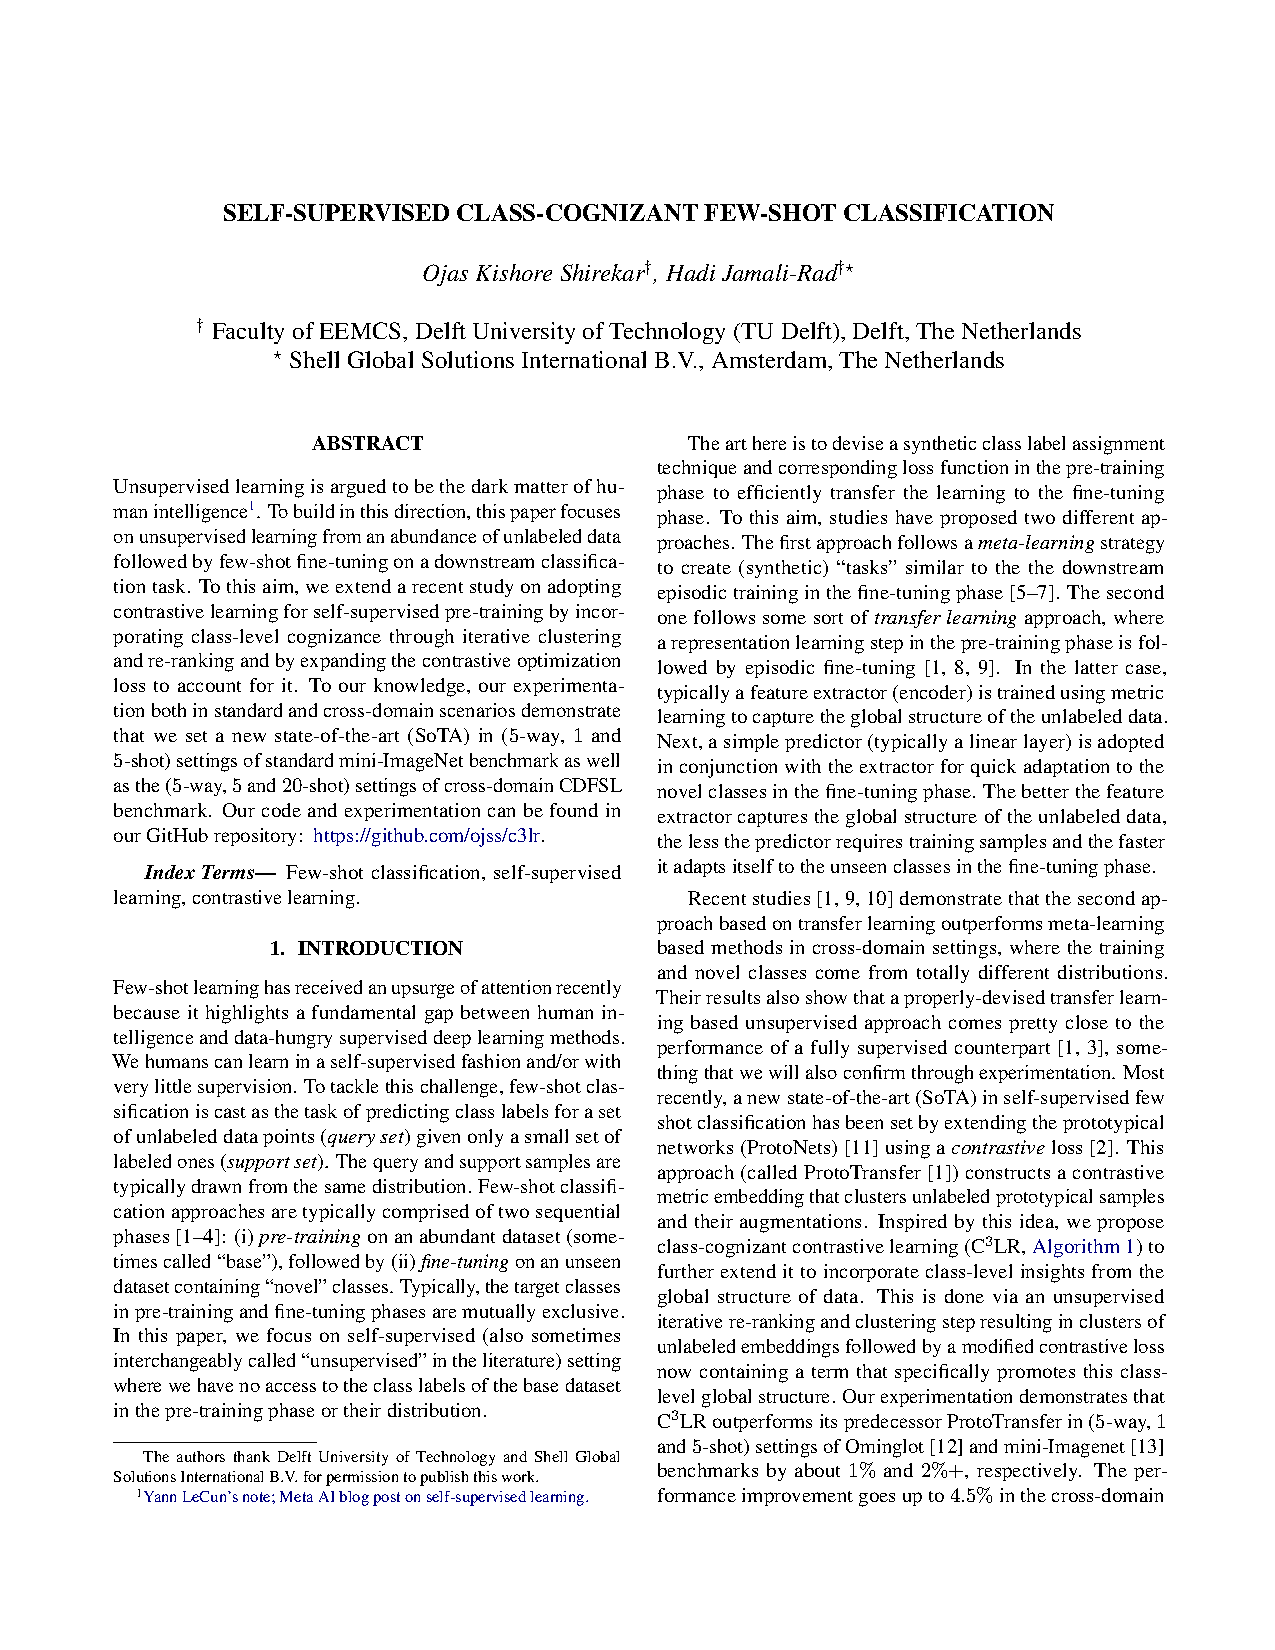
\includepdf[pages=-, pagecommand={}]{chapters/articles/c3lr/ICIP_C3LR_final.pdf}

% \chapter{Template Info}

This document is intended to be both an example of the TU Delft \LaTeX{} template for reports and theses, as well as a short introduction to its use. It is not intended to be a general introduction to \LaTeX{} itself,\footnote{We recommend \url{http://en.wikibooks.org/wiki/LaTeX} as a reference and a starting point for new users.} and we will assume the reader to be familiar with the basics of creating and compiling documents.

Instructions on how to use this template under Windows and Linux, and which \LaTeX{} packages are required, can be found in \texttt{README.txt}.

\section{Document Structure}

Since a report, and especially a thesis, might be a substantial document, it is convenient to break it up into smaller pieces. In this template we therefore give every chapter its own file. The chapters (and appendices) are gathered together in \texttt{report.tex}, which is the master file describing the overall structure of the document. \texttt{report.tex} starts with the line
\begin{verbatim}
    \documentclass{tudelft-report}
\end{verbatim}
which loads the TU Delft report template. The template is based on the \LaTeX{} \texttt{book} document class and stored in \texttt{tudelft-report.cls}. The document class accepts several comma-separated options. The default language is English, but this can be changed to Dutch (\emph{e.g.}, for bachelor theses) by specifying the \texttt{dutch} option:
\begin{verbatim}
    \documentclass[dutch]{tudelft-report}
\end{verbatim}
Furthermore, hyperlinks are shown in blue, which is convenient when reader the report on a computer, but can be expensive when printing. They can be turned black with the \texttt{print} option. This will also turn the headers black instead of cyan.

If the document becomes large, it is easy to miss warnings about the layout in the \LaTeX{} output. In order to locate problem areas, add the \texttt{draft} option to the \verb|\documentclass| line. This will display a vertical bar in the margins next to the paragraphs that require attention. Finally, the \texttt{nativefonts} option can be used to override the automatic font selection (see below).

This template has the option to automatically generate a cover page with the \verb|\makecover| command. See the next section for a detailed description.

The contents of the report are included between the \verb|\begin{document}| and \verb|\end{document}| commands, and split into three parts by
\begin{enumerate}
\item\verb|\frontmatter|, which uses Roman numerals for the page numbers and is used for the title page and the table of contents;
\item\verb|\mainmatter|, which uses Arabic numerals for the page numbers and is the style for the chapters;
\item\verb|\appendix|, which uses letters for the chapter numbers, starting with `A'.
\end{enumerate}
The title page is defined in a separate file, \emph{e.g.}, \texttt{title.tex}, and included verbatim with \verb|\begin{titlepage}


\begin{center}

%% Insert the TU Delft logo at the bottom of the page.

%% Print the title in cyan.
{\makeatletter
\largetitlestyle\fontsize{64}{94}\selectfont\@title
%\largetitlestyle\color{tudelft-cyan}\Huge\@title
\makeatother}

%% Print the optional subtitle in black.
{\makeatletter
\ifx\@subtitle\undefined\else
    \bigskip
   {\tudsffamily\fontsize{22}{32}\selectfont\@subtitle}    
    %\titlefont\titleshape\LARGE\@subtitle
\fi
\makeatother}

\bigskip
\bigskip

by
%door

\bigskip
\bigskip

%% Print the name of the author.
{\makeatletter
%\largetitlefont\Large\bfseries\@author
\largetitlestyle\fontsize{26}{26}\selectfont\@author
\makeatother}

\bigskip
\bigskip

to obtain the degree of Master of Science
%ter verkrijging van de graad van Master of Science

at the Delft University of Technology,
%aan de Technische Universiteit Delft,

to be defended publicly on Wednesday August 31, 2022 at 14:30.
%in het openbaar de verdedigen op dinsdag 1 januari om 10:00 uur.

\vfill

\begin{tabular}{lll}
    Student number: & 5225493 \\
    Project duration: & \multicolumn{2}{l}{July 1, 2021 -- July 31, 2022} \\
    Thesis committee: & Dr.\ H.\ Jamali-Rad, & TU Delft and Shell, Daily supervisor \\
        & Dr.\ ir.\ J.\ van Gemert, & TU Delft, Advisor \\
        & Dr.\ E.\ Isufi, & TU Delft, External committee member
\end{tabular}
%% Only include the following lines if confidentiality is applicable.

\bigskip
\bigskip
% \emph{This thesis is confidential and cannot be made public until December 31, 2013.}
%\emph{Op dit verslag is geheimhouding van toepassing tot en met 31 december 2013.}

\bigskip
\bigskip
An electronic version of this thesis is available at \url{http://repository.tudelft.nl/}.
%\\[1cm]

%\centering{
\includegraphics{cover/logo_black}}


\end{center}

\begin{tikzpicture}[remember picture, overlay]
    \node at (current page.south)[anchor=south,inner sep=0pt]{
        
\includegraphics{cover/logo_black}
    };
\end{tikzpicture}

\end{titlepage}

|.\footnote{Note that it is not necessary to specify the file extension.} Additionally, it is possible to include a preface, containing, for example, the acknowledgements. An example can be found in \texttt{preface.tex}. The table of contents is generated automatically with the \verb|\tableofcontents| command. Chapters are included after \verb|\mainmatter| and appendices after \verb|\appendix|. For example, \verb|input{chapter-1}| includes \texttt{chapter-1.tex}, which contains this introduction.

\subsection{Bibliography}

Lists of references are handled by \texttt{biblatex}.
The present document has the following preamble
\begin{verbatim}
\usepackage[style=apa]{biblatex}
\addbibresource{report.bib}
\end{verbatim}
The first line tells us that the references will be formatted according 
to the APA-standards.
On \texttt{Overleaf} this should adhere to the 7th version of these 
standards.
On your own computer the version of biblatex may be older and 
use the 6th~version.

The second line points to a file that contains the references in a database
like format.
Use one such line for every database that you want to use.

The general way this works is as follows Using the present document as 
an example):
\begin{verbatim}
xelatex report
biber report
xelatex report
\end{verbatim}
The first line typesets the document and gathers information for the lists
of references; the second line will generate lists of references for all 
chapters, these will be read in during execution of the third and fourth lines.
Depending on the editor that you use much of this can be done by clicking
on a suitable icon or by hitting suitably defined hot keys.

The \texttt{biblatex} package has many options and can be tailored to almost
every need; you can explore its documentation at
\texttt{https://www.ctan.org/pkg/biblatex}

To get numbered references just use
\begin{verbatim}
\usepackage{biblatex}
\addbibresource{report.bib}
\end{verbatim}

To give some examples we cite an article: \cite{Einstein1906},
a book: \cite{MR1039321}, another article: \cite{MR3860876},
and a book with more than one editor: \cite{MR3204729}.




\section{Cover and Title Page}

This template will automatically generate a cover page if you issue the \verb|\makecover| command. There are two formats for the cover page: one with a page-filling (`bleeding')
illustration, with the title(s) and author(s) in large ultrathin typeface, and the other where the illustration fills the lower half of the A4, whereas title(s), author(s) and additional
text are set in the standard sans-serif font on a plain background with a color chosen by the user. The last option is selected by the optional key \texttt{split}: \verb|\makecover[split]| yields
a page with the illustration on the lower half. All illustrations are bleeding, in accordance with the TU Delft style.

Before generating the cover, you need to provide the information to put on it. This can be done with the following commands:
\begin{itemize}
\item\verb|\title[Optional Color]{Title}| \\
    This command is used to provide the title of the document. The title
    title is also printed on the spine. If you use a title page (see below), this information will be used there as well.
    As the title, subtitle and author name are printed directly over the cover photo, it will often be necessary to adjust the print color in order to have
    sufficient contrast between the text and the background. The optional color argument is used for this.
\item\verb|\title[Optional Color]{Subtitle}| \\
    This command is used to provide a subtitle for the document. If you use a title page (see below), this information will be used there as well.
    It possible to adjust the print color in order to have
    sufficient contrast between the text and the background -- the optional color argument is used for this.
\item\verb|\author{J.\ Random Author}| \\
    This command specifies the author. The default color is \texttt{tudelft-white}, but this may be adjusted in the same way as the titles.
\item\verb|\affiliation{Technische Universiteit Delft}| \\
    The affiliation is the text printed vertically on the front cover. It can be the affiliation, such as the university or department name, or be used for the document type (\emph{e.g.}, Master's thesis). The default color is again \texttt{tudelft-white}, adjustable through the \texttt{color} option.
\item\verb|\coverimage{cover.jpg}| \\
    With this command you can specify the filename of the cover image. The image is stretched to fill the full width of the front cover (including the spine if a back cover is present).
\item\verb|\covertext{Cover Text}| \\
    If a back cover is present, the cover text is printed on the back. Internally, this text box is created using the \LaTeX{} \texttt{minipage} environment, so it supports line breaks.
\item\verb|\titleoffsetx{OffsetX},\titleoffsety{OffsetY}|
    If the cover page contains a page-filling picture (i.e., \texttt{split} is not specified with the \texttt{makecover} command, the best position of the title depends a lot on the picture chosen for it. The lower left corner of the minipage containing title, subtitle and author is 
    specified by these two commands. The offsets are measured from the top left corner of the page. 
\item\verb|\afiloffsetx{AfilX\}, \afiloffsety{AfilY}|
    specifies the lower left corner of the text containing the affiliation, measured from the top left corner of the page. 
\end{itemize}

In addition to \texttt{[split]}, the \verb|\makecover| command accepts several additional options for customizing the layout of the cover. 
The most important of these is \texttt{back}. Supplying this option will generate a back cover as well as a front, including the spine. Since this requires a page size slightly larger than twice A4 (to make room for the spine), and \LaTeX{} does not support different page sizes within the same document, it is wise to create a separate file for the cover. \texttt{cover.tex} contains an example. The recommended page size for the full cover can be set with
\begin{verbatim}
    \geometry{papersize={1226bp,851bp}}
\end{verbatim}
after the document class and before \verb|\begin{document}|.

The other options \verb|\makecover| accepts are
\begin{itemize}
\item\texttt{nospine} \\
    If a back cover is generated, the title will also be printed in a black box on the spine. However, for smaller documents the spine might not be wide enough. Specifying this option disables printing the title on the spine.
\item\texttt{frontbottom} \\
    By default the black box on the front is situated above the blue box. Specifying this option will place the black box below the blue one.
\item\texttt{spinewidth} \\
    If a back cover is present, this option can be used to set the width of the spine. The default is \texttt{spinewidth=1cm}.
\item\texttt{frontboxwidth}, \texttt{frontboxheight}, \texttt{backboxwidth}, \texttt{backboxheight} \\
    As their names suggest, these options are used to set the width and height of the front (black) and back (blue) boxes. The default widths and heights are \texttt{4.375in} and \texttt{2.1875in}, respectively.
\item\texttt{x}, \texttt{y} \\
    The blue and black boxes touch each other in a corner. The location of this corner can be set with these options. It is defined with respect to the top left corner of the front cover. The default values are \texttt{x=0.8125in} and \texttt{y=3in}.
\item\texttt{margin} \\
    This option sets the margin between the borders of the boxes and their text. The default value is \texttt{12pt}.
\end{itemize}

For a thesis it is desirable to have a title page within the document, containing information like the thesis committee members. To give you greater flexibility over the layout of this page, it is not generated by a command like \verb|\makecover|, but instead described in the file \texttt{title.tex}. Modify this file according to your needs. The example text is in English, but Dutch translations are provided in the comments. Note that for a thesis, the title page is subject to requirements which differ by faculty. Make sure to check these requirements before printing.

\section{Chapters}

Each chapter has its own file. For example, the \LaTeX{} source of this chapter can be found in \texttt{chapter-1.tex}. A chapter starts with the command
\begin{verbatim}
    \chapter{Chapter title}
\end{verbatim}
This starts a new page, prints the chapter number and title and adds a link in the table of contents. If the title is very long, it may be desirable to use a shorter version in the page headers and the table of contents. This can be achieved by specifying the short title in brackets:
\begin{verbatim}
    \chapter[Short title]{Very long title with many words 
        which could not possibly fit on one line}
\end{verbatim}
Unnumbered chapters, such as the preface, can be created with \verb|\chapter*{Chapter title}|. Such a chapter will not show up in the table of contents or in the page header. To create a table of contents entry anyway, add
\begin{verbatim}
    \addcontentsline{toc}{chapter}{Chapter title}
\end{verbatim}
after the \verb|\chapter| command. To print the chapter title in the page header, add
\begin{verbatim}
    \setheader{Chapter title}
\end{verbatim}

Chapters are subdivided into sections, subsections, subsubsections, and, optionally, paragraphs and subparagraphs. All can have a title, but only sections and subsections are numbered. As with chapters, the numbering can be turned off by using \verb|\section*{\ldots}| instead of \verb|\section{\ldots}|, and similarly for the subsection.
\section{\textbackslash section\{\ldots\}}
\subsection{\textbackslash subsection\{\ldots\}}
\subsubsection{\textbackslash subsubsection\{\ldots\}}
\paragraph{\textbackslash paragraph\{\ldots\}}
Lorem ipsum dolor sit amet, consectetur adipisicing elit, sed do eiusmod tempor incididunt ut labore et dolore magna aliqua. Ut enim ad minim veniam, quis nostrud exercitation ullamco laboris nisi ut aliquip ex ea commodo consequat. Duis aute irure dolor in reprehenderit in voluptate velit esse cillum dolore eu fugiat nulla pariatur. Excepteur sint occaecat cupidatat non proident, sunt in culpa qui officia deserunt mollit anim id est laborum.

\section{Fonts and Colors}

The fonts used by this template depend on which version of \LaTeX{} you use. Regular \LaTeX, \emph{i.e.}, if you compile your document with with \texttt{latex}, \texttt{pslatex} or \texttt{pdflatex}, will use Utopia for text, Fourier for math and Latin Modern for sans-serif and monospaced text. 
However, if you want to adhere to the TU Delft house style, you will need to use \XeLaTeX, as it supports TrueType and OpenType fonts. Compiling with \texttt{xelatex} will use Arial for most titles and text, Courier New for monospace and Cambria for math. If you want to haf a sans-serif font for the
main text, while using \texttt{latex}, \texttt{pslatex} or \texttt{pdflatex}, you can use the option \texttt{noroman} in the report style: 
\begin{verbatim}
   \documentclass[...,noroman]{tudelft-report}
\end{verbatim}
For document and part titles,  TU Delft Ultra Light is used. For quotes, columns and text in boxes, you use Georgia. If you want to use \XeLaTeX, but do not want to use the TU Delft house style fonts, you can add the \texttt{nativefonts} option to the document class. This will still use  TU Delft Utra Light and Arial on the cover, but not for the body of the document. If you need to use these fonts for certain sections in the main text, they are available via \verb|\tudrmfamily| (Georgia) and \verb|\tudtitlefamily| (TU Delft Utra Light).

\begin{quote}
  You have to learn the rules of the game. And then you have to play better than anyone else.\\
  \emph{Albert Einstein}
\end{quote}

The corporate colors of the TU Delft are cyan, black and white, available via 
{\color{tudelft-cyan}\verb|\color{tudelft-cyan}|}, 
{\color{tudelft-black}\verb|\color{tudelft-black}|} 
(which differs slightly from the default 
{\color{black}\verb|\color{black}|}) 
and \verb|\color{tudelft-white}|, respectively. 
Apart from these three, the house style defines the basic colors \texttt{\color{tudelft-sea-green}tudelft-sea-green}, \texttt{\color{tudelft-green}tudelft-green}, \texttt{\color{tudelft-dark-blue}tudelft-dark-blue}, \texttt{\color{tudelft-purple}tudelft-purple}, \texttt{\color{tudelft-turquoise}tudelft-turquoise} and \texttt{\color{tudelft-sky-blue}tudelft-sky-blue}, as well as the accent colors \texttt{\color{tudelft-lavendel}tudelft-lavendel}, \texttt{\color{tudelft-orange}tudelft-orange}, \texttt{\color{tudelft-warm-purple}tudelft-warm-purple}, \texttt{\color{tudelft-fuchsia}tudelft-fuchsia}, \texttt{\color{tudelft-bright-green}tudelft-bright-green} and \texttt{\color{tudelft-yellow}tudelft-yellow}.



% \chapter{Deep Learning} \label{chap:basics-of-dl}

Deep learning is an area of machine learning that uses Artificial Neural Networks \parencite{mcculloch1943logical} and has been applied to a wide variety of tasks such as image classification, object recognition, activity recognition, 3D depth estimation, and various natural language processing (NLP) tasks. In stark contrast to the classical machine learning approach of designing manual feature extraction methods, deep learning focuses on creating algorithms that can automatically learn to extract relevant features.

\section{Deep Feedforward Networks} \label{sec:feed-forward-nets}

Deep feedforward networks, also called feedforward networks, or \textbf{multilayer perceptrons} (MLPs), are essential deep learning models. The goal of a feedforward network is to approximate some ideal function \(f^\star\). 
For example, a classifier \(y = f^\star(\symbfit{x})\) is a mapping between input $\symbfit{x}$ to a category $y$. A feedforward network has the ability to learn this mapping \(\symbfit{y} = f(\symbfit{x} \mathsemicolon \symbfit{\theta})\) where $\symbfit{\theta}$ is a set of learnt parameters that results in the best approximation of function $f(\symbfit{x} \mathsemicolon \symbfit{\theta}) \approx f^\star$. In other words, neural networks are function approximators.

These models are called \textbf{feedforward} because the information flows through the function that evaluates $\symbfit{x}$ and produces $\symbfit{y}$. The process of passing the input $\symbfit{x}$ through the function and through intermediate computations is known as \textbf{forward pass}.
We then use a \textbf{loss function} to measure the difference between $f^\star$ and $f$ - that is, the difference between the ideal mapping $f^\star$ and the estimated mapping $f$. 
The parameters of the network, $\symbfit{\theta}$, are updated in a \textbf{backward pass} based on some optimisation criteria, given the guidance of the loss function. 

% \includesvg{./assets/mlp.svg}
% \begin{figure}
%     \centering
%     % \captionsetup{justification=RaggedRight}
%     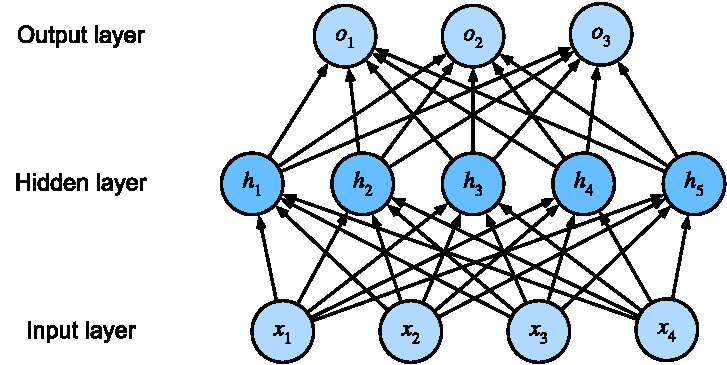
\includegraphics[scale=0.9]{chapters/assets/mlp.pdf}
%     \caption{An MLP with hidden layer consisting of $5$ hidden units. Image courtesy of \textcite{zhang2021dive}.}
%     \label{fig:mlp}
% \end{figure}
\def\layersep{2.5cm}
\begin{figure}
    \centering
    \captionsetup{justification=centering}
    \begin{tikzpicture}[shorten >=1pt,->,draw=black!50, node distance=\layersep]
    \tikzstyle{every pin edge}=[<-,shorten <=1pt]
    \tikzstyle{neuron}=[circle,fill=black!25,minimum size=17pt,inner sep=0pt]
    \tikzstyle{input neuron}=[neuron, fill=tudelft-green!50];
    \tikzstyle{output neuron}=[neuron, fill=tudelft-fuchsia!40];
    \tikzstyle{hidden neuron}=[neuron, fill=tudelft-cyan!50];
    \tikzstyle{annot} = [text width=4em, text centered]

    % Draw the input layer nodes
    \foreach \name / \y in {1,...,4}
    % This is the same as writing \foreach \name / \y in {1/1,2/2,3/3,4/4}
        \node[input neuron, pin=left:Input \#\y] (I-\name) at (0,-\y) {\(\symbfit{x}_{\y}\)};

    % Draw the hidden layer nodes
    \foreach \name / \y in {1,...,5}
        \path[yshift=0.5cm]
            node[hidden neuron] (H-\name) at (\layersep,-\y cm) {\(\symbfit{h}_{\y}\)};

    % Draw the output layer node
    \node[output neuron,pin={[pin edge={->}]right:Output}, right of=H-3] (O-0) {\(\symbfit{o}_{1}\)};
    \node[output neuron,pin={[pin edge={->}]right:Output}, right of=H-2] (O-1) {\(\symbfit{o}_{2}\)};
    \node[output neuron,pin={[pin edge={->}]right:Output}, right of=H-4] (O-2) {\(\symbfit{o}_{3}\)};

    % Connect every node in the input layer with every node in the
    % hidden layer.
    \foreach \source in {1,...,4}
        \foreach \dest in {1,...,5}
            \path (I-\source) edge (H-\dest);

    % Connect every node in the hidden layer with the output layer
    \foreach \source in {1,...,5}
        \foreach \dest in {0,...,2}
            \path (H-\source) edge (O-\dest);

    % Annotate the layers
    \node[annot,above of=H-1, node distance=1cm] (hl) {Hidden layer};
    \node[annot,left of=hl] {Input layer};
    \node[annot,right of=hl] {Output layer};
\end{tikzpicture}
    \caption{An MLP with a hidden layer consisting of $5$ hidden units.}
    \label{fig:mlp}
\end{figure}

Feedforward neural networks are called \textit{networks} because they are typically composed of many different functions. The model is associated with a directed acyclic graph that describes how the functions are composed together.
For example, we can have three functions \(f^{(1)}, f^{(2)}\) and $f^{(3)}$ connected in a chain, to form \(f = f^{(1)} \circ f^{(2)} \circ f^{(3)}\). 
Chain structures such as these are quite commonly used structures of neural networks. Here, $f^{(1)}$ is the \textbf{first layer}, $f^{(2)}$ is the \textbf{second layer} and so on. 
The final layer is called \textbf{output layer}, in this small example, $f^{(3)}$ is the output layer. The training data and training strategy determine what the output layer must produce for each given input $\symbfit{x}$.
Intermediate layers such as $f^{(2)}$ that do not directly produce the output $\symbfit{y}$ are called \textbf{hidden layers}.

Each hidden layer of the network is typically vector valued. The dimensionality of these hidden layers determines \textbf{width} of the model. Each element in the vector plays a role analogous to a neuron. Instead of thinking of a layer as a vector-to-vector function, we can also think of the layer as consisting of many \textbf{units} that act in parallel \parencite{Pinker1988}, each representing a vector-to-scalar function. 
\Cref{fig:mlp} shows a small MLP with a single hidden layer. Each of the nodes in \cref{fig:mlp} represents a value in a vector; this implies that the input $\symbfit{x}$ has a dimensionality of $4$, the hidden layer (intermediate values) has a dimensionality of $5$ and the output has a dimensionality of $3$.

Now, we must choose the form of our model, $f(\symbfit{x} \mathsemicolon \symbfit{\theta})$. Let us choose a linear model parameterised by $\symbfit{\theta}$ consisting of $\symbfit{w}$ and $b$, where $\symbfit{w}$ provides the \textbf{weights} and $b$ provides the \textbf{biases} (or intercepts):
\begin{equation}
    \label{eqn:linear-model}
    f(\symbfit{x}; \symbfit{\theta}) = f(\symbfit{x} ; \symbfit{w}, b)=\symbfit{x}^{\top} \symbfit{w} + b.
\end{equation}

For the model in \cref{fig:mlp} whose hidden layer has $\symbfit{h}$ units, which are calculated by a function \(f^{(1)}(\symbfit{x}; \symbfit{W}, \symbfit{c})\) that is linear similar to the form of \cref{eqn:linear-model}. 
The values of these hidden units are then used as input to the second layer, which is also the output layer of the network. The output layer is also a linear function applied to $\symbfit{h}$ rather than to $\symbfit{x}$.
The network now has two functions chained together \(\symbfit{h} = f^{(1)}(\symbfit{x}; \symbfit{W}, \symbfit{c})\) and \(y = f(\symbfit{h} ; \symbfit{w}, b)\), with the complete model being $f(\symbfit{x} ; \symbfit{W}, \symbfit{c}, \symbfit{w}, b)=f^{(2)}\left(f^{(1)}(\symbfit{x})\right)$. It should be noted that a model parameterised by $\symbfit{\theta}$ implies that $\symbfit{\theta}$ is a collection of all the weights and biases present in the network.

Unfortunately, the complete model $f$ is a linear function of its input, since we have chosen both $f^{(1)}$ and $f^{(2)}$ to be linear. 
However, not all data spaces are linear. More often than not, they are non-linear in nature; accordingly, we must introduce a non-linear function to describe the data and its features.
Most neural networks do so using an \textbf{affine transformation} controlled by the learned parameters (such as $\symbfit{\theta}$), followed by a fixed nonlinear function called an \textbf{activation function}.

\section{Activation Functions} \label{sec:activation-functions}

Activation functions decide whether or not a neuron (node in \cref{fig:mlp}) should be activated. More specifically, they are differentiable operators to transform inputs to outputs and add some form of non-linearity in the transformation. Formally, our hidden-layer output is now defined as:
% \begin{equation}
%     f(\symbfit{x}; \symbfit{\theta}) = f(\symbfit{x}; \symbfit{w}, b) = g(\symbfit{x}^\top\symbfit{w} + b)
% \end{equation}
\begin{equation}
\begin{split}
    \symbfit{h} &= g \circ f^{(1)} \left(\symbfit{x}\right)\\
                &=g\left(\symbfit{W}^{\top} \symbfit{x}+\symbfit{c}\right)
\end{split}
\end{equation}
where $\symbfit{W}$ is the linear transformation, $\symbfit{c}$ the biases and $g(\cdot)$ is an \textbf{activation function} whose job is to introduce some non-linearity. Previously, we had used a vector of weights and a scalar bias parameter in \cref{eqn:linear-model} to describe an affine transformation from a vector input to a scalar output. However, now we are describing an affine transformation from a vector $\symbfit{x}$ to a vector $\symbfit{h}$, so an entire vector of biases is needed.

One of the most widely used activation functions is \textbf{ReLU} (Rectified Linear Unit) \parencite{Fukushima1975}. This function simply returns the maximum between the given input value and zero, as given in \cref{eqn:relu}. As such, this simple function has a minimal computation cost and can be performed quite quickly.
\begin{equation}\label{eqn:relu}
    \begin{split}
        g \circ f(\symbfit{x}) & = \operatorname{max}\left(0, f^{(1)}(\symbfit{x})\right)\\
                               & = \operatorname{max}\left(0, \symbfit{W}^\top\symbfit{x} + \symbfit{c}\right)
    \end{split}
\end{equation}

Another important and common function is the \textbf{Sigmoid} \cref{eqn:sigmoid} function. This function maps the input value to a real number between $(0, 1)$.
In earlier forms of nerural networks \parencite{mcculloch1943logical}, scientists where interested in neurons that either fire or do not, and so used thresholding units. A thresholding activation takes value $0$ when its input is below a certain threshold and takes value $1$ if its input is higher than the threshold. 
Sigmoids, on the other hand, are smooth and differentiable approximations of thresholding units; this is favourable to the gradient-based learning adopted in today's time.
Sigmoids are used largely in output units when we want to interpret the output as probabilities for binary classification problems.
\begin{equation}\label{eqn:sigmoid}
    \begin{split}
        \operatorname{sigmoid}(\symbfit{x}) = \sigma(\symbfit{x}) & = \frac{1}{1 + \exp(-\symbfit{x})}.
        % \operatorname{sigmoid}(\symbfit{h}) & = \frac{1}{1 + \exp(-(\symbfit{W}^\top\symbfit{x}+\symbfit{c}))}.
    \end{split}
\end{equation}

Like the sigmoid function, the \textbf{tanh} (hyperbolic tan) function also squashes its inputs, mapping them between $-1$ and $1$:
\begin{equation}
\begin{split}
    \operatorname{tanh}(\symbfit{x}) & = \frac{1 - \exp(-2\symbfit{x})}{1 + \exp(-2\symbfit{x})}.
    % \operatorname{tanh}(\symbfit{h}) & = \frac{1 - \exp(-2(\symbfit{W}^\top\symbfit{x}+\symbfit{c}))}{1 + \exp(-2(\symbfit{W}^\top\symbfit{x}+\symbfit{c}))}.
\end{split}
\end{equation}

\begin{figure}[t]
     \centering
     \captionsetup{justification=centering}
     \begin{subfigure}[b]{0.3\textwidth}
         \centering
         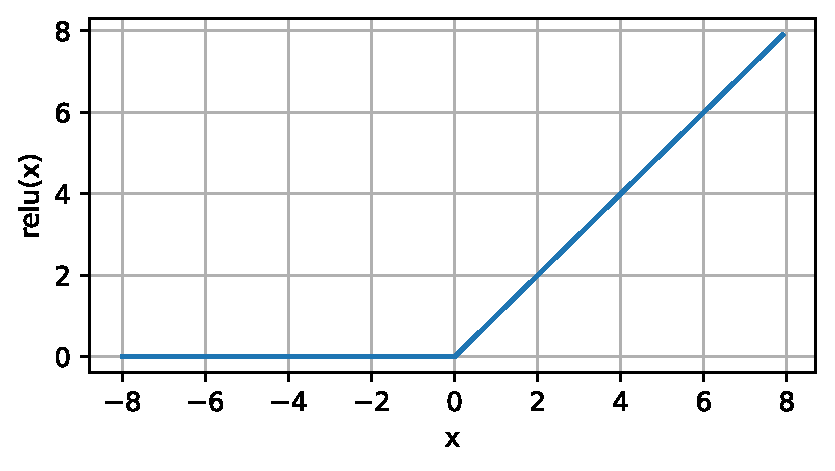
\includegraphics[width=\textwidth]{chapters/assets/relu.pdf}
         \caption{ReLU}
         \label{fig:relu}
     \end{subfigure}
     \hfill
     \begin{subfigure}[b]{0.3\textwidth}
         \centering
         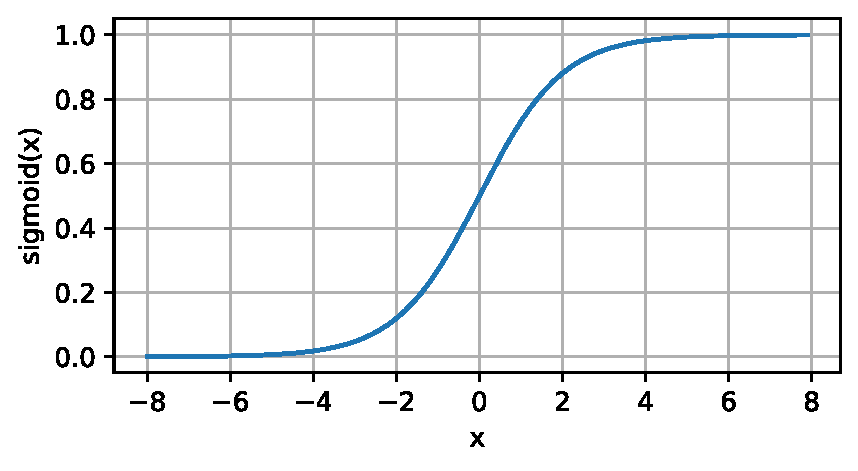
\includegraphics[width=\textwidth]{chapters/assets/sigmoid.pdf}
         \caption{Sigmoid}
         \label{fig:sigmoid}
     \end{subfigure}
     \hfill
     \begin{subfigure}[b]{0.3\textwidth}
         \centering
         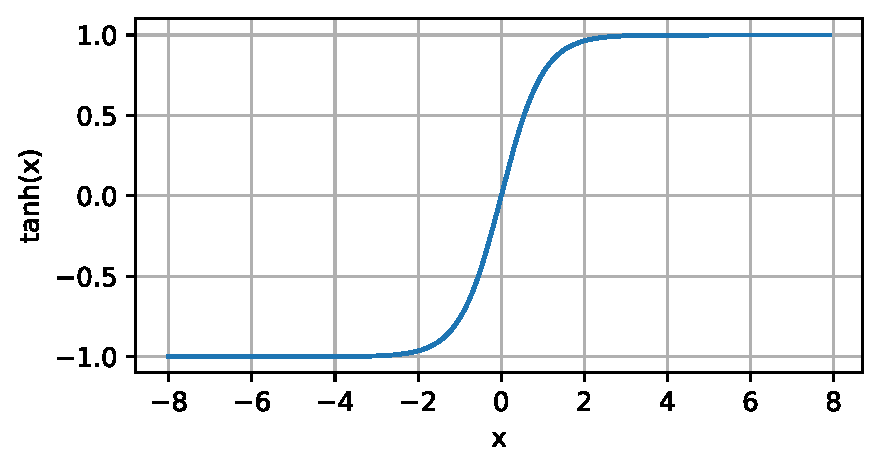
\includegraphics[width=\textwidth]{chapters/assets/tanh.pdf}
         \caption{Tanh}
         \label{fig:tanh}
     \end{subfigure}
        \caption{Three common activation functions.}
        \label{fig:three-activation-funcs}
\end{figure}

\section{Loss Function}\label{sec:loss-fn}
During training, for each training sample in the training set $\{\symbfit{x}_i, y_i\}_{i=1}^N$ where $\symbfit{x}_i$ is an input vector and $y_i$ is the corresponding label, we present the input $\symbfit{x}$ to the neural network and compare the predicted output of the network $\hat{y}_i$ with the corresponding label $y_i$.
We need to define a \textbf{loss function} to objectively measure how much the predicted output of the network $\hat{y}_i$ is different from the expected output $y_i$. For regression problems, the quadratic loss function called the mean squared error (MSE) is calculated as follows:
\begin{equation}
    \mathcal{L}({\hat{y}}, {y}) = \frac{1}{2} \| {y} - {\hat{y}} \| ^ 2
\end{equation}

The loss function is calculated for each training example in the training set. The average of the calculated loss functions for all training examples in the training set is called the \textbf{cost function}. For MSE it is the average of the calculated loss functions for all training examples in the training set:
\begin{equation}
    J(\symbfit{\theta}) = \frac{1}{2N} \sum_{i=1}^{N} \| {y}_i - {\hat{y}_i} \| ^ 2
\end{equation}
where $N$ is the total number of training samples. In the following \Cref{sec:softmax} we shall see another loss function that is important for multiclass classification.

\section{Softmax} \label{sec:softmax}
For convenience in the following section, we shall call the output of network $f(\symbfit{x}; \symbfit{\theta})$ as $\symbfit{o}$. Assume that we have a loss function such as mean squared error loss (MSE). When working with \textbf{multiclass classification} problems, where \(\symbfit{y} \in \left\{1,\ldots, K \right\}\); we expect the output of the model to be a vector of class probabilities where each value tells us the probability that a sample belongs to a particular class.
Note that we generally employ the ``one-hot'' encoding mechanism where $\symbfit{y} = (0, ... , 0, 1, 0, ... , 0)$.
We can try to directly minimise the difference between $\symbfit{o}$ and $\symbfit{y}$. Although treating classification as a regression problem may work well, it still lacks in two main ways:
\begin{itemize}
    \item There is no guarantee that $\symbfit{o}$ will sum up to $1$ as we have come to expect from probabilities
    \item There is no guarantee that $\symbfit{o}$ takes strictly non-negative values regardless of the sum of $\symbfit{o}$
\end{itemize}

Both of these issues make the problem difficult to solve in addition to making the solution highly sensitive to outliers. If we were to presume a positive linear dependency between the horsepower of a car and the probability that someone will buy it, the probability might exceed $1$ when it comes to buying a Bugatti Chiron\footnote{\url{https://www.bugatti.com/models/chiron-models/}}! Of course, this breaks the mathematical and logical rules of probability theory; therefore, we need a technique to map the values of $\symbfit{o}$ between $(0, 1)$.
% TODO: should we talk about data generating distribution here?

One way to accomplish these goals (ensuring that the output sums up to $1$ and its values are non-negative), is to use an exponential function $P(y = i) \propto \exp o_i$. The $\exp$ function does ensure that the output will always be non-negative. We can further \textbf{normalise} these values so that they add up to $1$ by dividing each by the sum of the whole. This gives us the \textbf{softmax} function:
\begin{equation}
    \hat{\symbfit{y}} = \operatorname{softmax}(\symbfit{o}) \quad \text{where}\quad \hat{y}_i = \frac{\exp(o_i)}{\sum_{j=1}^{K} \exp(o_j)}.
    \label{eqn:std-softmax}
\end{equation}

Note that the highest value in $\symbfit{o}$ corresponds to the most likely class according to $\symbfit{\hat{y}}$. Softmax also preserves the ordering of its arguments as shown in the example:
\begin{equation}
    \nonumber
    \operatorname{softmax} \left(\begin{bmatrix}
    8\\
    5\\
    0
    \end{bmatrix}\right)
    = 
    \begin{bmatrix}
    0.9523\\
    0.0474\\
    0
    \end{bmatrix}.
\end{equation}

\subsection{Softmax and Cross-Entropy Loss}\label{ssec:ce-loss}

The softmax function gives us a vector $\symbfit{\hat{y}}$, which we can interpret as (estimated) conditional probabilities of each class, given any input $\symbfit{x}$, like $P(y=\text{class} | \symbfit{x})$. 
The cross-entropy loss measures the difference between two probability distributions; in this case, it measures the difference between $\symbfit{\hat{y}}$ and $\symbfit{y}$. The cross-entropy loss is given as:
\begin{equation}\label{eqn:ce-loss}
    \mathcal{L}(\symbfit{y}, \hat{\symbfit{y}}) = - \sum_{j=1}^K \symbfit{y}_j \log \hat{\symbfit{y}}_j.
\end{equation}

Note that the loss defined in \cref{eqn:ce-loss}, has a lower bound of $0$ when $\hat{\symbfit{y}}$ is a probability vector, that is, no single entry is greater than $1$, and hence its negative logarithm cannot be lower than $0$. For multiclass classification problems, the cost function is calculated as follows:
\begin{equation}
    J(\symbfit{\theta}) = - \frac{1}{N} \sum_{j=1}^{N} \sum_{i=1}^{K} \symbfit{y_{i}^{(j)}}\log(\symbfit{\hat{y}_{i}^{(j)}})
\end{equation}
where $\symbfit{y_{i}^{(j)}}$ and $\symbfit{\hat{y}_{i}^{(j)}}$ are the true and predicted output for the $j\textsuperscript{th}$ input sample $\symbfit{x}_j$. To better understand the origins of the cross-entropy loss, please refer to \textcite{zhang2021dive}.

\subsection{Softmax vs Sigmoid}\label{ssec:softmax-vs-sigmoid}
The softmax and sigmoid functions are similar, as they help squeeze the network output within a certain range. The softmax function operates on a vector input, while the sigmoid takes a scalar value as input. In fact, the sigmoid function is a special case of the softmax function for a classifier with only two input classes (binary classification problem). We can show this if we set the input vector to $\symbfit{z} = [x, 0]$ and calculate the first output element with the usual softmax formula:
\begin{align*}
    \operatorname{softmax}(\symbfit{z})_{1}&=\frac{\exp{(z_{1})}}{\exp{(z_{1})}+\exp(z_{2})} \\
    &= \frac{\exp(x)}{\exp(x)+\exp(0)} \\
    &= \frac{\exp(x)}{\exp(x)+1} && \text{divide numerator and denominator by} \exp{(x)}\\
    &= \frac{1}{1 + \exp(-x)}
\end{align*}


\section{Universal Approximation Theory}\label{sec:uat}

MLPs are of extreme importance in deep learning, as they form the basis for many applications and advanced neural architectures. To do this, MLPs and neural networks, in general, must be able to approximate a wide range of functions, given enough input data to learn from. Neural networks started as a way to mimic the neural structure of the brain \parencite{mcculloch1943logical}, and as we know our brain is capable of complex statistical analysis, among other things. As such, a worthwhile question to ask here is \textit{just how powerful can a deep neural network be?}
Fortunately for us, this question has been answered several times in the context of MLPs and radial basis functions (RBF) \parencite{Cybenko1989, Micchelli1986, Hornik1991}. These works suggest that even with a single hidden layer, given enough nodes and the right set of parameters $\symbfit{\theta}$, we can potentially model any function. 
In simple terms, having enough nodes and stacking enough affine transformations followed by non-linear transforms repetitively, a neural network should be able to model a highly rich class of functions.
Although neural networks are capable of expressing arbitrary continuous functions, it may not be easy to learn the function and its parameters.

\section{Optimisation and Backpropagation}\label{sec:optimisation}

Until now, we have only discussed the forward pass of a neural network, where the network processes the input $\symbfit{x}$. However, to effectively approximate $f^\star$, a neural network must learn an ideal set of values for the parameters, $\symbfit{\theta}$. To do so, we must \textbf{optimise} the weights so that they are suitable for the task and the data at hand. However, the optimisation algorithms used to train deep learning models differ from traditional optimisation algorithms in multiple ways. In most machine tasks, we are concerned with some performance measure $P$, which is defined with respect to the test set and may very well be intractable. Therefore, we optimise $P$ indirectly through a cost function $J\symbfit{(\theta)}$.

Typically, the cost function is written as an average over the training set (see \Cref{sec:loss-fn}):
\begin{equation}
\label{eqn:cost-fn-emp}
\begin{split}
    J(\symbfit{\theta})&=\mathbb{E}_{(\symbfit{x}, \mathrm{y}) \sim \hat{p}_{\mathrm{data}}} \mathcal{L}(f(\symbfit{x} ; \symbfit{\theta}), y)\\
    &= \mathbb{E}_{(\symbfit{x}, \mathrm{y}) \sim \hat{p}_{\mathrm{data}}} \mathcal{L}(\hat{y}, y)
\end{split}
\end{equation}
where $\mathcal L$ is the loss function per sample, $\hat{y} = f(\symbfit{x}; \symbfit{\theta})$ is the predicted output, the input is $\symbfit{x}$ and \(\hat{p}_{\mathrm{data}}\) is the empirical (observed) distribution. In the straightforward supervised case, $y$ is the true target output. It takes minimal effort to adapt this formulation to exclude $y$ as an argument, as we shall see this in \Cref{chap:self-supervised-learning}.


\subsection{Gradient Descent}\label{sec:sgd}

We begin by assuming that we have a function $y = f(x)$ where $x, y \in \mathbb{R}$ and that it has a derivative $f^\prime(x)$. The derivative of a function gives its slope, also called \textbf{gradient} at a certain input point $x$. The gradient indicates how adding a small change $\epsilon$ to $x$ will affect the output: $f(x + \epsilon) \approx f(x) + \epsilon f^\prime(x)$. Gradient descent is a first-order iterative optimisation algorithm used to find the local minimum or maximum of a function \parencite{Kiefer1952, Robbins1951}. The optimisation algorithm works by iteratively moving in the direction of steepest descent, as defined by the negative of the gradient.

\begin{figure}[ht]
    \centering
    \captionsetup{justification=RaggedRight}
    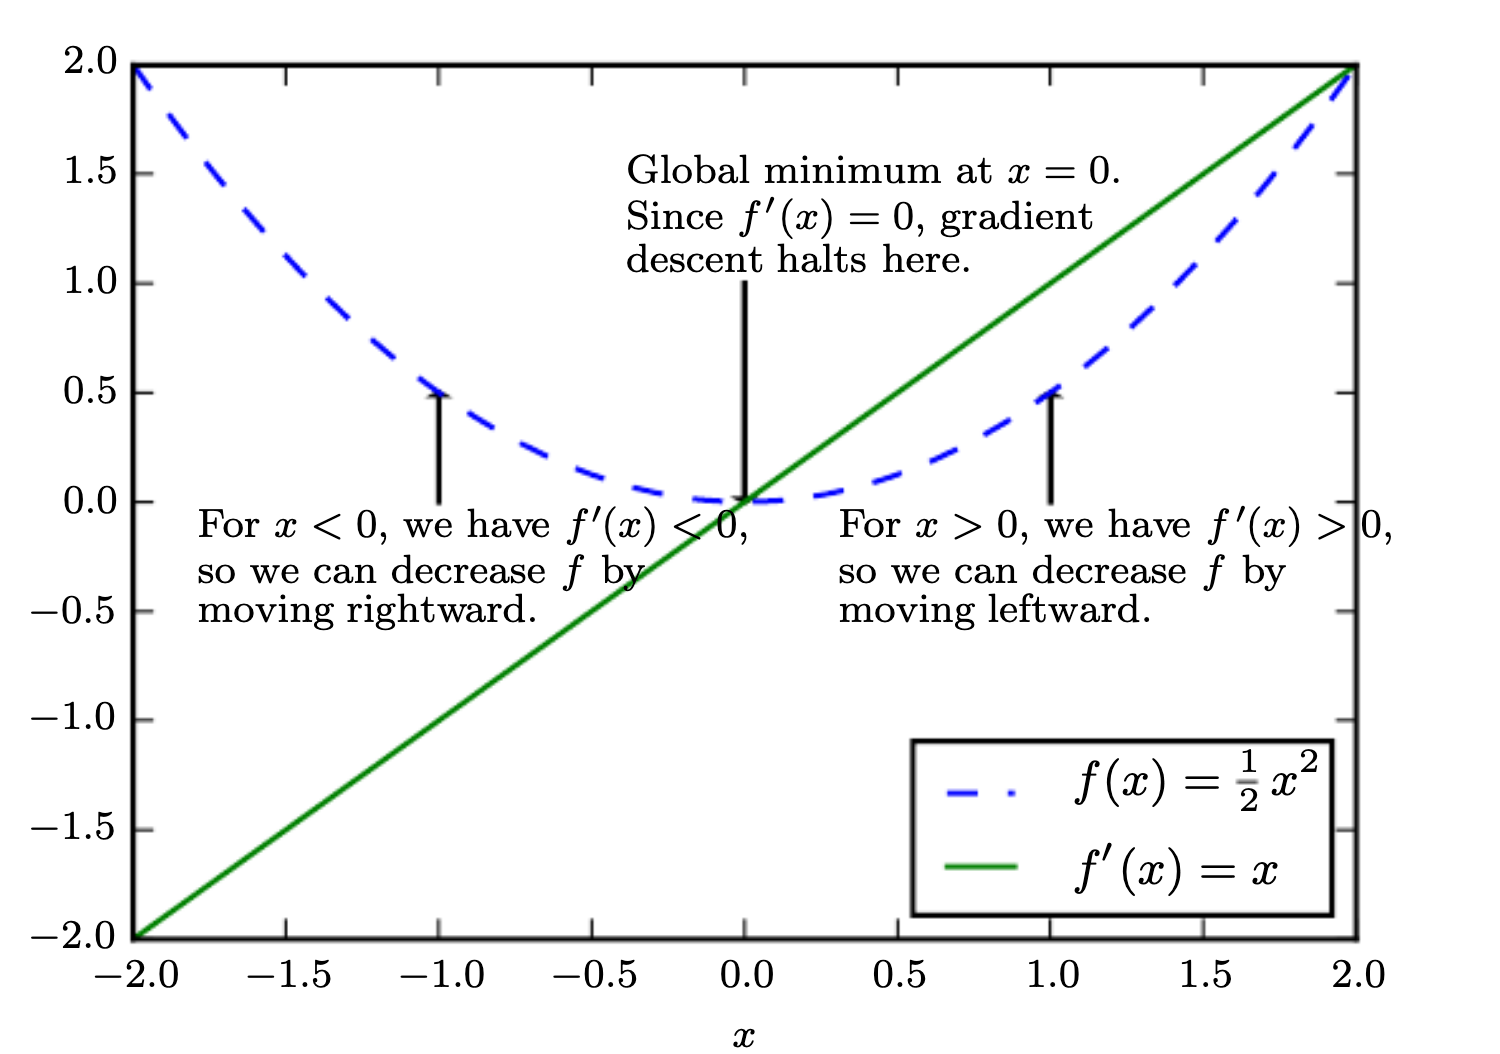
\includegraphics[scale=0.15]{chapters/assets/gradient_descent_basic.png}
    \caption{Gradient descent algorithm illustration for finding the minimum of a function $f(x) = \frac{1}{2}x^2$. Beginning with either positive of negative values of $x$, the gradient descent algorithm will find a minima at $x=0$ by moving in the direction opposite the sign of the gradient given by $f^\prime(x)=x$. Figure courtesy of \textcite{GoodfellowDLBook2016}.}
    \label{fig:gradient-descent}
\end{figure}

In \cref{fig:gradient-descent} the function $f(x)=\frac{1}{2}x^2$ depends only on the input $x$ and has a derivative \(f^\prime(x)=x\). In order to find the minimum of $f(x)$ we must find the value of $x$ where $f^\prime(x)=0$. The useful property of the gradient is that it tells us how to change $x$ to make a small change to $y$. For instance, we can infer that $f\left(x-\epsilon \operatorname{sign}\left(f^{\prime}(x)\right)\right) \ll f(x)$ for a small $\epsilon$. 
Therefore, to reduce $f(x)$, we can begin this process by starting with positive or negative values of $x$ and moving in the direction opposite to the sign of the gradient $f^\prime(x)$. The process is known as \textbf{gradient descent}, more specifically this update step reads:
\begin{align}
    x^\prime &=x-\epsilon \operatorname{sign}\left(f^{\prime}(x)\right) \nonumber \\
    &= x-\epsilon \operatorname{sign}\nabla_x f(x) \quad
\end{align}

\subsection{Backpropagation}\label{eqn:backprop}
The backpropagation as a learning algorithm was put forth by \textcite{rumelhart1986learning}, and is firmly based on the concept of gradient descent. We discussed gradient descent in the context of a simple function $f(x)$ that was dependent only on its input $x$, however, neural networks depend on the input $\symbfit{x}$ and a set of parameters $\symbfit{\theta}$, $f(\symbfit{x} \mathsemicolon \symbfit{\theta})$. Furthermore, the learning goal of neural networks is not to directly minimise the function $f(\symbfit{x} \mathsemicolon \symbfit{\theta})$. Rather, the goal of learning in neural networks is to minimise the cost function (or loss function) given the training set. 

Consider a network parameterised by $\symbfit{\theta} = \{\symbfit{w}, b\}$. The goal of backpropagation is to calculate partial derivatives \(\sfrac{\partial J}{\partial \symbfit{w}}\) and \(\sfrac{\partial J}{\partial b}\) of the cost function $J$ with respect to weight $\symbfit{w}$ and bias $b$. To further concretize the notion, we shall use the MSE loss from \Cref{sec:loss-fn}:
\begin{align}
    \mathcal{L}(\symbfit{\hat{y}}, \symbfit{y}) &= \frac{1}{2} \| \symbfit{y} - \symbfit{\hat{y}} \| ^ 2 \\
    J(\symbfit{\theta}) &= \frac{1}{2N} \sum_{i=1}^{N} \mathcal{L}(f(\symbfit{x} \mathsemicolon \symbfit{\theta}), \symbfit{y})
    \label{eqn:bp-cost-fn}
\end{align}
where $N$ is the total number of training samples. To calculate \(\sfrac{\partial J}{\partial \symbfit{w}}\) and \(\sfrac{\partial J}{\partial b}\), we apply the \textbf{chain rule} and calculate, in turn, the gradient of each intermediate variable and parameter. The first step is to calculate $\sfrac{\partial J}{\partial \mathcal{L}}$ which are the gradients of the cost function in \Cref{eqn:bp-cost-fn} with respect to the loss term $\mathcal{L}$.
Next, we must compute the gradient of the cost function with respect to the output variable $\symbfit{\hat{y}}$ according to the chain rule:
\begin{equation}
    \frac{\partial J}{\partial \symbfit{\hat{y}}}
= \frac{\partial J}{\partial \mathcal{L}} \times \frac{\partial \mathcal{L}}{\partial \symbfit{\hat{y}}}.
\end{equation}
Now we can calculate the gradient \(\sfrac{\partial J}{\partial \symbfit{w}}\), using the chain rule this yields:
\begin{equation}
    \frac{\partial J}{\partial \symbfit{w}}= \left(\frac{\partial J}{\partial \symbfit{\hat{y}}} \times \frac{\partial \symbfit{\hat{y}}}{\partial \symbfit{w}}\right).
\end{equation}
where \(\sfrac{\partial \symbfit{\hat{y}}}{\partial \symbfit{w}} = \symbfit{x}\).
Notice that the order of calculations are now \textbf{reversed} relative to those performed in the forward pass. Here we start with the output emitted by the neural network and work our way backwards towards the parameters. We can repeat the above steps for computing \(\sfrac{\partial J}{\partial b}\). Intuitively, this tells us how to update $\symbfit{w}$ and $b$ in order to reduce $J(\symbfit{\theta})$.

We must also be aware of the fact that we optimise for the loss function $\mathcal{L}$, that is, we are trying to find the optimal set of parameters $\symbfit{\theta}$ that will give us the lowest value of the loss function across $N$ training samples. In other words, we are trying to find the minima of $\mathcal L$ with respect to the input $\symbfit x$ and the parameters $\symbfit{\theta}$.
The gradient $\nabla_{\symbfit{\theta}}J$ across all samples is given as:
\begin{equation}
    \nabla_{\theta} J(\symbfit{\theta}) = \frac{1}{2N} \sum_{i=1}^{N}\nabla_{\symbfit{\theta}}\mathcal{L}(f(\symbfit{x};\symbfit{\theta}), y)
    % \bigg[\frac{\partial L}{\partial w}, \frac{\partial L}{\partial b}, \ldots \bigg]^\top
\end{equation}
where $\nabla_{\theta} J(\symbfit{\theta})$ is the average of the gradients of the loss function with respect to $\symbfit x$ and $\symbfit{\theta}$. The parameter update using the gradient descent algorithm with step size $\eta$ can be written as
\begin{equation}
    \label{eqn:basic-gd}
    \symbfit{\theta}^\prime=\symbfit{\theta}-\eta \nabla_{\theta} J(\symbfit{\theta}).
\end{equation}

However, this method is intractable for very large values of $N$. Therefore, we choose to compute gradients for a smaller set of $m$ samples such that $m \ll N$:
\begin{equation}
\label{eqn:sgd-proper}
    \nabla_{\theta} J(\symbfit{\theta}) = \frac{1}{2m} \sum_{i=1}^{m}\nabla_{\symbfit{\theta}}\mathcal{L}(f(\symbfit{x};\symbfit{\theta}), y).
    % \bigg[\frac{\partial L}{\partial w}, \frac{\partial L}{\partial b}, \ldots \bigg]^\top
\end{equation}
This is the idea of stochastic approximation behind \textbf{stochastic gradient descent} (SGD). It is an approximation of the gradient from a small number of input samples \parencite{Bottou2016}. The SGD update step in \cref{eqn:sgd-proper} is similar to \Cref{eqn:basic-gd}.
% \begin{equation}
% \symbfit{\theta}^{\prime}=\symbfit{\theta}-\eta \frac{1}{2m} \sum_{i=1}^{m} \nabla_{\symbfit{\theta}}J(\symbfit{\theta}).
% \end{equation}

Finally, for a network with $l$ layers, there are just as many gradients with respect to the loss function $\mathcal{L}$:
\begin{equation}
    \symbfit{\nabla_{\theta}} \mathcal{L}(f(\symbfit{x};\symbfit{\theta}), y) = \bigg[\frac{\partial \mathcal{L}}{\partial w^{(l)}}, \frac{\partial \mathcal{L}}{\partial b^{(l)}}, \frac{\partial L}{\partial w^{(l-1)}}, \frac{\partial \mathcal{L}}{\partial b^{(l-1)}}, \ldots, \frac{\partial \mathcal{L}}{\partial w^{(1)}}, \frac{\partial \mathcal{L}}{\partial b^{(1)}}\bigg]^\top
\end{equation}
where $\symbfit{\nabla_{\theta}} L(f(\symbfit{x};\symbfit{\theta}), y)$ is a vector of partial derivatives with respect to the weights in the neural network model while $w^{(l)}$ and $b^{(l)}$ are the weights and biases of layer $l$.

\import{chapters/}{02_basics_of_dl}

\import{chapters/}{03_conv_nets}

\newcommand{\mcG}{\mathcal{G}}
\newcommand{\mcV}{\mathcal{V}}
\newcommand{\mcE}{\mathcal{E}}
\newcommand{\bfitx}{\symbfit{x}}

\newcommand*{\ldblbrace}{\{\mskip-4mu\{}
\newcommand*{\rdblbrace}{\}\mskip-3mu\}}

\chapter{Basics of Geometric Deep Learning and Graph Neural Networks}\label{chap:gnn}

\section{Graphs}\label{sec:graphs}

In various branches of science, from biology to particle physics, graphs are often used as models of systems of relations and interactions. In this work, graphs are important as they engender a fundamental type of permutation invariance.

A basic \textbf{graph} \(\mcG=\left(\mcV, \mcE \right)\) is a collection of \textbf{nodes} $\mcV$ and \textbf{edges} \(\mcE\subseteq \mcV \times \mcV\) between pairs of nodes. Depending on the application or field, the nodes can also be called \textbf{vertices}, and the edges can be called \textbf{links} or \textbf{relations}.

For the purpose of an intuitive explanation, we assume that the nodes are associated with $s$-dimensional \textit{node features}, denoted by $\symbfit{x}_u$ for all $u \in \mcV$. Social networks are one of the most studied and best examples of graphs in the real world. Here, nodes represent users, edges correspond to friendship relations between them, and node features ($\symbfit{x}_u \in \mathbb{R}^d$) model user information such as age, location, last active time, etc. It should be noted that it is often possible to equip edges with features.
%however, this is not of concern within the scope of this work. Please refer to the detailed geometric deep learning text by \textcite{Bronstein2021}.


\begin{wrapfigure}{r}{0.25\textwidth}
    \centering
    % \captionsetup{justification=RaggedRight}
    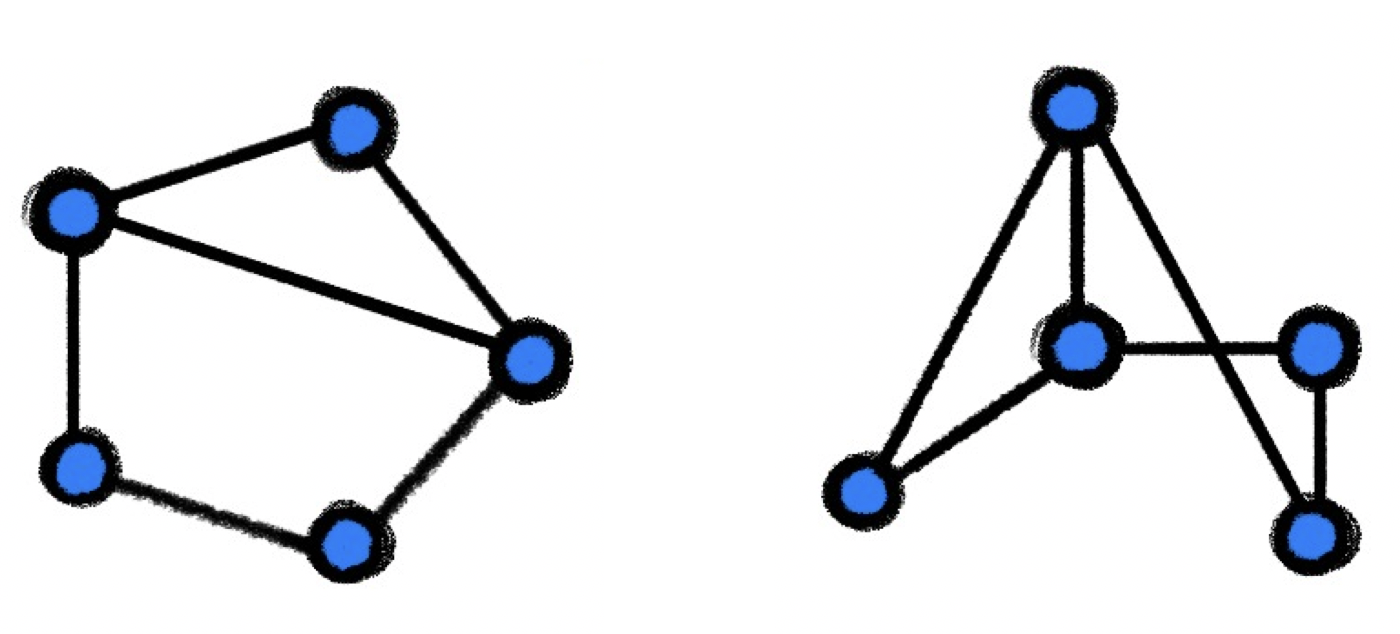
\includegraphics[scale=0.15]{chapters/assets/graph-figs/mn_isomorphic.png}
    \caption{Two isomorphic graphs}
    \label{fig:graph-isomorphism}
\end{wrapfigure}
A key property of graphs is that nodes in $\mcV$ are not typically assumed to be provided in any particular ordering, and thus, by extension, any operations performed on graph structures should not depend on any assumed inherent ordering of nodes. The desirable property that functions acting on graphs must possess is called \textbf{permutation invariance}, and implies that for any two \textbf{isomorphic} graphs, the results of such functions must be identical. {\em Isomorphism} is an edge-preserving bijection between two graphs. The two isomorphic graphs shown in \cref{fig:graph-isomorphism} are identical up to the reordering of their nodes.

Permutation invariance is important in \highlight[comment=add ref to article]{\samptr.} One of the main motivations behind \samptr\ is to allow the network to learn from multiple samples made available to the network in the form of a mini-batch. The ordering of the samples is of little interest to us as we are more concerned with learning by looking beyond single instances. The exact mechanism of this will be explained in more detail in subsequent sections.



\section{Janossy Pooling}\label{sec:janossy-pooling}
Let us first illustrate the concept of permutation invariance on \textbf{sets}, a special case of graphs without edges ($\mcE=\emptyset$). We illustrate this with the help of a framework provided to us in the form of Janossy pooling \parencite{Murphy2018}.

Currently, there are a few ways to incorporate permutation invariance. The first is the ``permute and average'' paradigm. It works by considering all possible permutations of input elements, then passing each permutation through a permutation-sensitive model or function, and then taking an average of all the results. If two inputs $\symbf{X}$ and $\Tilde{\symbf{X}}$ are permutations of each other, this process will give the same result for both inputs. Mathematically, this can be written as follows:
\begin{equation}
    \label{eqn:perm-invar-avg}
    \widehat{f}(\symbf{X}) = \frac{1}{|{T}_n|} \sum_{\pi \in {T}_n} \phi \bigl( \pi \left( \symbf{X} \right) \bigr)
\end{equation}
where $\symbf{X}=\left(\symbfit{x}_1, \ldots, \symbfit{x}_n\right)^\top$ is a stack of node features and has $n$ elements with $d$ dimensionality, $T_n$ is the set of all permutations of $n$ elements, and $\phi$ is a permutation-sensitive model. Therefore, we construct a permutation-invariant $\widehat{f}$ from a permutation-sensitive $\phi$.

This idea is called \textbf{Janossy pooling} and was first introduced by \textcite{Murphy2018}. Indeed, it is a straightforward and easy way to achieve permutation invariance, but it happens to be very computationally intensive. The computational cost is dominated by the sum over $T_n$ in \cref{eqn:perm-invar-avg}, where the number of elements in $T_n$ is $n!$. As one can imagine, if $\symbf{X}$ is a mini-batch with very large $n$, \cref{eqn:perm-invar-avg} quickly becomes intractable.

\begin{figure}[bh]
    \centering
    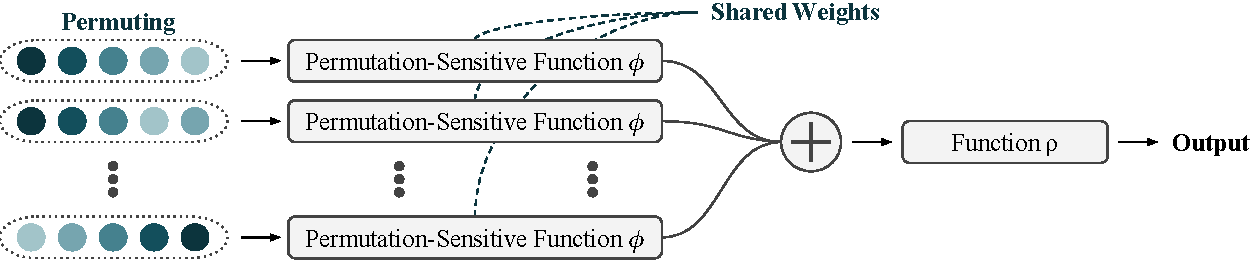
\includegraphics[width=\textwidth]{chapters/assets/graph-figs/permuting.pdf}
    \caption{$\widehat{f}$ comprises everything up to and including the sum. The function $\rho$ coming after the sum is optional and does not need to follow any constraints to guarantee invariance because its input, $\widehat{f}(x)$, is already invariant. Image courtesy of \textcite{wagstaff2022universal}.}
    \label{fig:basic-perm-invar}
\end{figure}
% \footnotetext{\url{https://fabianfuchsml.github.io/learningonsets}}

\subsection{A More Efficient Janossy Pooling}\label{ssec:efficient-janossy}

To save computational costs, we may give up the calculation of $n!$ permutations. In the above (\Cref{fig:basic-perm-invar}), we look at all possible $n$-tuples from the set of $n$ elements; instead, we can consider all $k$-tuples where $k \less n$ \parencite{Murphy2018}. We can then update \cref{eqn:perm-invar-avg} as:
\begin{equation}
    \label{eqn:k-tup-janossy}
    \widehat{f}(\symbf{X}) = \frac{1}{|P(n, k)|} \sum_{\symbf{X}_{\{k\}}} f(\symbf{X}_{\{k\}})
\end{equation}
where $\symbf{X}_{\{k\}}$ stands for a $k$-tuple of $\symbf{X}$.

Let us take a short example to understand how the count of values came about in \cref{eqn:k-tup-janossy}. Consider the input set ${w, x, y, z}$ with $n=4$. When we set $k=2$, then our sum will be applied over all $2$-tuples:
\[(w, x),~(x, w),(w, y),~(y, w),~(w, z),~(z, w),
(x, y),~(y, x),~(x, z),~(z, x),~(y, z),~(z, y)
\]
A sum over all these tuples is clearly invariant to permutations of elements in the input set, that is, each tuple appears exactly once in the sum no matter the order of individual elements. Therefore, the number of $k$-tuples from a set of $n$ elements is:
\begin{equation}
\label{eqn:k-tup-cnt}
    P(n,k) = \frac{n!}{(n-k)!}
\end{equation}

For $k \ll n$, this gives us a much more tractable method. Setting $k=n$ gives us the most expressive and most expensive model. Setting $k=1$ gives us a model whose cost is linear in the size of the input set. Increasing $k$ allows us to take into account higher-order interactions between elements in the set; we will come back to this idea of interactions in \Cref{ssec:relation-and-interactions}.

\begin{figure}[th]
    % \vspace{-0.2cm}
	\centering
% 	\hspace{-1cm}
	\begin{subfigure}[h]{0.46\textwidth}
		\centering
		\captionsetup{justification=centering}
		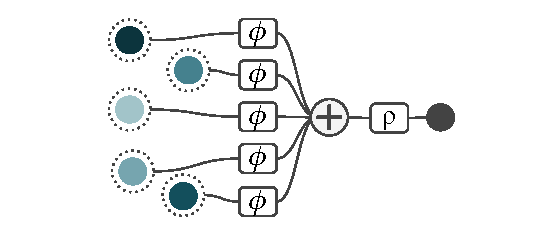
\includegraphics[width=0.99\textwidth]{chapters/assets/graph-figs/Janossy_K1.pdf}
		\caption{Janossy pooling with $k=1$ (\emph{Deep Sets})}
		\label{fig:Janossy_K1}
	\end{subfigure} 
	\begin{subfigure}[h]{0.46\textwidth}
		\centering
		\captionsetup{justification=centering}
		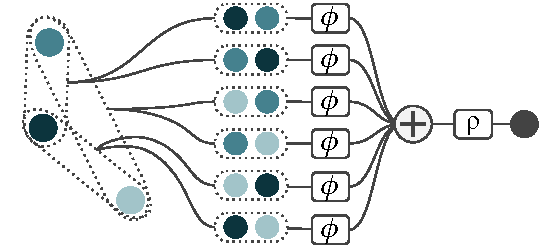
\includegraphics[width=0.99\textwidth]{chapters/assets/graph-figs/Janossy_K2.pdf}
		\caption{Janossy pooling with $k=2$}
		\label{fig:Janossy_K2}
	\end{subfigure} 
	\begin{subfigure}[h]{0.46\textwidth}
	    \vspace{+1cm}
		\centering
		\captionsetup{justification=centering}
		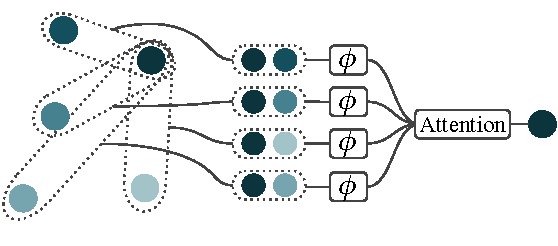
\includegraphics[width=0.99\textwidth]{chapters/assets/graph-figs/Janossy_K2Att.pdf}
		\vspace{-0.8cm}
		\caption{Self-attention}
		\label{fig:Janossy_K2Att}
	\end{subfigure} 
	\caption{Different variations of Janossy pooling. Permutation invariance is guaranteed by processing all combinations of $k$ elements and then aggregating via a sum (or softmax in the case of attention). Self-attention, a variant of Janossy pooling with $k=2$, focuses on one node at a time (the darkest node here), computing an output for this specific node. It is often employed for all nodes in parallel in a permutation-equivariant manner, mapping sets of points to sets of points \parencite{Lee2018}. Image borrowed from \textcite{wagstaff2022universal}.}
	\label{fig:k12}
\end{figure}

\subsection{Deep Sets}\label{ssec:deep-sets}

When $k=1$ and we include the optional function $\rho$, we obtain a popular special case known as Deep Sets \parencite{zaheer2017deep}. \citeauthor{zaheer2017deep} propose a neural architecture in which each input is first transformed by a neural network model $\phi$ individually (see \Cref{fig:Janossy_K1}), then the results are aggregated via a $\operatorname{sum}$ operator and further processed by a second neural network $\rho$.

The aforementioned functions produce a \textquote{global} graph-wise result, but we are frequently more interested in functions that work \textquote{locally} or node-wise. In order to acquire the collection of latent node features, for instance, we would wish to use some function to \textit{update} the features in each node. In other words, we may wish for a \textbf{node-wise} function to be permutation equivariant and want a permutation invariant \textbf{graph-wise} function.

We can now generalise the notions of permutation-invariance and equivariance from sets to graphs. In the generic setting $\mcE \neq \emptyset$, the graph connectivity can be represented by a $n \times n$ \textbf{adjacency matrix} $\symbf{A}$, defined as
\begin{equation}
    \label{eqn:adj-matrix-def}
    a_{u v}= \begin{cases}1 & (u, v) \in \mcE \\ 0 & \text { otherwise }.\end{cases}
\end{equation}

Note that now the adjacency and input (or feature) matrices $\symbf{A}$ and $\symbf{X}$ are \textquote{synchronised}, $a_{u, v}$
specifies the adjacency information between the nodes described by the $u\textsuperscript{th}$ and $v\textsuperscript{th}$
rows of $\symbf{X}$. Therefore, applying a permutation matrix $\symbf{P}$ to node features $\symbf{X}$ directly implies applying it to $\symbf{A}$'s rows and columns, $\symbf{PA}\symbf{P}^\top$. We then say that a graph-wise function $f$ is permutation invariant if 
\begin{equation}
    f\left(\symbf{P X}, \symbf{P A}^{\top}\right)=f(\symbf{X}, \symbf{A})
\end{equation}
and a node-wise function $\rho$ is permutation equivariant if
\begin{equation}
    \rho\left(\symbf{P X}, \symbf{P A P}^{\top}\right)=\symbf{P}\rho(\symbf{X}, \symbf{A})
\end{equation}

\subsection{Modelling Relations and Interactions}\label{ssec:relation-and-interactions}

\samptr\ has yet another fundamental idea that is essential for its success and operation. 
It is able to exploit the interactions (or relations) between elements in a set (mini-batch, which really means that we are trying to capture the fact that our model output may depend not only on the individual contribution of each element, but it may be crucial to also take into account the fact that certain elements appear together in the same set. Our goal is simply to model and use these interactions.

To illustrate this with a simple example, imagine the task of evaluating how well a set of ingredients work together to cook a meal. Setting $k=1$ allows the function $\phi$ to consider related individual attributes, but it cannot detect conflicts between ingredients (e.g., garlic vs. vanilla). Larger $k$ allows $\phi$ to see more than one item at a time, allowing it to make relational inferences about pairs of ingredients, allowing for a more expressive model of deliciousness. Considering $\phi$ as an encoder and $\rho$ as a decoder, $\phi$ can encode information about interactions, which $\rho$ can use for decoding.

Similar to the above example, $\samptr$ uses \highlight[comment=cite/ref here]{contrastive learning} in order to learn to place semantically similar images closer together in an embedding space. When we increase $k$, we give our model the expressivity to learn to recognise semantic similarities between images and to explicitly take these relations into account. By allowing the model to consider relations between images in a mini-batch, it can better decide which images belong closer together in the feature space and in turn learn better discriminative semantic features. Bear in mind that the image is first passed through a CNN (see \Cref{chap:cnn}), and all the other operations explained here are applied to the flattened output of the CNN.


\section{Janossy Pooling and Self-Attention}\label{sec:jan-attn}

Many of the current neural architectures resemble Janossy pooling with $k=2$.
\textbf{Self-attention} \parencite{vaswani2017attention} is one such algorithm that is also used in the context of graphs in \samptr. Self-attention works by comparing two elements of a set at a time, usually by performing a scalar product.
The results of the scalar products are used as \textbf{attention weights} to aggregate information from different points using a weighted permutation invariant sum. Although it is similar to binary Janossy pooling, self-attention also uses $\operatorname{softmax}$ to ensure that attention weights sum up to $1$ (see \Cref{sec:softmax}).

To substantiate the relationship between permutation-invariant binary Janossy pooling and self-attention, we first define a natural extension of $k$-ary Janossy pooling from permutation \textit{invariance to equivariance}. In normal binary Janossy pooling, the function $\phi$ acts on every two-tuple, followed by the $\operatorname{sum}$-pooling operation. For the purpose of visualisation and intuition, we will write these two-tuples as a matrix:
\begin{equation}
    \begin{bmatrix}
    \phi(\bfitx_1, \bfitx_1) & \phi(\bfitx_2, \bfitx_1) & \cdots & \phi(\bfitx_n, \bfitx_1) \\
    \phi(\bfitx_1, \bfitx_2) & \phi(\bfitx_2, \bfitx_2) & \cdots & \phi(\bfitx_n, \bfitx_2) \\
    \vdots                   &  \vdots              & \ddots & \vdots         \\
    \phi(\bfitx_1, \bfitx_n) & \phi(\bfitx_2, \bfitx_n) & \cdots & \phi(\bfitx_n, \bfitx_n)
    \end{bmatrix}
    \label{eqn:jan-attn-matrix}
\end{equation}

If we pool over the \textit{entire matrix} we get an invariant output. However, pooling over \textit{each row individually} we get a permutation equivariant output.
In general, we define $k$-ary equivariant Janossy pooling as follows: the $i\textsuperscript{th}$ output is obtained by aggregating the overall ($\phi$-transformed) $k$-tuples which start with the element $\bfitx_i$. A second network $\rho$ may then further transform each output individually. Mathematically, this reads:
\begin{equation}
    f_i(\symbf{x}) = \rho \left( \sum_j \phi(\bfitx_i, \bfitx_j) \right).
    \label{eqn:janossy-attention}
\end{equation}

In practise, however, the process is slightly more involved. Typically, $\phi(\bfitx_i, \bfitx_j)$ is divided into \textbf{attention weights} $w(\bfitx_i, \bfitx_j)$ and \textbf{values} $v(\bfitx_j)$ and a softmax is applied on the attention weights. Furthermore, the attention weights themselves would be born from the scaled dot-product between two affine transformations called the \textbf{query} and \textbf{key}.
However, the elegant view from the lens of binary Janossy pooling remains clear. We shall come back to self-attention and its usage in $\samptr$ in later sections.

\section{Graph Neural Networks}\label{sec:graph-nn}

Now that we have described graphs and permutation invariant and equivariant functions, we can begin to talk about Graph Neural Networks (GNNs). GNNs are perhaps among the most \textbf{general} class of deep learning architectures in existence at this moment. Some deep learning architectures can be understood as special cases of the GNN with additional geometric structure. As it happens, we have already covered one such specific case, self-attention in \cref{sec:jan-attn}.

Notice that in \Cref{sec:jan-attn}, the output of $i\textsuperscript{th}$ depends on all pairs of $(i, j)$. However, we can also constrain this so that the $i\textsuperscript{th}$ output is more dependent on \textbf{local} nodes. This means that instead of considering all pairs, the output of node $i$ instead depends on a smaller set of neighbours. We can formalise this to define what we mean when a node is a  \textquote{neighbour} of another node.

The \textbf{neighbourhood} of $i$ is defined as:
\begin{equation}
\mathcal{N}_{i}=\{j:(i, j) \in \mathcal{E} \text { or }(j, i) \in \mathcal{E}\}
\end{equation}
and the neighbourhood features as the multiset:
\begin{equation}
\symbf{X}_{\mathcal{N}_{i}}=\ldblbrace\bfitx_{j}: j \in \mathcal{N}_{i}\rdblbrace .
\end{equation}

Further generalising on our perspective developed in \Cref{sec:janossy-pooling} and \Cref{sec:jan-attn}, we can specify a function $\varphi(\bfitx_i, \symbf{X}_{\mathcal{N}_{i}})$ that is locality aware and can operate over a node and its neighbourhood. Then a permutation equivariant function $h$ can be constructed by applying $\varphi$ to every node's neighbourhood separately:
\begin{equation}
    h({\symbf X}, {\symbf A}) =
\left[
  \begin{array}{ccc}
     & \varphi(\bfitx_1, \symbf{X}_{\mathcal{N}_1}) &  \\
     & \varphi(\bfitx_2, \symbf{X}_{\mathcal{N}_2}) &  \\
             & \vdots    &          \\
     & \varphi(\bfitx_n, \symbf{X}_{\mathcal{N}_n}) & 
  \end{array}
\right].
\label{eq:graph_equivariant}
\end{equation}

As $h$ is constructed by applying a shared function $\varphi$ to each node locally, its permutation equivariance rests on the output of $\varphi$ being independent of the ordering of the nodes in $\mathcal{N}_i$. Therefore, if $\varphi$ is built to be permutation invariant, then this property will be satisfied. Observe that the role $\varphi$ plays here is that of $\widehat{f}$ in \Cref{eqn:perm-invar-avg} and role played by $h$ is similar to that of $f$ in \Cref{eqn:janossy-attention}.

\begin{figure}[th]
    \centering
    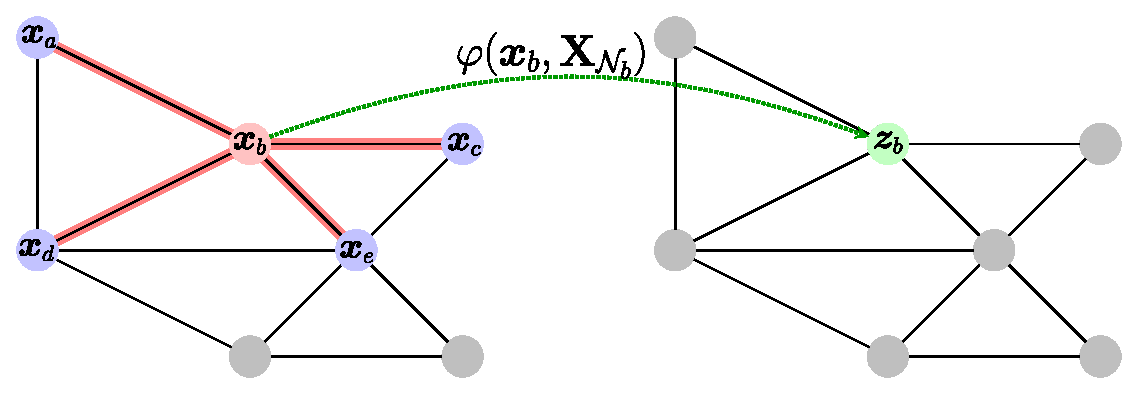
\includegraphics[width=\linewidth]{chapters/assets/graph-figs/GC_GDL.eps}
    \caption{By applying a permutation-invariant function $\varphi$ to every neighbourhood. In this case, $\varphi$ is applied to the features $\bfitx_b$ of node $b$ as well as the multiset  of its neighbourhood features, $\symbf{X}_{\mathcal{N}_b} = \ldblbrace\bfitx_a, \bfitx_b, \bfitx_c, \bfitx_d, \bfitx_e\rdblbrace$. Applying $\varphi$ in this manner to every node's neighbourhood recovers the rows of the resulting matrix of latent features $\symbf{Z}=h(\symbf{X}, \symbf{A})$. Image modified from \parencite{Bronstein2021}.}
    \label{fig:gc_gdl}
\end{figure}%

A GNN is a optimisable transformation on the attributes of a graph (nodes, edges, global-context) that preserves permutation invariance.
Based on our discussion in \Cref{ssec:deep-sets}, we consider a graph to be specificed with an adjacency matrix $\symbf{A}$ and node features $\symbf{X}$. We will discuss GNN architectures that are \textbf{permutation equivariant} functions $h(\symbf{X}, \symbf{A})$ constructed by applying shared permutation invariant functions $\varphi(\bfitx_i, \symbf{X}_{\mathcal{N}_i})$ where $\symbf{X}_{\mathcal{N}_i}$ is the neighbourhood of $\bfitx_i$. This local function $\varphi$ can be referred to as \textquote{diffusion}, \textquote{propagation}, or \textquote{message-passing}, and the over computation $h$ is referred to as a GNN layer.

\begin{figure}
    \centering
    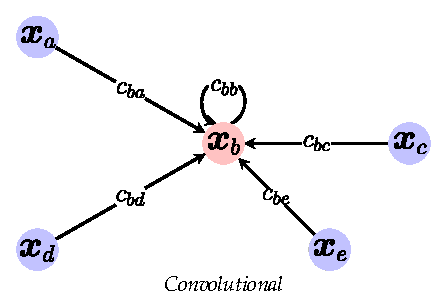
\includegraphics[width=0.33\linewidth]{chapters/assets/graph-figs/GNN_GDL_TYPES_C.eps}
    \hspace{-0.5em}
    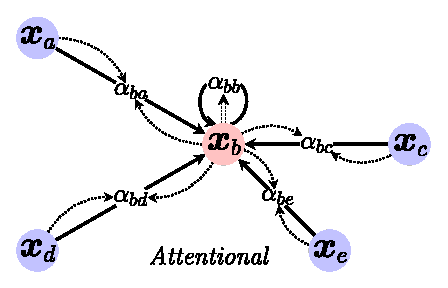
\includegraphics[width=0.33\linewidth]{chapters/assets/graph-figs/GNN_GDL_TYPES_A.eps}
    \hspace{-0.5em}
    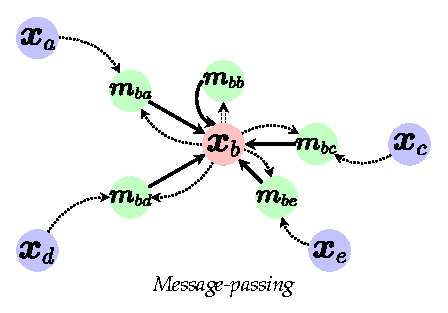
\includegraphics[width=0.33\linewidth]{chapters/assets/graph-figs/GNN_GDL_TYPES_MP.eps}
    \caption{A visualisation of the dataflow for the three flavours of GNN layers, $g$. We use the neighbourhood of node $b$ from Figure \ref{fig:gc_gdl} to illustrate this. Left-to-right: \textbf{convolutional}, where sender node features are multiplied with a constant, $c_{uv}$; \textbf{attentional}, where this multiplier is \emph{implicitly} computed via an attention mechanism of the receiver over the sender: $\alpha_{ij}=a(\vec{x}_i, \vec{x}_j)$; and \textbf{message-passing}, where vector-based messages are computed based on both the sender and receiver: $\vec{m}_{ij}=\psi(\vec{x}_i, \vec{x}_j)$.}
    \label{fig:gc_flavours}
\end{figure}%

There are three types of GNN layers that are most common, in all three of them permutation invariance is satisfied by \textbf{aggregating} features from $\symbf{X}_{\mathcal{N}_i}$ (potentially transformed by another function $\psi$) with some permutation-invariant function $\bigoplus$, and then \textbf{updating} the features of node $i$, by means of some function $\varphi$. Usually, $\varphi$ and $\psi$ are learnable affine transformations with activation functions (see \Cref{chap:basics-of-dl}) and $\bigoplus$ is an operation such as $\operatorname{sum}$, $\operatorname{mean}$, or $\operatorname{max}$. These operations are analogous to pooling functions discussed in \Cref{sec:conv-pooling}.

In the \textbf{convolutional} kind of GNNs \parencite{kipf2016semi}, the features of the neighbourhood nodes are directly aggregate with fixed weights,
\begin{equation}
    z_{u}=\varphi\left(\bfitx_{i}, \bigoplus_{j \in \mathcal{N}_{i}} c_{i j} \psi\left(\bfitx_{j}\right)\right).
    \label{eqn:gcn}
\end{equation}
Here, $c_{ij}$ specifies the importance of node $i$ to node $j$'s representation.

In the attentional scheme \parencite{velic018graph, brody2021attentive}, the interactions are implicit
\begin{equation}
z_{i}=\varphi\left(\bfitx_{u}, \bigoplus_{j \in \mathcal{N}_{i}} a\left(\bfitx_{i}, \bfitx_{j}\right) \psi\left(\bfitx_{j}\right)\right)
\label{eqn:attn-gnn}
\end{equation}
Here, $a$ is a learnable \textbf{self-attention} mechanism that computes the importance coefficients $\alpha_{ij} = a(\bfitx_i,\bfitx_j)$ implicitly. They are often softmax-normalised across all neighbours. If the aggregation operation $\bigoplus$ is summation, then the aggregation is a linear combination of the neighbourhood node features, but the weights are feature-dependent. The reader is urged to recognise the similarities between \Cref{eqn:attn-gnn} and \Cref{eqn:janossy-attention}.

Finally, the \textbf{message-passing} type amounts to computing arbitrary vectors (\textquote{messages}) across edges,
\begin{equation}
    z_{i}=\varphi\left(\bfitx_{i}, \bigoplus_{j \in \mathcal{N}_{i}} \psi\left(\bfitx_{i}, \bfitx_{j}\right)\right)
    \label{eqn:mesg-passing}
\end{equation}
Here, $\psi$ is a learnable message function, computing $j$'s vector sent to $i$, and the aggregation can be considered as a form of message passing on the graph.

It must be noted that the relationship between the three approaches is as follows, \textit{convolution} $\subseteq$ \textit{attention} $\subseteq$ \textit{message-passing}. The attentional mechanism can represent convolutional GNNs by an attention-mechanism implemented as a lookup table $a(\bfitx_i, \bfitx_j) = c_{ij}$. Message-passing can represent both convolutional and attentional GNNs where the messages are only the sender node's features: $\psi(\bfitx_i, \bfitx_j)=c_{ij}\psi(\bfitx_j)$ for convolutional GNNs and $\psi(\bfitx_i, \bfitx_j)=a\left(\bfitx_{i}, \bfitx_{j}\right)\psi(\bfitx_j)$ for attentional GNNs. $\samptr$ makes use of the attentional semantics in the message-passing context to implement its GNN, however the implementation of the attention mechanism follows \parencite{vaswani2017attention} instead of the mechanism suggested in \parencite{velic018graph}.

\chapter{Self Supervised Learning} \label{chap:self-supervised-learning}

In recent years, the field of artificial intelligence has progressed leaps and bounds at an astronomical rate. 
However, the vast majority of progress has been made in the \textbf{supervised} domain, where we have massive amounts of carefully labelled data available. Such models perform extremely well in the singular task for which they were trained.

However, the reality is such that we cannot always possess massive amounts of labelled data for a given task at hand.
There are some tasks for which there are simply not enough high-quality labelled data. Examples of such tasks include modelling esoteric languages for which we do not have enough resources or several image classification tasks in the medical domain.
Furthermore, supervised learning has shown us that it is constrained when it comes to building easily generalisable models.
If AI systems can gain a more nuanced understanding of the reality beyond what is specified and constrained by training labels, they will ultimately be closer to human-level understanding.
\begin{figure}[th]
    \centering
    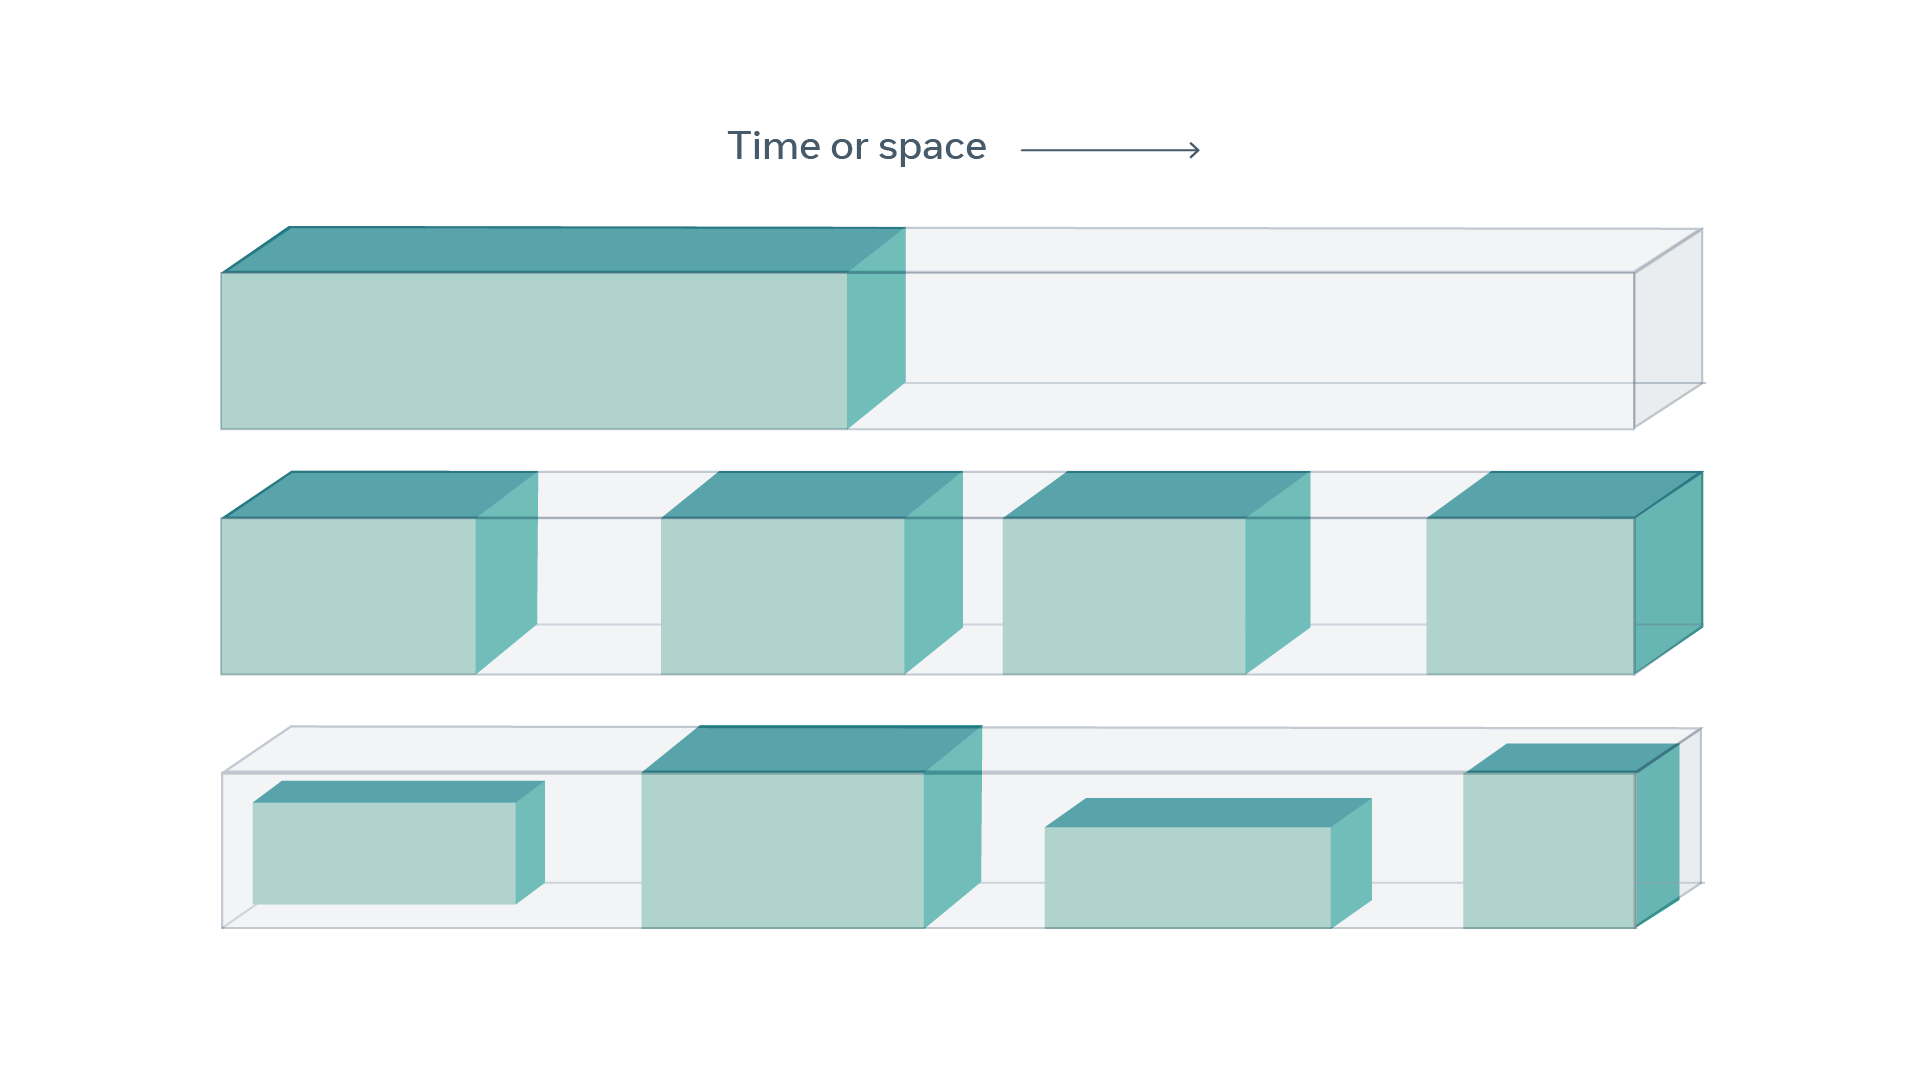
\includegraphics[width=\linewidth]{chapters/assets/ssl_figs/ssl.png}
    \caption{In self-supervised learning, the system is trained to predict hidden parts of the input (in \textcolor{gray}{gray}) from visible parts of the input (in \textcolor{tudelft-turquoise}{green}).}
    \label{fig:ssl-idea}
\end{figure}

Self-supervised learning (SSL) is currently the most promising form of \textbf{unsupervised learning} alternative to supervised learning, which is perhaps capable of guiding AI systems to learn general knowledge and an approximate form of common sense. Self-supervision typically involves formulating a specialised supervised task to predict only a subset of information from the rest (see \Cref{fig:ssl-idea}). This idea has been used extensively in language modelling. The default task of a language model is to predict the next word given a sequence of words (or a partial sentence). We then use the trained model to help us solve another related task. This concept is called \textbf{transfer learning}, where we the \textbf{pre-train} the model on a large dataset, then save the weights and apply it to another possibly related problem. The pre-training can be either supervised or unsupervised; however, we shall only be focusing on the unsupervised (self-supervised) aspect. It is also worth noting that most self-supervised training schemes focus on \textbf{representation learning}, and we shall cover this in a bit more detail in \Cref{sec:repr-learning}.

SEER \parencite{Goyal2021}, a research project from Meta AI, made use of SWaV \parencite{caron2020unsupervised} to train a computer vision model that has outperformed state-of-the-art supervised models on tasks such as image classification, object detection, and image segmentation. SEER's performance demonstrates quite conclusively that SSL methods can excel at computer vision tasks while learning generalisable features. The work done on SEER parallels the work being done in the NLP field for a while now, where state-of-the-art models frequently use billions of parameters and train using SSL methods on huge datasets.


\section{Representation Learning} \label{sec:repr-learning}
The performance of machine learning methods is highly dependent on the choice of data representation (or features) on which they are applied. For that reason, much of the actual effort in deploying machine learning algorithms goes into the design of preprocessing pipelines and data transformations that result in a representation of the data that can support effective machine learning. Our goal with representation learning is to allow the model to learn robust representations with minimal human interference.

Representation learning aims to train machine learning algorithms to learn useful representations, e.g. interpretable representations, useful latent features, or allow transfer learning to be used. 
Deep neural networks can be considered representation learning models that typically encode information which is projected into a different subspace. These representations are then usually passed on to a linear classifier to, for instance, train a classifier. 
\begin{figure}[h]
    \centering
    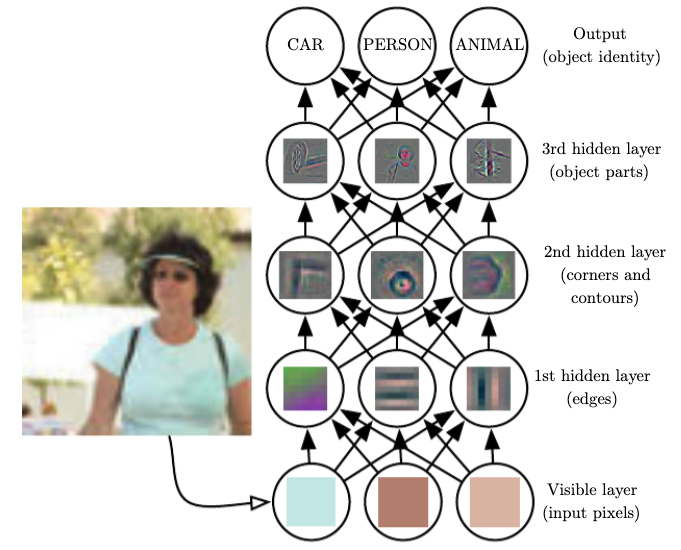
\includegraphics[scale=0.4]{chapters/assets/ssl_figs/ssl_rep_learning_images.png}
    \caption{Deep neural networks combine simple concepts to learn representations and derive complex structures in a hierarchical pipeline. Each layer refines  information from the previous layer. Finally, the  classifier takes the transformed representation and draws boundaries between classes. See \Cref{fig:feature-viz} for more.}
    \label{fig:small-cnn-features}
\end{figure}

At a high level, a network has two components:
\begin{enumerate}
    \item an encoder (also called a feature extractor in \Cref{fig:cnn-overview})
    \item and a linear classifier.
\end{enumerate}
The encoder transforms the input data and projects them into a subspace that we refer to as \textbf{latent space}. Then the representation (output of the encoder) is passed to a linear classifier. Typically, in a supervised setting, we would like to map representations to labels, which a classical classifier would do. 
However, representation learning aims to map representations to other representations. These learned representations are often dense and compact; they can also generalise to similar data modalities. In other words, these representations can \textbf{transfer} well to other tasks and have been the principal method for solving problems in which data annotations are hard or even impossible to get. The learned representations are stored in the weights of the model, \Cref{fig:small-cnn-features} shows a small example where the hidden layers have learnt to recognise specific components of an image. One can save these learnt weights and reuse them for other tasks. 

\section{Self-supervision with Images} \label{sec:self-sup-with-images}

\begin{figure}
    \centering
    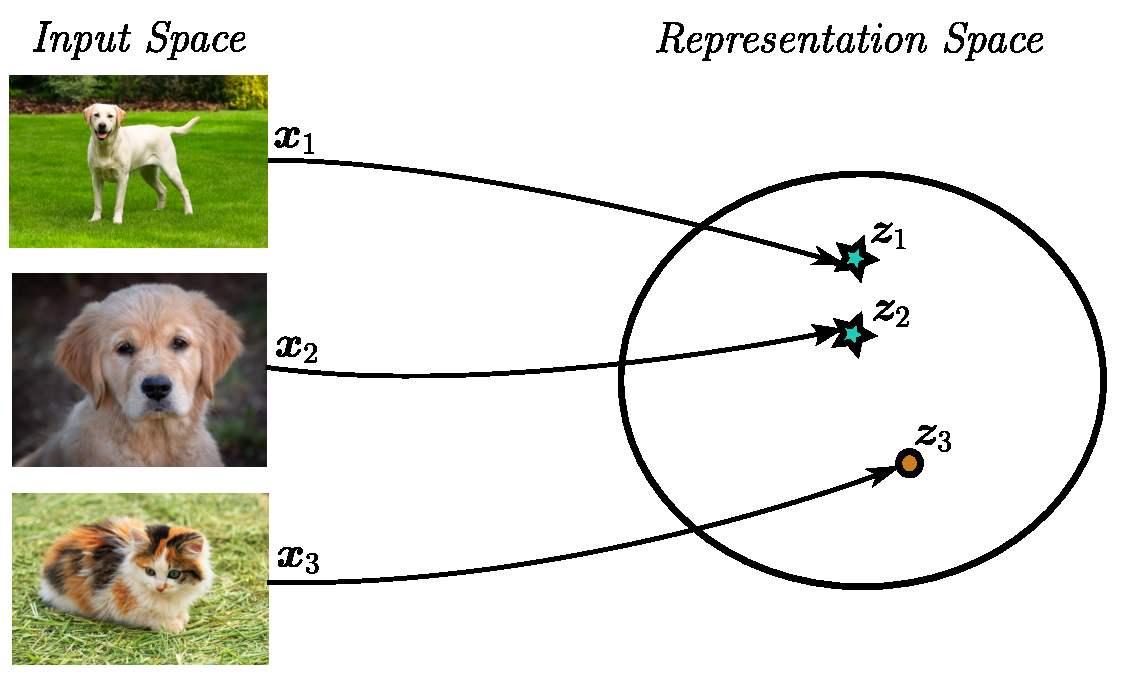
\includegraphics[scale=0.4]{chapters/assets/ssl_figs/representation_space.pdf}
    \caption{We have three images $\symbfit{x}_1, \symbfit{x}_2$ and $\symbfit{x}_3$. The first two images depict a dog, and the third image depicts a cat. The network should ideally learn to place the dogs closer together ($\symbfit{z}_1$ and $\symbfit{z}_2$) in the representation space and the cat ($\symbfit{z}_3$) farther away from the dogs.}
    \label{fig:my_label}
\end{figure}

As mentioned above in this text, self-supervision usually involves formulating a specialised supervised task; this task is also called a \textbf{pre-text task}. However, we normally do not care about the performance of the model on this artificial task. Rather we are more concerned with the intermediate learned representations with the hope that this representation carries with it good semantic or structural meanings that be beneficial to a wide variety of real word tasks.

For example, we might rotate images at four random angles and train a model to predict how each image has been rotated. Here, the task of predicting rotations is the pre-text task, so the actual accuracy on this task is irrelevant to us \parencite{gidaris2018unsupervised}. Instead, we expect the model to learn high-quality latent representations that are useful for other real-world tasks.

However, this is not the only way, and in the next section we shall discuss one of the most popular techniques in this space.

\section{Contrastive Representation Learning}\label{sec:contrastive-learning}
The goal of contrastive representation learning is to learn a feature subspace in which similar (positive) pairs of data items stay close to each other while dissimilar (negative) pairs are farther apart. Contrastive learning can be applied to both supervised and unsupervised settings. For unsupervised learning, contrastive learning remains one of the most powerful approaches to self-supervised learning.

When working in the supervised setting, it is easy to mine for positive pairs of the data; one only needs to fetch images that are associated with the same true label. However, in an unsupervised setting, we have no such label information, therefore we must get creative in order to teach the network what constitutes as a positive pair of images. This brings us to one of the most intuitive techniques, SimCLR \parencite{chen2020simple}.

\subsection{SimCLR} \label{ssec:simclr}

\begin{figure}[th]
\centering
\begin{subfigure}{.19\textwidth}
  \centering
  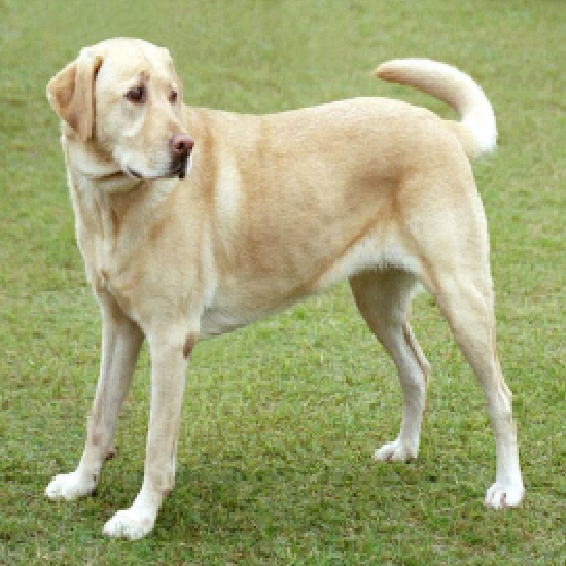
\includegraphics[width=0.9\linewidth]{chapters/assets/ssl_figs/transforms/img_original.pdf}
  \caption{Original}
\end{subfigure}\begin{subfigure}{.19\textwidth}
  \centering
  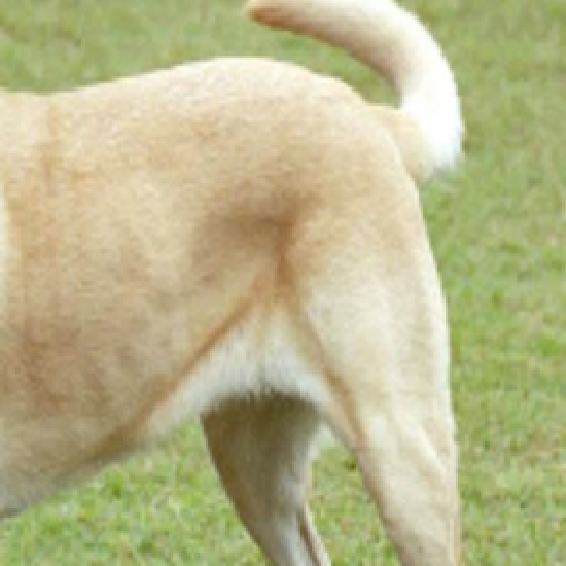
\includegraphics[width=0.9\linewidth]{chapters/assets/ssl_figs/transforms/img_crop1.pdf}
  \caption{Crop and resize}
\end{subfigure}\begin{subfigure}{.19\textwidth}
  \centering
  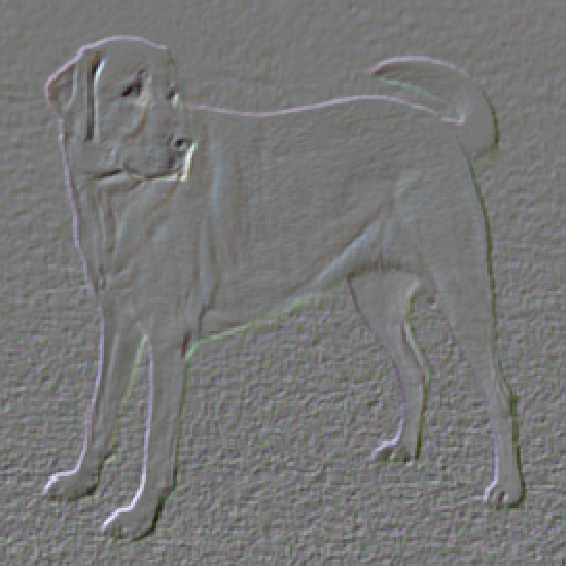
\includegraphics[width=0.9\linewidth]{chapters/assets/ssl_figs/transforms/img_sobel.pdf}
  \caption{Sobel filtering}
\end{subfigure}\begin{subfigure}{.19\textwidth}
  \centering
  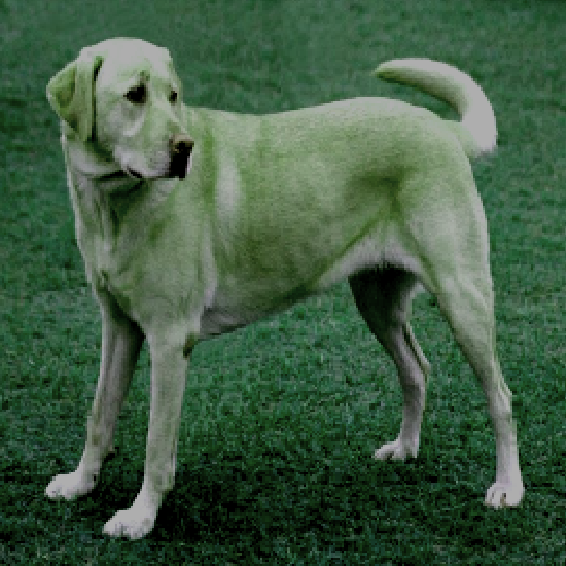
\includegraphics[width=0.9\linewidth]{chapters/assets/ssl_figs/transforms/img_color1.pdf}
  \caption{Color distort. (drop)}
\end{subfigure}\begin{subfigure}{.19\textwidth}
  \centering
  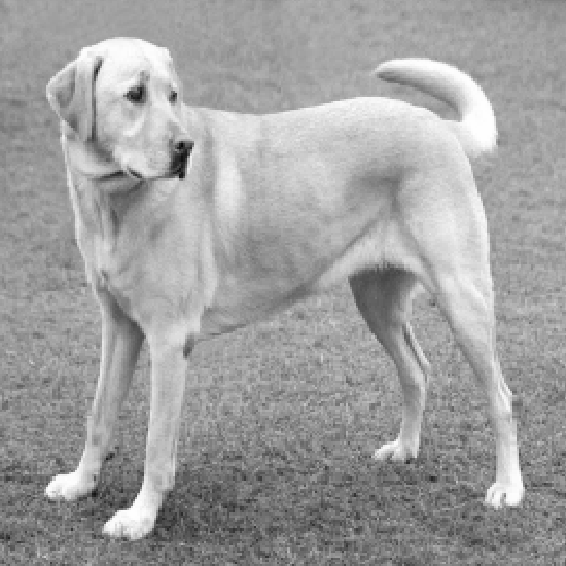
\includegraphics[width=0.9\linewidth]{chapters/assets/ssl_figs/transforms/img_color.pdf}
  \caption{Color distort. (jitter)}
\end{subfigure}\\
\begin{subfigure}{.19\textwidth}
  \centering
  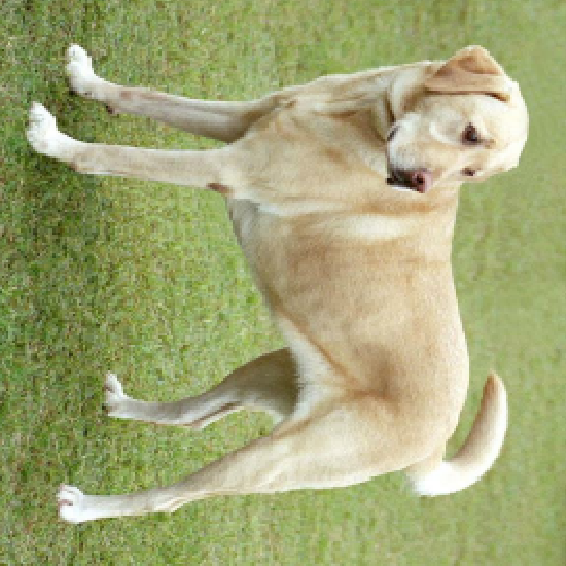
\includegraphics[width=0.9\linewidth]{chapters/assets/ssl_figs/transforms/img_rotate.pdf}
  \caption{Rotate {\tiny$\{90\degree,180\degree,270\degree\}$}}
\end{subfigure}\begin{subfigure}{.19\textwidth}
  \centering
  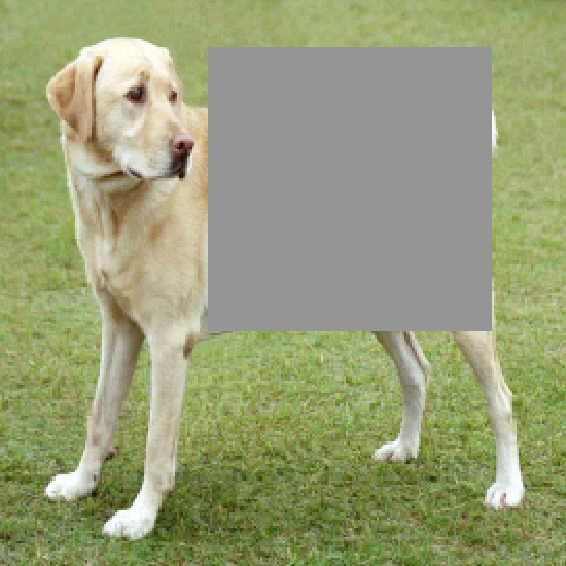
\includegraphics[width=0.9\linewidth]{chapters/assets/ssl_figs/transforms/img_cutout.pdf}
  \caption{Cutout}
\end{subfigure}\begin{subfigure}{.19\textwidth}
  \centering
  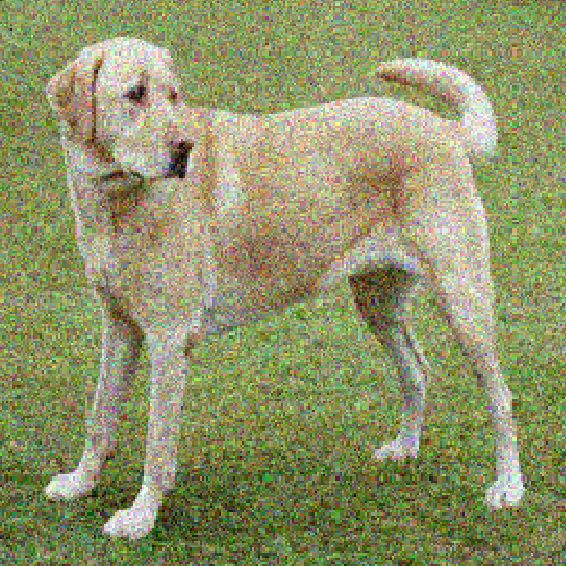
\includegraphics[width=0.9\linewidth]{chapters/assets/ssl_figs/transforms/img_noise.pdf}
  \caption{Gaussian noise}
\end{subfigure}\begin{subfigure}{.19\textwidth}
  \centering
  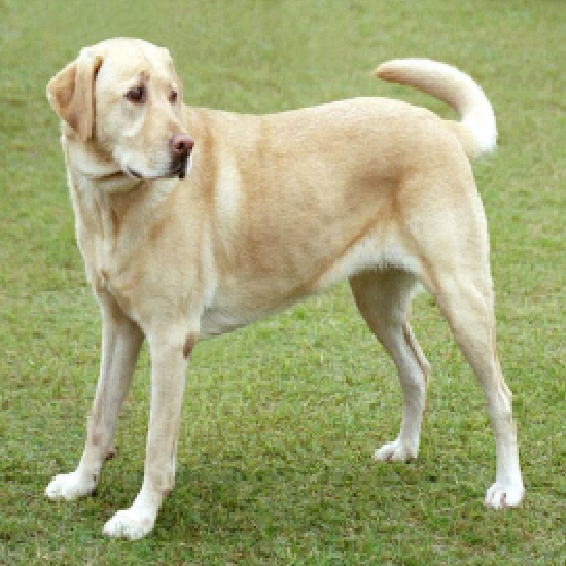
\includegraphics[width=0.9\linewidth]{chapters/assets/ssl_figs/transforms/img_gblur.pdf}
  \caption{Gaussian blur}
\end{subfigure}\begin{subfigure}{.19\textwidth}
  \centering
  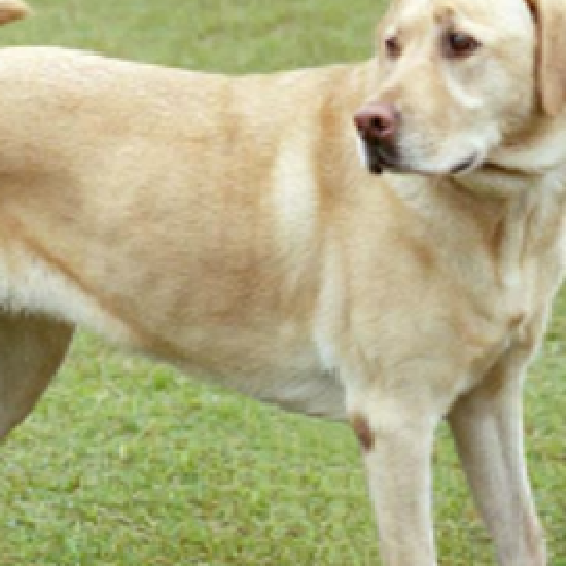
\includegraphics[width=0.9\linewidth]{chapters/assets/ssl_figs/transforms/img_crop.pdf}
  \caption{Crop, resize (and flip)}
\end{subfigure}\vskip -0.05in
\caption{Illustrations of data augmentation operators. (Original image cc-by: Von.grzanka)}
\label{fig:simclr-data_aug}
\end{figure}

The idea behind SimCLR is quite simple and elegant. An image $\symbfit{x}$ is randomly sampled from the dataset, and then two random transformations are applied to the image to get two augmented images $\symbfit{x}_i$ and $\symbfit{x}_j$. Each image is passed through the encoder to obtain the representations $\symbfit{z}_i$ and $\symbfit{z}_j$, respectively. The goal here is to maximise the similarity between $\symbfit{z}_i$ and $\symbfit{z}_j$, see \Cref{fig:simclr} for a small overview of SimCLR. \Cref{fig:simclr-data_aug} shows a few examples of the type of image transformations used by SimCLR.

In order to train the network to bring the said representations closer, we first measure the similarity between them using a \textbf{similarity metric} such as cosine similarity or Euclidean distance. The cosine similarity metric between $\symbfit{z}_i$ and $\symbfit{z}_j$ is given as
\begin{equation}
\label{eqn:simclr-cosine-sim}
s_{i, j}=\frac{\symbfit{z}_{i}^{\top} \symbfit{z}_{j}} {\left(\left\|\symbfit{z}_{i}\right\|\left\|\symbfit{z}_{j}\right\|\right)}
\end{equation}

\highlight[comment=maybe add an example of the mini batch]{We} calculate the pairwise cosine similarity between each augmented image in a mini-batch using \Cref{eqn:simclr-cosine-sim}. In the ideal case, the similarity between all \textit{postive} pairs must be high and low between all \textit{negative} pairs.

Next, we use the pairwise cosine similarities to calculate the loss. The loss is called \textbf{NT-Xent} (normalised temperature-scaled cross-entropy loss) or NCE (noise contrastive estimator) and is given as
\begin{equation}
\ell(i, j)=-\log \frac{\exp \left(s_{i, j} / \tau\right)}{\sum_{k=1}^{2 n} \mathbb{1}_{[k \neq i]} \exp \left(s_{i, k} / \tau\right)}
\label{eqn:nt-xent}
\end{equation}
where $\tau$ is the temperature scaling factor. The reader is urged to recognise the similarities between \Cref{eqn:nt-xent} and \Cref{eqn:std-softmax}. \Cref{eqn:nt-xent} is indeed just the normal $\operatorname{softmax}$ (\Cref{eqn:std-softmax}) with an additional temperature scaling factor.

Normally a mini-batch of $n$ samples is randomly sampled, since the contrastive pretext task is defined on pairs of augmented images derived from the minibatch, it results in a total of $2n$ data points. The negative samples are not sampled explicitly. Instead, given a positive pair, the other $2(n-1)$ augmented samples in a mini-batch are treated as negative samples.

You can choose $\tau$ to be any value; higher values of $\tau$ will lead to a \textquote{softer} output distribution of probabilities, for example, $\left[0.01,0.01,0.98\right]$.
As $\tau$ approaches $0$, it will lead to a distribution \textquote{sharper}, for example, $\left[0.2,0.2,0.6\right]$.
A distribution of \textquote{softer} implies that the model is less confident in its predictions, while \textquote{sharper} implies that the model is very confident.

A low temperature ($<1$) discourages predictions from collapsing to a uniform distribution, which is undesirable. When we talk about collapse, we are talking about \textbf{representation collapse}. Representation collapse is a phenomenon where in the network outputs the same representation regardless of the input, as one can imagine if every pair of images has the same representation, the loss would be incredibly low. However, if the network returns the same representation for all input, its not very useful for downstream tasks that require the features to be discriminative and have semantic information.

\begin{tcolorbox}[title=Intuition for Temperature]
The temperature parameter penalises the larger logits more than the smaller logits. The exponential function is an \textquote{increasing function}. So, if a term is already large, penalising it by a small amount would make it much smaller (\% wise) than if that term were small.
\end{tcolorbox}

\begin{figure}
    \centering
    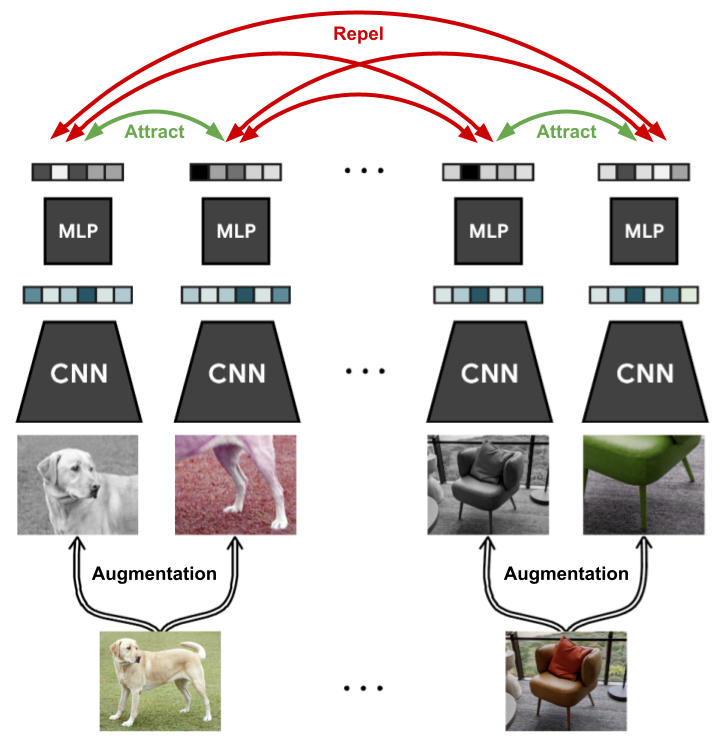
\includegraphics[scale=0.4]{chapters/assets/ssl_figs/simclr_contrastive_learning.png}
    \caption{SimCLR works by augmenting an image twice and ensuring their representations are close to each other while being farther away from representations of other augmented images.}
    \label{fig:simclr}
\end{figure}

\newcommand{\mcQ}{\mathcal{Q}}
\newcommand{\mcS}{\mathcal{S}}
\newcommand{\mcT}{\mathcal{T}}
\newcommand{\mcD}{\mathcal{D}}
\newcommand{\nwks}[2]{${#1}$-way, ${#2}$-shot}

\chapter{Few-Shot Learning}\label{chap:fsl}
A good machine learning model often requires training with a large number of samples. Humans, on the contrary, learn new concepts and skills much faster and more efficiently. Children who have only seen cats and birds a few times can quickly tell them apart. People who know how to ride a bike are likely to discover how to ride a motorcycle quickly with little or even no demonstration. Is it possible to design a machine learning model with similar properties - learning new concepts and skills fast with a few training examples? That is essentially what few-shot learning is designed to solve.

Despite notable advances in the field of artificial intelligence, two essential aspects of human conceptual intelligence have consistently eluded machine learning and artificial intelligence (AI) systems. 
First, for most interesting kinds of natural and man-made categories of entities, humans can learn a new concept from just one or a few handful examples, whereas many AI models would require several thousands of examples to perform satisfactorily. 
Second, people learn far richer representations than machines do, even for seemingly simple concepts, and use them for a wide variety of tasks such as creating new entities based on the exemplars, classifying objects into parts, grasping between concepts and parts, and creating new abstract categories (concepts) by combining existing ideas and concepts.
In contrast to this, the best machine learning models and neural networks cannot perform these additional functions using their specialised learnt representations. 
The challenge arises when we wish for AI models to learn new concepts and representations from few examples and ensure that these representations are abstract and flexible.

To tackle this challenge, few-shot classification is cast as a task of predicting class labels for a set of unlabelled data points (\textit{query set}) given only a small set of labelled data points (\textit{support set}). Typically, the query and support data points are drawn from the same distribution. 

Few-shot classification methods typically consist of two sequential phases: (i) \textit{pre-training} on a large dataset of \textquote{base} classes, regardless of whether the training is supervised or unsupervised. This is followed by (ii) \textit{fine-tuning} on an unseen dataset consisting of \textquote{novel} classes. Normally, the classes used in the pre-training and fine-tuning are mutually exclusive. In this paper, our focus is on the self-supervised (also sometimes interchangeably called \textquote{unsupervised} in the literature) setting where we have no access to the actual class labels of the \textquote{base} dataset.

To this end, various methods have been proposed and broadly categorised under two different approaches:
\begin{itemize}
    \item \textbf{Meta-learning}. Where an algorithm \textquote{learns how to learn} and aims to find a quickly generalisable model
    \item \textbf{Transfer Learning}. Where the model is trained to learn optimal representations that are generalisable with minimal updates
\end{itemize}

The first approach, \textit{meta-learning}, relies on episodic training that involves creating synthetic \textquote{tasks} to mimic the downstream episodic fine-tuning phase \parencite{Finn2017Model-agnosticNetworks, Hsu2018UnsupervisedMeta-Learning, Khodadadeh2018UnsupervisedClassification, Antoniou2019AssumeAugmentation, Ye2022, lee2021meta, Ji2019UnsupervisedTraining}. 
The second method follows a \textit{transfer learning} approach, where the network trained non-episodically to learn optimal representations in the pre-training phase, which is then followed by an episodic fine-tuning phase \parencite{Medina2020Self-SupervisedClassification, goodemballneed2020, dhillon2019baseline}.
In this method, a feature extractor (encoder) is trained using a form of metric learning to capture the structure of the unlabelled data. 
Next, a simple predictor (conventionally a linear layer) is utilised in conjunction with the pre-trained feature extractor for quick adaptation to the novel classes in the fine-tuning phase.
The better the feature extractor captures the global structure of the unlabelled data, the less the predictor requires training samples and the faster it adapts itself to the unseen classes in the fine-tuning phase (also the testing phase).

% Furthermore, supervised approaches that follow the episodic training paradigm may include a certain degree of \textit{task awareness}.
% Such approaches exploit the information available in the query set during the training or testing phases \parencite{bateni2022enhancing, ye2020few, Cui2021} to alleviate the model's sample bias. As a results of this, task-awareness allows the model to learn task-specific embeddings by better aligning the features of the support and query samples.
We also see a set of supervised approaches that do not rely purely on a convolutional feature extractor. Instead, these approaches also make use of graphs and graph neural networks \parencite{garcia2018fewshot, kim2019edge, yu2022hybrid, yang2020dpgn}. Using a graph neural network (GNN) can help in modelling instance-level and class-level relationships. GNN's can also help propagate labels by using a task-agnostic classifier, and such methods have been shown to work quite effectively compared to their standard convolutional counterparts \parencite{kim2019edge, garcia2018fewshot, yu2022hybrid, yang2020dpgn}. However, graph-based methods have eluded the unsupervised setting.

Several recent studies have questioned the necessity of meta-learning for few-shot classification \parencite{goodemballneed2020, Medina2020Self-SupervisedClassification, dhillon2019baseline, ziko2020laplacian, boudiaf2020information,chen2021self}. They report competitive performance on few-shot benchmarks without episodic training or few-shot task-based experiences during training. These methods follow the second approach and aim to solve the few-shot learning problem by fine-tuning a pre-trained feature extractor with a standard cross-entropy loss.
Some of these methods \parencite{Medina2020Self-SupervisedClassification, goodemballneed2020, das2022confess} in the space demonstrate that the transfer learning approach outperforms meta-learning based methods in standard in-domain and cross-domain settings - where the training and novel classes come from totally different distributions.

\section{Formalising the Few-Shot Learning Problem}\label{sec:formalising-fsl}

In a few-shot setting, the model aims to generalise well and quickly enough on a variety of new and potentially unseen tasks after being trained for optimal performance on various learning tasks.
Each task is associated with a dataset $\mathcal{D}$, containing both inputs and true labels. 
The model parameters of an optimal generalisable model are defined as follows:
\begin{equation}
    \symbfit{\theta}^\star = \arg\min_{\symbfit \theta} \mathbb{E}_{\mathcal{D}\sim \pdata} [\mathcal{L}_{\symbfit \theta}(\mathcal{D})]
\end{equation}

First, we look at how \(\mathcal{D}\) is structured in a standard supervised few-shot setting. 
Consider a labelled dataset of size $M$, $\mathcal{D} = \{({\symbfit x}_i, y_i)\}_{i = 1}^{M}$ of images $\symbfit{x}_i$ and class labels $y_i$. 
This dataset $\mathcal{D}$ is divided into three disjoint subsets: $\left\{\mathcal{D}_\textup{tr}\, \cup\, \mathcal{D}_\textup{val}\, \cup\, \mathcal{D}_\textup{tst}\right\} \in \mathcal{D}$, referring to the training, validation, and test subsets, respectively.

Next, we define a set of randomly sampled tasks $\mathcal{T}_i$ drawn from the training dataset $\mathcal{D}_{\textup{tr}} = \{({\symbfit x}_i, y_i)\}_{i = 1}^{M^\textup{tr}}$ of size $M^\textup{tr}$. A task $\mathcal{T}_i$ consists of two parts: (i) the support set $\mathcal{S}$ form which the model learns, (ii) the query set $\mathcal{Q}$ on which the model is evaluated. The support set $\mathcal{S}$ is constructed by drawing $K$ labelled random samples from $N$ different classes resulting in the so-called ($N$-way, $K$-shot) settings.
Therefore, each task $\mathcal{T}_i$ is made up of a $\textit{support}$ and a $\textit{query}$ set, $\mcT_i=\langle \mcS, \mcQ \rangle$, and each task can also be referred to as an \textquote{episode}. Any given task contains $NK$ support and $NQ$ query images, respectively, that are mutually exclusive.
% This dataset $\mathcal{D}$ is divided into three disjoint subsets: $\left\{\mathcal{D}^\textup{tr}\, \cup\, \mathcal{D}^\textup{val}\, \cup\, \mathcal{D}^\textup{test}\right\} \in \mathcal{D}$, respectively, referring to the training, validation, and test subsets. The validation dataset $\mathcal{D}^\textup{val}$ is used for model selection and the testing dataset $\mathcal{D}^\textup{test}$ for final evaluation. The episodic training is carried out on a set of tasks $\mathcal{T}_i \sim p(\mathcal{T})$. 
% Every \textquote{task} is a self-contained learning problem, each relying on small \textquote{support} and \textquote{query} sets to mimic the few-shot circumstances encountered during evaluation.
% The tasks are constructed by drawing $K$ random samples from $N$ different classes, which we denote as an ($N$-way, $K$-shot) task. 
\begin{figure}[ht]
    \centering
    \captionsetup{justification=centering}
    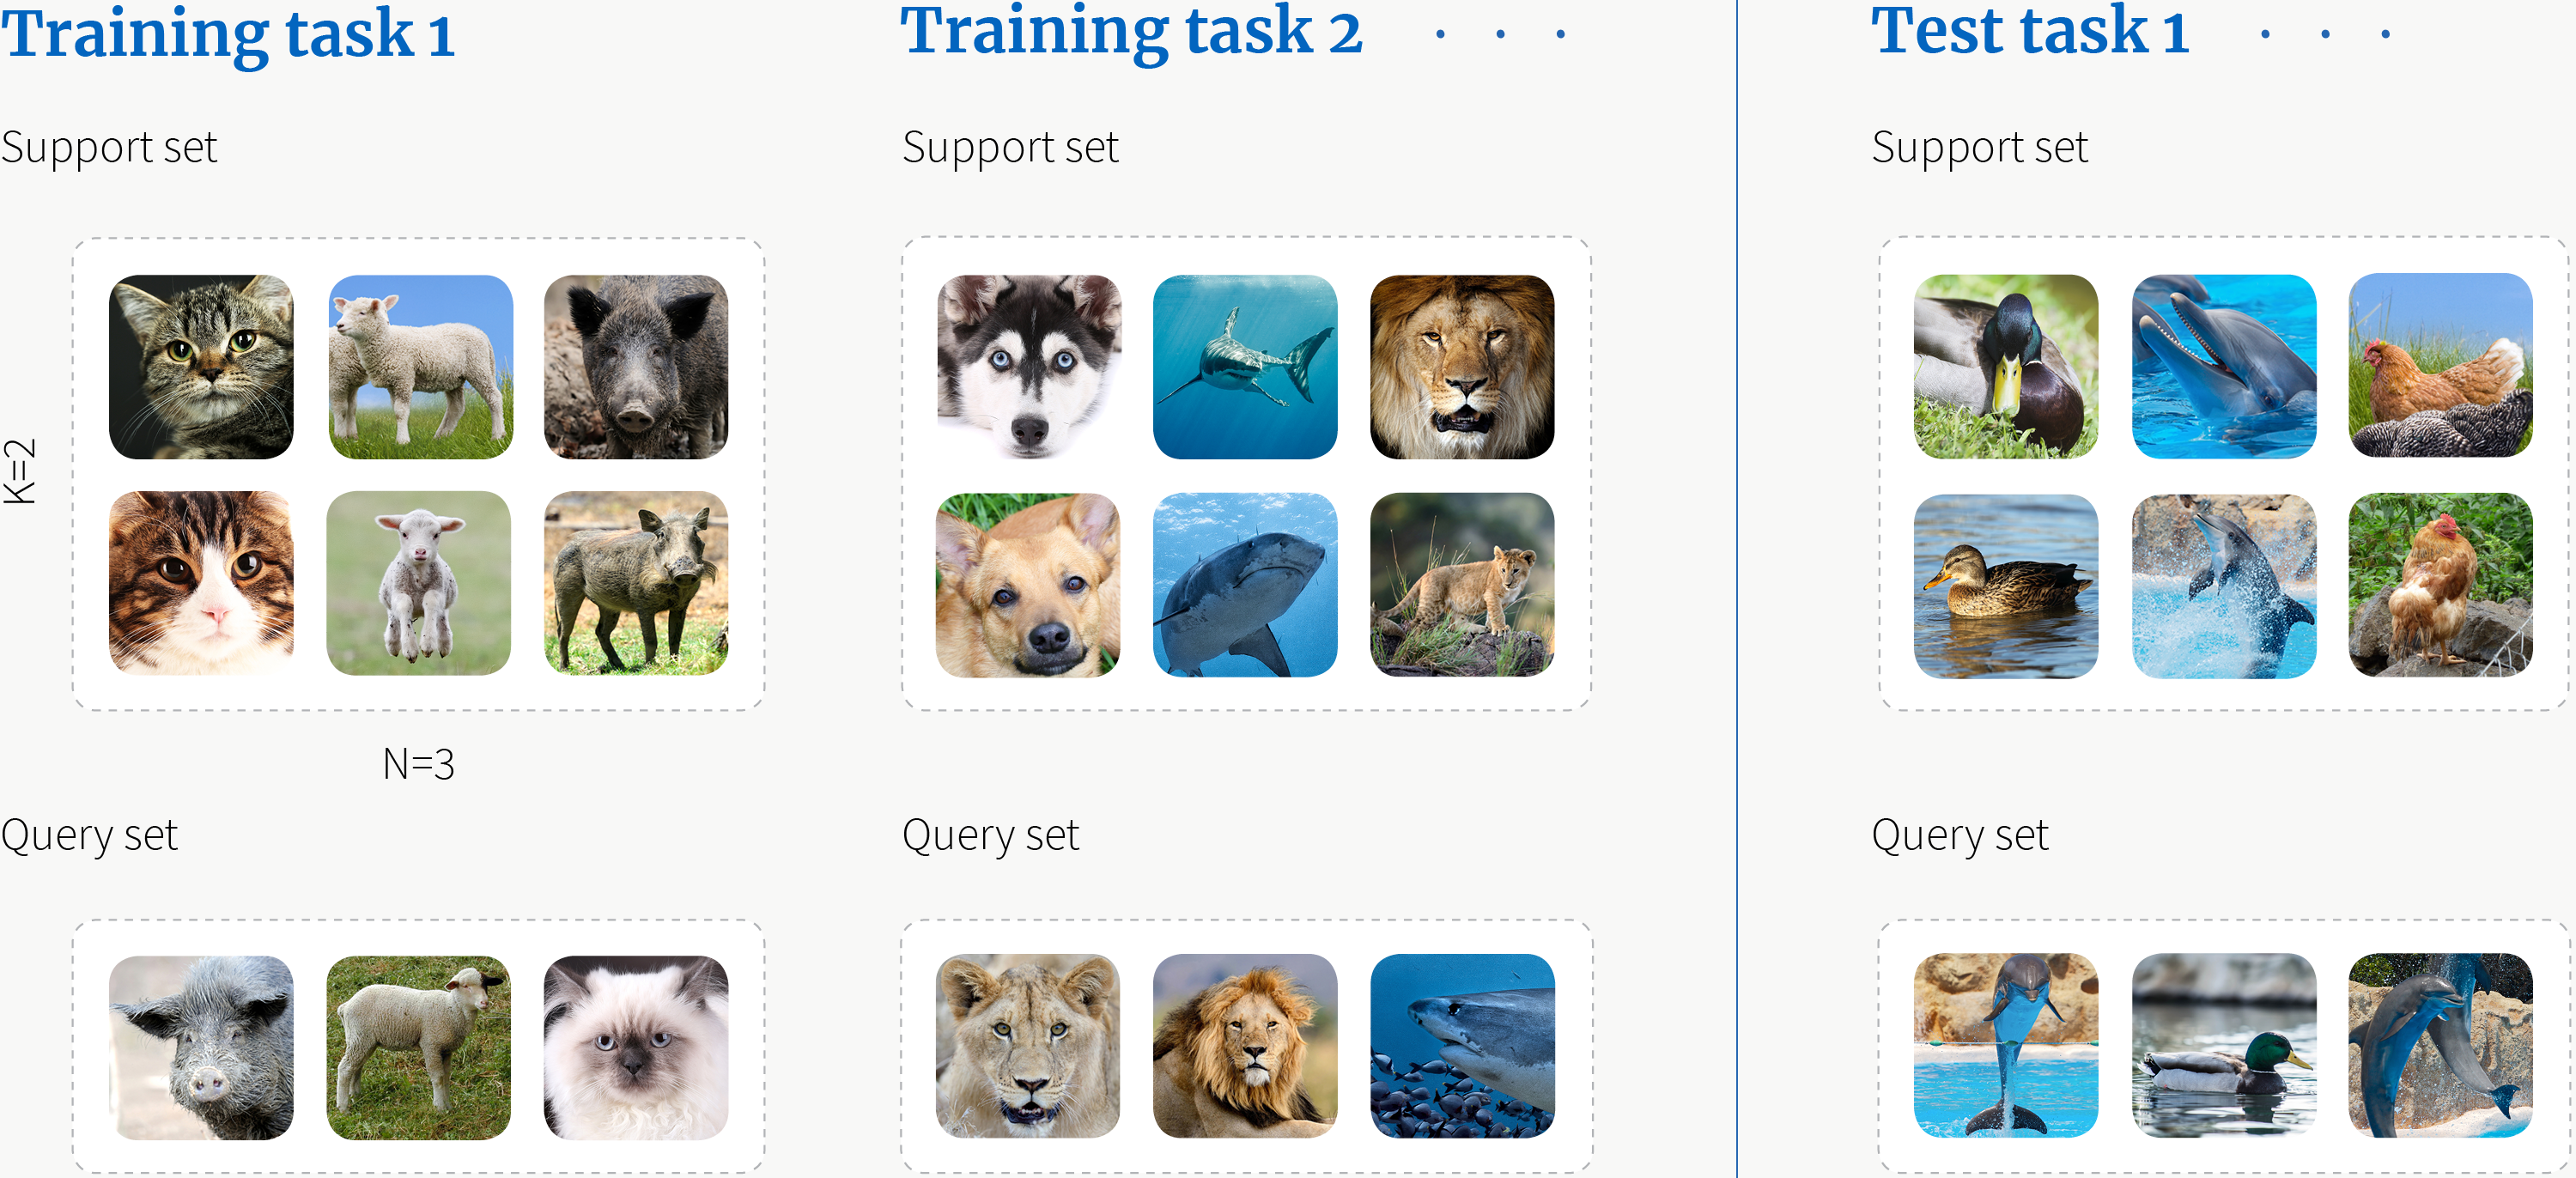
\includegraphics[width=\linewidth]{chapters/assets/fsl/n3k2.png}
    \caption{An example of (\nwks{3}{2}) image classification.}
    \label{fig:fsl-tasks}
\end{figure}

In most training routines, tasks are randomly sampled from a task distribution based on the training subset $\mcD_\textup{tr}$ of the dataset $\mcD$ according to the (\nwks{N}{K}) setting, and then the model parameters are updated by back-propagation after each task is processed.
This comprises one \textbf{episode}. The model is expected to quickly learn the optimal parameters from the $NK$ support data points and apply the learnt weights to classify the $NQ$ unlabelled query data points, on which performance is evaluated.
\Cref{fig:fsl-tasks} shows (\nwks{3}{2}) training tasks, it should be noted that even during testing (downstream classification task) the model is presented with tasks that are in the same (\nwks{3}{2}) form as the training tasks.

\section{Model Agnostic Meta Learning (MAML)}\label{sec:maml}


\begin{wrapfigure}{r}{0.25\linewidth}
    \centering
    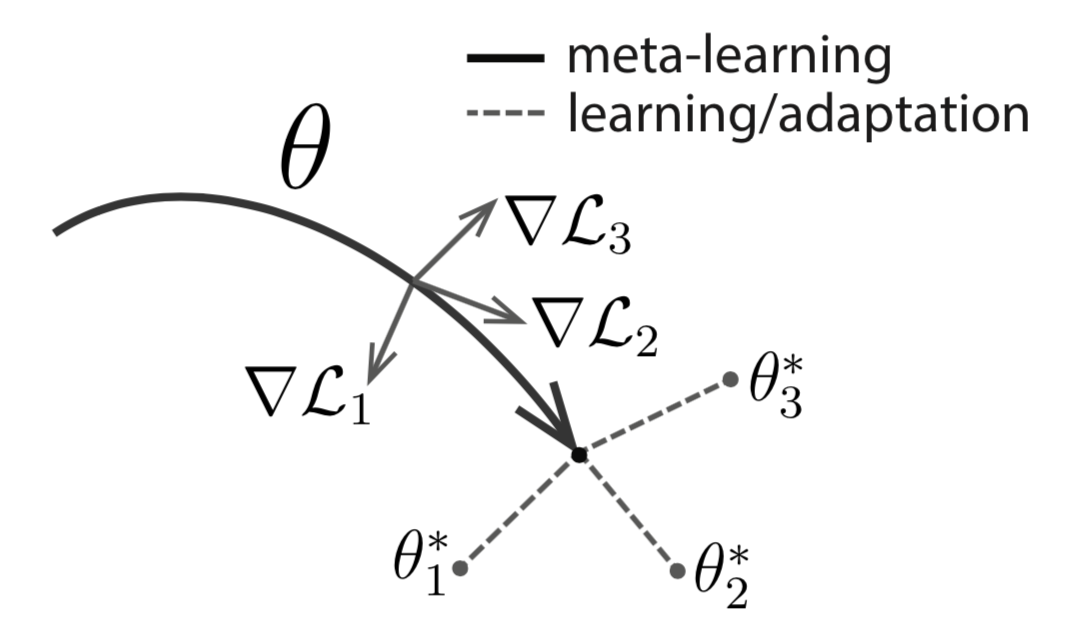
\includegraphics[scale=0.23]{chapters/assets/fsl/maml.png}
    \caption{MAML tries to find optimal generalised weights, by first finding optimal weights in the inner learning phase.}
    \label{fig:maml}
\end{wrapfigure}
\textbf{Meta-learning} is most commonly understood as \textquote{learning to learn}, which refers to the process of improving a learning algorithm over multiple learning episodes and was first proposed by \textcite{schmidhuber:1987:srl}. On the contrary, conventional ML improves model predictions on multiple data instances. 
During base learning, an \emph{inner} learning algorithm solves a task such as image classification, defined by a dataset and an objective. During meta-learning, an \emph{outer} algorithm updates the inner learning algorithm so that the model it learns improves an outer objective.
The learning episodes of the base task, namely tuples of the image $\bfitx_i$ and associated label $y_i$, can be seen to provide the instances that the outer algorithm needs to learn the base learning algorithm

MAML is a gradient-based \textbf{meta learning} method. It is a technique that works with any model that learns through gradient descent. It trains a model to find an optimal set of weights that can be quickly adapted to a new task, through a few gradient descent steps. The meta-learner tries to find an initial set of weights that are not only useful for adapting to various problems, but also can be adapted quickly (in a small number of steps) and efficiently (using only a few examples).
\Cref{fig:maml} illustrates how MAML should work at meta-test time. We are looking for a pre-trained parameter that can reach near-optimal parameters for every task in one or a few gradient steps.

This approach is fairly simple and has several advantages. It does not make any assumptions about the form of the model. It is quite efficient - no additional parameters are introduced for meta-learning, and the learner strategy uses a known optimisation process (gradient descent), rather than having to come up with one from scratch. It can also be easily applied to a number of domains, including classification, regression, and reinforcement learning. However, it can be computationally expensive due to the use of higher-order gradients, as we will see.

\subsection{Meta-training}\label{ssec:meta-training}
More formally, we define a \textbf{base model} to be a neural network $\ft$ with meta-parameters $\symbfit \theta$. We want to learn an initial $\symbfit{\theta}^\star = \symbfit{\theta}_0$ that, after a small number $n$ of gradient update steps on data from a support set $\mcS_b$ to obtain $\symbfit{\theta}_n$, the network performs well on the query set of that task $\mcQ_b$. Here, $b$ is the index of a particular task $\mcT_b$. The $n$ gradient update steps form what is known as the \textbf{inner-loop update process}. The updated base-network parameters after $i$ steps on data from the support task $\mcS_b$ can be expressed as
\begin{equation}
\label{eqn:inner-update}
\symbfit{\theta}_{i}^{b}=\symbfit{\theta}_{i-1}^{b}-\eta \nabla_{\symbfit{\theta}} \mathcal{L}_{S_{b}}\left(f_{\symbfit{\theta}_{i-1}^{b}}\right)
\end{equation}
where $\eta$ is the learning rate, $\symbfit{\theta}_i^b$ are the weights of the base network after $i$ steps with task $\mcT_b$, $\mathcal{L}_{S_{b}}\left(f_{\symbfit{\theta}_{i-1}^{b}}\right)$ is the loss on the support set of task $b$ after $(i-1)$ (the previous step) update steps. Assuming that our \textit{task batch} (a batch of tasks instead) size is $B$ we can define a meta-objective, which can be expressed as:
\begin{equation}
\label{eqn:meta-obj}
\mathcal{L}_{m e t a}\left(\symbfit{\theta}_{0}\right)=\sum_{b=1}^{B} \mathcal{L}_{\mcQ_{b}}\left(f_{\symbfit{\theta}_{n}^{b}\left(\symbfit{\theta}_{0}\right)}\right)
\end{equation}
where we explicitly show the dependence of $\symbfit{\theta}_N^b$ on $\symbfit{\theta}_0$, given by unrolling \Cref{eqn:inner-update}. The meta-objective in \cref{eqn:meta-obj} measures the quality of an initialisation $\symbfit{\theta}_0$ in terms of the total loss of using that initialisation over a collection of tasks (i.e. a batch of tasks).
This meta objective is now minimised to optimise the initial parameter value $\symbfit{\theta}_0$, this $\symbfit{\theta}_0$ contains within it the across-task experiences and knowledge. This process of optimising for the meta-objective is called the \textbf{outer-loop} update process.
The resulting update process is shown in \cref{eqn:meta-update}, where $\beta$ is a learning rate and $\mathcal{L}_{\mcQ_b}$ denotes the loss on the query set for task $\mcT_b$.
For more details, please refer to \parencite{Finn2017Model-agnosticNetworks, antoniou2018train}.
\begin{equation}
\label{eqn:meta-update}
\symbfit{\theta}_{0}=\symbfit{\theta}_{0}-\beta \nabla_{\symbfit{\theta}} \sum_{b=1}^{B} \mathcal{L}_{\mcQ_{b}}\left(f_{\symbfit{\theta}_{N}^{b}\left(\symbfit{\theta}_{0}\right)}\right)
\end{equation}

\section{Prototypical Networks}\label{ssec:protonets}

Prototypical networks are a type of \textbf{metric learning} models. The core idea in metric learning is similar to nearest neighbours algorithms ($k$-NN classifier and $k$-means clustering) and kernel density estimation. The goal of Metric Learning is to learn a representation function that maps objects into an embedded space. The distance in the embedded space should preserve the objects' similarity; similar objects get closer, and dissimilar objects get far away. The similarity metric is learnt by a kernel function $f_{\symbfit{\theta}}$, parameterised by $\symbfit{\theta}$. The distances measured by the kernel function are converted into probabilities on a set of labels $y_i \forall i$ by means of a softmax or sigmoid function. Both $\ccclr$ and $\samptr$ make use of prototypical networks for classification because this method is simple, yet robust, as evidenced by the performance of $\ccclr$ and $\samptr$.

Prototypical networks learn a non-linear function, $f_{\symbfit \theta}$, that maps the input to a feature vector in an embedding space (or representation space) using a parameterised neural network in a supervised manner. The embeddings of the $K$-shots for each of the $N$-classes are averaged to compute the \textbf{class prototypes}. Traditionally, a \textit{prototype} is an entity that is the archetypal form of \textquote{something}, for example, Boeing $777$\footnote{\url{https://www.boeing.com/commercial/777/}} jets are prototypes of modern large passenger jets.
Here, a class prototype $\symbfit{c}_k$ plays a similar role; it is a feature vector that is defined for every class $k \in \mathcal{C}$, as the mean vector of the embedded support set samples in class $k$, and is calculated as:
\begin{equation}
    \symbfit{c}_{k}=\frac{1}{|\mcS_{k}|} \sum_{({\symbfit x}_i, y_i) \in {\mcS_k}} f_{\symbfit \theta}(\symbfit{x}_{i}).
    \label{eqn:fsl-proto-calc}
\end{equation}

\begin{figure}[ht]
    \centering
    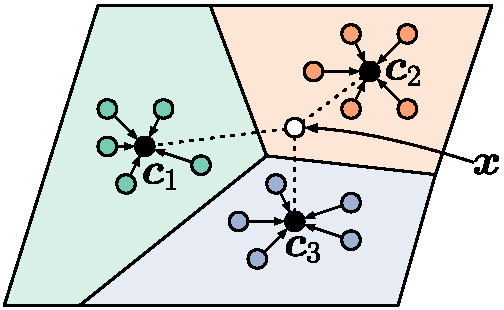
\includegraphics[scale=0.85]{chapters/assets/fsl/prototype_fewshot_v3.pdf}
    \caption{Few-shot prototypes $\symbfit{c}_k$ are computed as the mean of embedded support examples for each class. Image sourced from \parencite{Snell2017PrototypicalLearning}.}
    \label{fig:protonets}
\end{figure}

The distribution over classes for a given query input $\symbfit{x}$ is a softmax over the inverse of the distances between the embedding of the query data and the prototype vectors:
\begin{equation}
    P(y=k\vert\symbfit{x})=\operatorname{softmax}\left(-d(f_\theta(\symbfit{x}), \symbfit{c}_k)\right) = \frac{\exp(-d(f_\theta(\symbfit{x}), \symbfit{c}_k))}{\sum_{k^\prime \in \mathcal{C}}\exp(-d(f_\theta(\symbfit{x}), \symbfit{c}_{k^\prime}))}
    \label{eqn:fsl-proto-classification}
\end{equation}
where $d$ can be any distance function, as long as it is a differentiable operation to allow gradient-based learning. In the original work, \textcite{Snell2017PrototypicalLearning} use the Euclidean distance metric.

Learning is carried out by minimising the negative log likelihood $J(\symbfit{\theta})$ and performing stochastic gradient descent over the same to update the kernel's parameters $\symbfit{\theta}$:
\begin{equation}
    J(\symbfit{\theta})=-\log P_{\symbfit \theta}(y=k \vert \symbfit{x}).
\end{equation}

\subsection{Re-interpretation of the Prototypical Classifier as a Linear Model}\label{ssec:proto-reint-linmodel}

As explained by \textcite{Snell2017PrototypicalLearning}, Prototypical Networks can be re-interpreted as a linear classifier applied to a learned representation $f_{\symbfit{\theta}}(\bfitx)$. Using the Euclidean distance \(d(\symbfit{z}_i, \symbfit{z}_j)=\left\|\symbfit{z}_i-\symbfit{z}_j\right\|^{2}\) in \Cref{eqn:fsl-proto-classification} makes the model equivalent to a linear model and the output logits can be expressed as:
\begin{align}
        -\left\|f_{\symbfit \theta}(\symbfit{x})-\symbfit{c}_{k}\right\|^{2}&=-f_{\symbfit \theta}(\symbfit{x})^{\top} f_{\symbfit \theta}(\symbfit{x})+2 \symbfit{c}_{k}^{\top} f_{\symbfit \theta}(\symbfit{x})-\symbfit{c}_{k}^{\top} \symbfit{c}_{k} \nonumber\\
        2 \symbfit{c}_{k}^{\top} f_{\symbfit \theta}(\symbfit{x})-\symbfit{c}_{k}^{\top} \symbfit{c}_{k}&=\symbfit{W}_{k}^{\top} f_{\symbfit \theta}(\symbfit{x})+b_{k} \text {, where } \symbfit{W}_{k}=2 \symbfit{c}_{k} \text { and } b_{k}=-\symbfit{c}_{k}^{\top} \symbfit{c}_{k}
        \label{eqn:proto-lin-layer}
\end{align}

Based on \Cref{eqn:proto-lin-layer}, we can see that the $k\textsuperscript{th}$ unit of an equivalent linear layer therefore has weights \(\symbfit{W}_k=2\symbfit{c}_k\) and biases $b_k=-\symbfit{c}_{k}^{\top} \symbfit{c}_{k}=-\left\| \symbfit{c}_k \right\|^2$, which are both differentiable with respect to $\symbfit{\theta}$ as they are a function of $f_{\symbfit \theta}$. \textcite{Snell2017PrototypicalLearning} hypothesise that this linear classifier is effective because all the required non-linearity can be learnt within the embedding function $f_{\symbfit \theta}$.

This interpretation also allows us to create a task-specific linear classifier layer for each episode where the layer weights are initialised based on the equivalent weights and biases of the prototypical network as defined above and in \Cref{eqn:proto-lin-layer}. Subsequently, this layer can then be optimised as usual on the given support set. When computing the update for $\symbfit{\theta}$, we allow gradients to flow through the Prototypical Network-equivalent linear layer; we may also \textbf{freeze} the embedding network $f_{\symbfit \theta}$ if we only wish to train the Prototypical Network-equivalent linear layer.


\section{Unsupervised Few-Shot Learning}\label{sec:u-fsl}

So far, we have only discussed few-shot learning in a supervised setting. However, a more challenging scenario is the unsupervised setting. Recall that the dataset in the supervised setting is given as \(\mathcal{D} = \{({\symbfit x}_i, y_i)\}_{i = 1}^{M}\) which implies that we have the true class labels $y_i$ available during training time. In the unsupervised setting, we no longer have access to the true labels during the training period. 

Then a question naturally arises: How do we create valid tasks (see \Cref{sec:formalising-fsl}) if we do not have access to the true labels? This is an important question; consider \Cref{fig:fsl-tasks} where we illustrate (\nwks{3}{2}) shots, we see that each of the $3$ classes has exactly $2$ samples. Tasks like this would be difficult to create without labels. To overcome this, we shall discuss some creative methods in the following sections.

\subsection{CACTUs}\label{ssec:ufsl-cactus}
CACTUs was one of the first methods aimed at solving the unsupervised few-shot learning problem \parencite{Hsu2018UnsupervisedMeta-Learning}. CACTUs uses MAML as part of its training mechanism to obtain a generalisable model. CACTUS also retains the episodic task-based training strategy introduced by MAML \parencite{Finn2017Model-agnosticNetworks}. Unlike MAML, however, a major aspect of CACTUs is dedicated to a clever \textbf{task creation} technique, as it cannot be fed standard tasks, as discussed above.
\begin{figure}[ht]
    \centering
    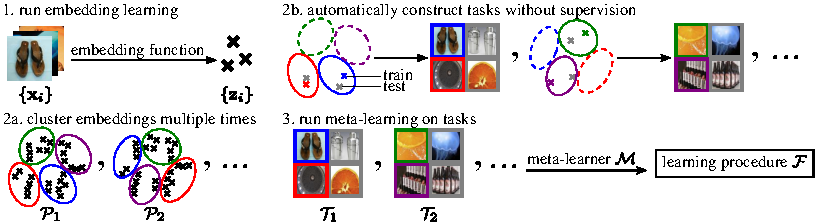
\includegraphics[width=\linewidth]{chapters/assets/fsl/cactus.pdf}
    \caption{Illustration of CACTUs. }
    \label{fig:cactus}
\end{figure}
The idea of CACTUs is to use a separate embedding learning algorithm $\mathcal{E}$ on $\bfitx_i \in \mathcal{D}$ to produce embeddings $\{\symbfit{z}_i\}$. It then uses $k$-means clustering on $\{\symbfit{z}_i\}$ $P$ times to generate a set of partitions $\mathcal{P}_P = \{\mathcal{C}_P\}$. CACTUs can technically make use of any self-supervised (more generally, unsupervised) representation learning methods to train $\mathcal{E}$. \textcite{Hsu2018UnsupervisedMeta-Learning} choose to use DeepCluster \parencite{caron2018deep}, BiGAN \parencite{berthelot2018understanding}, ACAI \parencite{donahue2016adversarial}, and InfoGAN \parencite{chen2016infogan}. 

CACTUs then samples a partition $\mathcal{P}$ randomly from the set of parititons $\{\mathcal{P}_P\}$, following which a cluster $\mathcal{C}_n$ is randomly sampled from the partition $\mathcal{P}$. The cluster sampling process is carried out $N$ times for each of the classes desired in a (\nwks{N}{K}) task. Similarly, the process is repeated for $Q$ query images. Finally, the randomly sampled support and query images are used to create a \textbf{synthetic} task that is fed into MAML.

A major concern here is that CACTUs is dependent on bigger models, like AlexNet \parencite{AlexNet2012}, using powerful self-supervised learning methods on a small dataset like \miniImagenet{}. The embeddings (representations) generated by this larger model are then used to create synthetic tasks to train a simpler Conv$4$ architecture. It has been known for quite some time that larger models consistently offer better performance and representations \parencite{Dosovitskiy2020, He2015}, these better representations indirectly aid a smaller Conv$4$ to learn better. Therefore, defeating the purpose of a self-contained end-to-end few-shot learning algorithm by using parameter heavy models and computationally intensive algorithms.

\subsection{UMTRA} \label{ssec:umtra}

Unsupervised Meta-learning with Tasks constructed by Random sampling and Augmentation (UMTRA), is another method that uses a MAML style training strategy with inner and outer objectives in an unsupervised fashion.
Unlike CACTUs (\Cref{ssec:ufsl-cactus}), the focus of UMTRA is not on generating ideal tasks. 
Instead, the idea behind UMTRA can be summarised in one line; it is an unsupervised method that uses augmentations of the images in a given episode to create a valid query set. This allows it to generate a \textquote{labelled} query set for the outer objective and can perform well if we span the entire space of the classes.

\begin{figure}[ht]
    \centering
    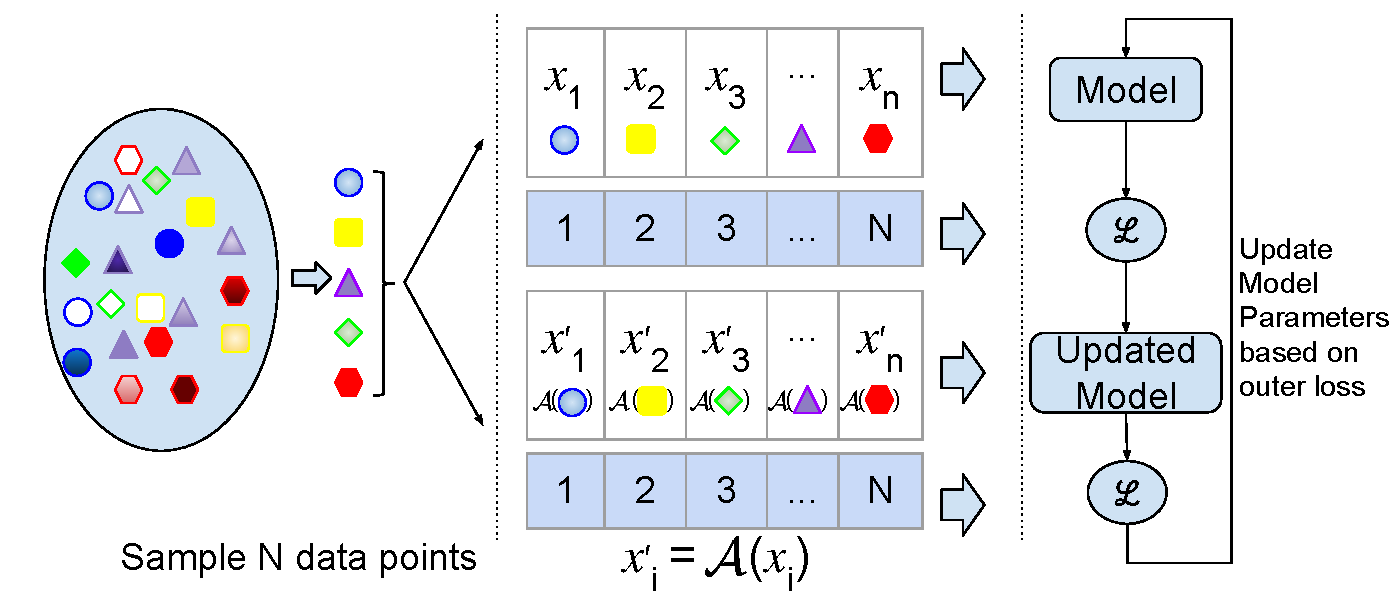
\includegraphics[width=\linewidth]{chapters/assets/fsl/UnsupervisedMetaTraining3.pdf}
    \caption{We start from a dataset of unlabelled data. The training data is created by randomly choosing $N$ samples $\bfitx_i$ from the dataset. The query data is created by applying the augmentation function $\mathcal{A}$ to each sample from the training data. Image borrowed from \parencite{Khodadadeh2018UnsupervisedClassification}.}
    \label{fig:umtra}
\end{figure}

The functioning of UMTRA is illustrated in \Cref{fig:umtra}, where $N$ data points are randomly sampled, each of the $N$ random samples is given its own unique class label. Subsequently, each sample $\symbfit{x}_i$ is augmented using an augmentation function $\mathcal{A}$ that gives an augmented image $\symbfit{x}_i^\prime$. 
The reason this works is that each augmented image will share its class label with the original image. Therefore, we can be sure that the outer objective will always have samples of the same class available for it to learn from. 

\subsection{ProtoTransfer}\label{ssec:prototransfer}

Until now, we have discussed \nameref{ssec:ufsl-cactus} and \nameref{ssec:umtra}, both of which use \nameref{sec:maml} and episodic training to solve the few-shot classification problem.
However, several recent studies have questioned the necessity of meta-learning for few-shot classification \parencite{goodemballneed2020, Medina2020Self-SupervisedClassification, dhillon2019baseline, ziko2020laplacian, boudiaf2020information,chen2021self}.
They report competitive performance on few-shot benchmarks without episodic training or few-shot task-based experiences during training. These methods follow the an approach where they aim to solve the few-shot learning problem by fine-tuning a pre-trained feature extractor with a standard cross-entropy loss. In fact, both our methods \ccclr{} and \samptr{} comfortably outperform unsupervised and supervised MAML based methods.

Some of these methods \parencite{Medina2020Self-SupervisedClassification, goodemballneed2020, das2022confess} in the space demonstrate that the transfer learning approach outperforms meta-learning based methods in standard in-domain and cross-domain settings, where the training and novel classes come from totally different distributions.
%
\begin{figure}[ht]
\centering
\begin{minipage}{\textwidth}
  \centering
  \setlength{\unitlength}{1cm}
  
    \begin{picture}(13.5,5)
    \put(0,0){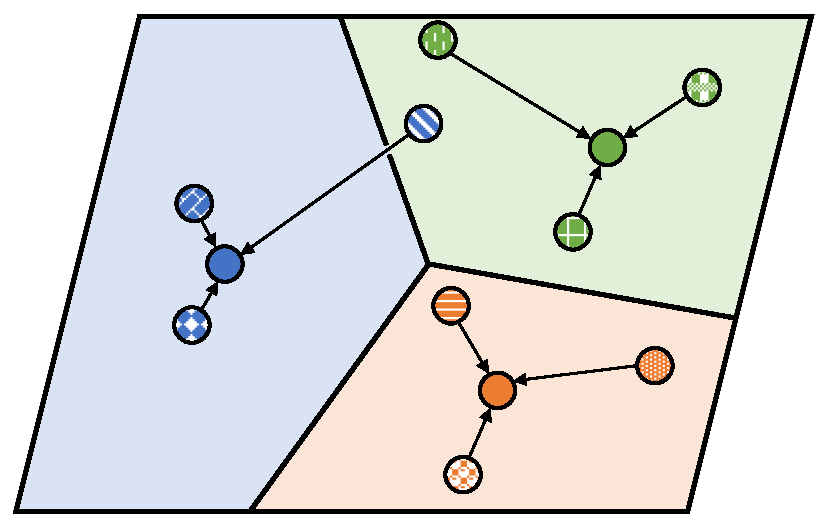
\includegraphics[scale=0.45]{chapters/assets/fsl/selfsupproto.pdf}}
    
    \put(7.3,0){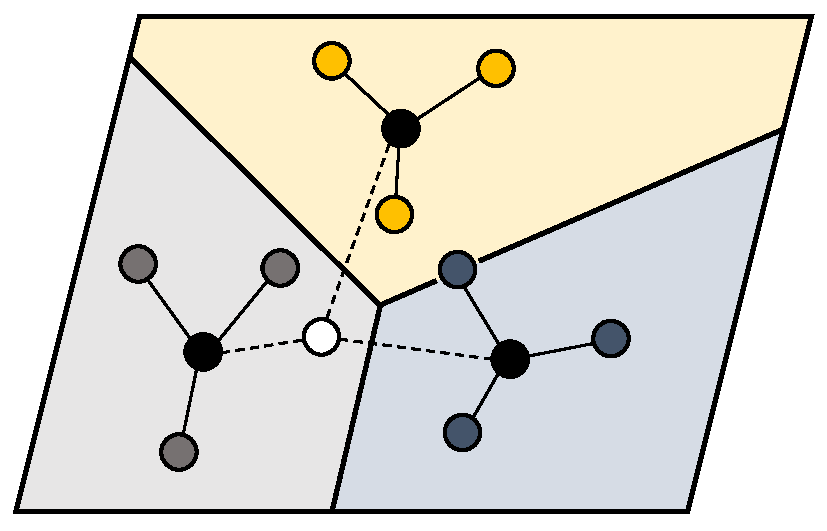
\includegraphics[scale=0.45]{chapters/assets/fsl/protofinetune.pdf}}
    \put(1.9,1.9){$\scriptstyle f_\theta(\symbfit{x}_i)$}
    \put(1,1.2){$\scriptstyle f_\theta(\tilde{\symbfit{x}}_{i,1})$}
    \put(1,2.8){$\scriptstyle f_\theta(\tilde{\symbfit{x}}_{i,2})$}
    \put(3.1,2.7){$\scriptstyle f_\theta(\tilde{\symbfit{x}}_{i,3})$}
    
    \put(4.8,2.8){$\scriptstyle f_\theta(\symbfit{x}_{2})$}
    
    \put(3.9,.8){$\scriptstyle f_\theta(\symbfit{x}_{1})$}

    \put(10.5,2.9){$\scriptstyle \symbfit{c}_{1}$}
    \put(8.4,1.1){$\scriptstyle \symbfit{c}_{2}$}
    \put(11.3,1.1){$\scriptstyle \symbfit{c}_{3}$}
    
    \put(9.3,1.1){$\scriptstyle f_\theta(\symbfit{q})$}
    \end{picture}\\
    \hspace{-.2cm}(a) Self-Supervised Prototypical Pre-Training \hspace{.8cm} (b) Prototypical Fine-Tuning \& Inference
  
  \label{fig:sub2}
\end{minipage}
\caption{Self-Supervised Prototypical Transfer Learning. (a): In the embedding, original images $\symbfit{x}_i$ serve as class prototypes around which their $Q$ augmented views $\tilde{\symbfit{x}}_{i,q}$ should cluster. (b): Prototypes $\symbfit{c}_{k}$ are the means of embedded support examples for each class $n$ and initialise a final linear layer for fine-tuning.
An embedded query point $\symbfit{q}$ is classified via a softmax over the fine-tuned linear layer.
Image sourced from \parencite{Snell2017PrototypicalLearning}.}
\label{fig:prototransfer}
\end{figure}

One such method that we shall focus on is ProtoTransfer \parencite{Medina2020Self-SupervisedClassification}. Unlike \nameref{ssec:ufsl-cactus} and \nameref{ssec:umtra} ProtoTransfer does not rely on a task-based episodic training regime and does not use MAML for its training. 
Instead, ProtoTransfer uses a form of \nameref{sec:contrastive-learning} that is similar to and inspired by \nameref{ssec:simclr}. 
ProtoTransfer consists of two phases: (i) \textbf{pre-training} on a large dataset of \textquote{base} classes. This is followed by (ii) \textbf{fine-tuning} on an unseen dataset consisting of \textquote{novel} classes. 

\textcite{Medina2020Self-SupervisedClassification} call their pre-training method \textbf{ProtoCLR}, and in principle it is extremely similar to \nameref{ssec:simclr}.
ProtoCLR uses the original image, $\bfitx_i$, and $Q$ augmentations, $\{\Tilde{\bfitx}_{i,q}\}_{q=1}^Q$. In order to learn the metric embedding function, $f_{\symbfit{\theta}}(\cdot)$, a contrastive loss is used here to ensure that all $Q$ augmentations have the same representation as the original image. 
\nameref{ssec:simclr} on the other hand, uses two augmentations of the same image and ensures similarity between them by means of a contrastive loss. Although not the same, one can see that ProtoCLR is very inspired by methods such as \nameref{ssec:simclr}.

\begin{tcolorbox}[title=Link between self-supervision and an episode]
Consider a mini-batch that contains $n$ random samples $\{{\bfitx_i}\}_{i=1 \ldots n}$ from the training set $\mathcal{D}^\textup{tr}$.
As our self-supervised setting does not assume any knowledge about the base class labels $\symbfit{y} \in \mathcal{D}^\textup{tr}$, we treat each sample as its own class. Thus, each sample $\bfitx_i$ serves as a $1$-shot support sample and class prototype. For every prototype $\bfitx_i$, $Q$ randomly augmented samples $\Tilde{\bfitx}_{i,q}$ are used as query samples.
\end{tcolorbox}

Following the ProtoCLR pretraining phase, we have a fine-tuning phase called \textbf{ProtoTune} and it is a supervised phase. In the fine-tuning phase, the learnt embedding $f_{\symbfit{\theta}}(\cdot)$ is used to address the \textbf{target problem} of few-shot image classification, where we are presented with test tasks episodically, each with their own support and query.
ProtoTune is based on the linear layer interpretation of the Prototypical classifier (see \Cref{ssec:proto-reint-linmodel}). It uses each task's support set to initialise the linear classifier and fine-tune it on subsets of the support set for some iterations, randomly sampling different subsets of support images in each iteration.

ProtoTransfer was chosen as the base for \ccclr{} and \samptr{} due to its robustness and simplicity of self-supervision. Although both \ccclr{} and \samptr{} are inspired by ProtoTransfer, the similarities only extend to their shared self-supervised nature and in the case of \samptr{} there is a reimagined network and fine-tuning phase based on \nameref{chap:optimal-transport} that has the potential to be useful even outside of few-shot learning.

\newcommand{\mcX}{\mathcal{X}}
\newcommand{\bfitr}{\symbfit{r}}
\newcommand{\bfitc}{\symbfit{c}}

\chapter{Optimal Transport}\label{chap:optimal-transport}

In most decisions pertaining to life and sciences, the \textquote{shortest path} approach acts as the guiding strategy. Whenever a commodity, a person, a single bit of information, or any entity that is available at a given point and needs to be sent to a target point, one should ideally favour a way that uses the least effort possible. Typically, one would achieve this by moving an entity along a straight line from point A to point B on a plane.
The theory of \textbf{optimal transport} (OT) generalises that intuition in the case where, instead of moving only item at a time, we are concerned with the problem of simultaneously moving several items (or a continuous distribution) from configuration onto another.

As vacation planners can attest to, planning the transportation for a group of individuals involved in the event, with the added constraint that they reach a given target configuration upon arrival, is considerably more tortuous than carrying it out for a single individual. In fact, thinking in terms of groups or rather distributions requires more advanced mathematical thinking and formalism, which was first explored by \textcite{monge1781memoire}. Regardless of how complicated this formalism might be, it has deep rooted connections to our daily life. 
Transportation, be it of people, commodities, or information, rarely involves moving items. All major problems in economics, such a supply chain logistics, production planning, or warehousing involve moving distributions, and that motif consistently appears in  

\section{A brief historical context of Optimal Transport}\label{sec:ot-history}

The inception of optimal transport began in the late $18\textsuperscript{th}$ century under the rule of Louis \RN{16}, around $1781$, almost a decade before the French revolution of $1789$. The French physicist and mathematician Gaspard Monge\footnote{\url{https://mathshistory.st-andrews.ac.uk/Biographies/Monge/}} was the first to formulate the mathematical problem of \textquote{Excavation and embankments} (\citetitle{monge1781memoire}) - how to transport soil during the construction of forts and roads with minimal transport expenses. But what does shoveling dirt have to do with AI, statistics, or machine learning? Interestingly, the framework devised by \citeauthor{monge1781memoire} provides a formulation for comparing probability distributions.
Let us think of probability density functions as piles of dirt, where the \textquote{height} of the pile corresponds to the probability density at that point, and shoveling dirt between the piles as moving probability from one point to another, at a cost proportional to the distance between these two points.

\begin{figure}[ht]
    \centering
    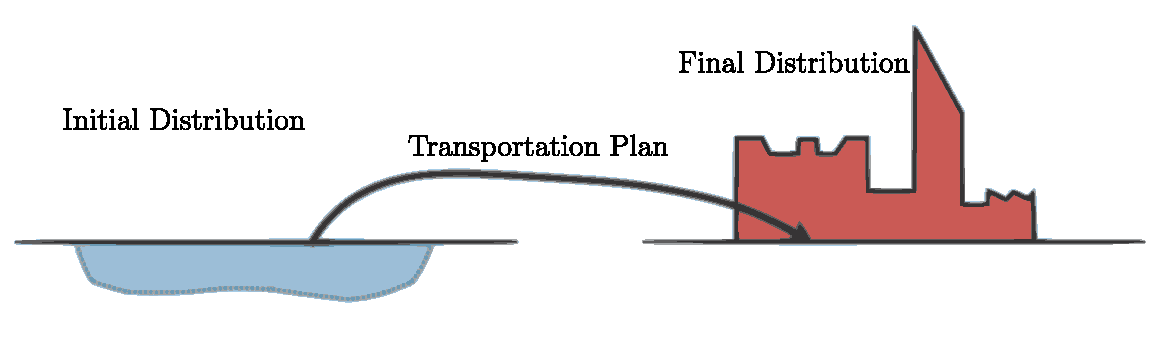
\includegraphics[width=\linewidth]{chapters/assets/ot/monge.pdf}
    \caption{Monge's problem of moving soil.}
    \label{fig:monges-problem}
\end{figure}

This modern form of optimal transport and the one that is in use today in various applications was first formulated by the nobel laureate Leonid Vitaliyevich Kantorovich\footnote{\url{https://www.nobelprize.org/prizes/economic-sciences/1975/kantorovich/biographical/}}, the father of linear programming. 
It was his work in \citeyear{Kantorovich42} which cast the transportation as a probablistic measure on a metric space $\mcX$, where in a measure $\alpha$ is the intial one that needs to be transported to the second and final measure $\beta$, that is, the desired distribution after transportation. A transportation plan, as it is called by \citeauthor{Kantorovich42}, is also some probability measure $\pi$ on the Cartesian product of the space with itself $\mcX \times \mcX$.
We shall go into a bit more depth in later sections of this chapter.

It would be several years later that this theory was rediscovered thanks to the work of \textcite{Brenier1991PolarFunctions} and others that this theory provided a crucial basis for research, with strong links to convexity, partial differential equations, and statistics. Today, researchers in computer science disciplines, imaging, and more generally data scientists recognise that optimal transport theory grants powerful tools to study distributions in an abstract context, such as comparing readily available distributions.

\section{Discrete Optimal Transport}\label{sec:discrete-ot}

Since our work mostly deals with atomic items, we choose to focus on the discrete formulation instead of the continuous formulation, although it must be noted that concepts spoken about here do not change drastically in the continuous domain.

\subsection{Asssignment Problem}\label{ssec:ot-assignment-prob}

In its most basic form, OT can be viewed as an assignment problem between sets of entities, that is, among all possible configurations, which one is the best? This question is quite restrictive in the sense that we can only work with two sets of the same total size, that is, an \textit{initial} set and a \textit{target} set.

Each set can be represented as a histogram (or vector) $\bfitr$, that belongs to the probability simplex - the components of the vector sum up to $1$:
\begin{equation}
    \bfitr \in \left\{ x = (x_1, …, x_N) \in \mathbb{R}^N : \sum_{i=1}^N x_i = 1 \right\} 
    \label{eqn:r-simplex-defn}
\end{equation}

If we consider $\symbf{C}_{i,j}$ as the cost of moving an element from $i$ to $j$, then the quantity we wish to minimise is $\sum_{i} \symbf{C}_{i,\sigma(i)}$ , where $\sigma$ is a \textbf{permutation} of the set $\{1,\ldots, N\}$. This permutation represents an assignment of the bin $i$ of the first histogram to the output positions $j$ in the second histogram.

In this form optimal transport is fundamentally a combinatorial problem, and may be summarised as: 
How can we assign every element $i \in \{1, \ldots, N\}$ to elements $j \in \{1, \ldots, N\}$ in order to minimise $\sum_{i} \symbf{C}_{i,\sigma(i)}$.

The result of this search is called \textbf{optimal assignment}. As you may have guessed already, there can be $N!$ possible solutions to this problem; therefore, as $N$ grows this problem quickly becomes intractable.

\begin{figure}
    \centering
    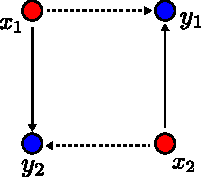
\includegraphics{chapters/assets/ot/monge1.pdf}
    \caption{Non-unique assignments. The other solution is dashed.}
    \label{fig:ot-non-uniq}
\end{figure}

An important aspect is that this assignment is not unique. \Cref{fig:ot-non-uniq} is an example where two elements are assigned to two other elements that together form the four corners of a square.

\subsection{Working with asymmetric histograms (distributions)}\label{ssec:ot-assym}

Requiring two equally sized histograms is a very strong constraint, hardly any real-world problems present themselves in this manner. By expanding the previous problem definition to a broader class of histograms, we obtain the Monge problem. In this version of the problem, several points $\bfitx_i$ can map to the same $y_j$ and their weights will be summed.

\begin{figure}[ht]
    \centering
    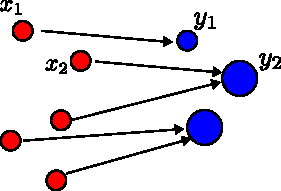
\includegraphics{chapters/assets/ot/monge2.pdf}
    \caption{The Monge problem.}
    \label{fig:ot-assym}
\end{figure}

In this case, the mapping between inputs and outputs is no longer a combinatorial permutation, but a \textbf{surjective} map $\pi$. If points $\{\bfitx_1, \ldots, \bfitx_n\}$ have weights $\bfitr=\left(r_1, \ldots, r_n\right)$ and points $\left\{y_1, \ldots, y_m\right\}$ have weights $\bfitc=\left(c_1, \ldots, c_m\right)$, $\pi$ must verify:
\begin{equation}
    \forall j \in\{1, \ldots m\}, \quad c_{j}=\sum_{i: \pi\left(x_{i}\right)=y_{j}} a_{i}
    \label{eqn:ot-mass-conserv}
\end{equation}

\begin{tcolorbox}[title=Surjective functions]
A surjective function is a function $f$ that maps an element $\bfitx$ to every element $y$; that is, for every $y$, there is an $\bfitx$ such that $f(\bfitx) = y$. In other words, every element of the function's codomain is the image of at least one element of its domain. It is not required that $\bfitx$ be unique; the function $f$ may map one or more elements of $X$ to the same element of $Y$. 
\end{tcolorbox}

Even with this formulation, it does not make our job easier, the mass conservation constraint stated in \Cref{eqn:ot-mass-conserv} must be satisfied, while our problem still continues to remain an assignment problem. We are still assigning element $\bfitx_i$ to element $\symbfit{y}_j$.

\subsection{The Kantorovich relaxation}\label{ssec:ot-kantorovich-relax}

Even with the above extension, this formulation of the optimal transport problem is still too constrained to be practically useful in many cases. As alluded to earlier in \Cref{sec:ot-history}, in 1942 \citeauthor{Kantorovich42} was instrumental in making OT viable for practical use. Kantorovich introduced a key idea, which is to \textbf{relax} the deterministic portion of the transportation. Points in the source histogram (or domains or distributions), $\bfitx_i$, no longer have to map to a single target point and can be \textit{fragmented} into \textit{partial} assignments, this is called \textbf{mass splitting}.

\begin{tcolorbox}[title=Relaxation]
Relaxation refers to the modelling strategy in mathematical optimisation and associated fields. Relaxation stands to be the approximation in relation to the difficult problem with regard to a nearby problem which stands to be easy to compute/solve.
\end{tcolorbox}

This new relaxed formulation was much more suitable for real-world situations, such as logistical problems. \textcite{hitchcock1941distribution} stated a version of this problem as follows:
When several factories supply a product to a number of cities, we desire the least costly manner of distribution. Due to freight rates and other expenses, the cost of a ton of product to a particular city will vary according to which factory supplies it and will also vary from city to city.
\begin{figure}[ht]
    \centering
    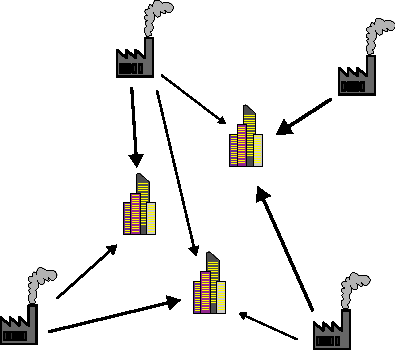
\includegraphics{chapters/assets/ot/logistic.pdf}
    \caption{Factories with different supply capacities have to deliver goods to cities with various demands.}
    \label{fig:ot-factories}
\end{figure}

To reflect this change, we will slightly modify our previous formulation by replacing the permutation function $\sigma$ by a coupling matrix $\symbf{\pi} = \symbf{\pi}_{i j} \in \mathbb{R}_{+}^{n \times m}$. In \Cref{fig:ot-factories}, each $\symbf{\pi}_{i j}$ would be the weight of the arrow from factory $i$ to city $j$.
As stated we have earlier $\bfitr$ is a probability simplex, the same is applicable to $\bfitc$. With this established, all possible assignments can be written as:
\begin{equation} 
\label{eqn:ot-def}
\symbf{\Pi}(r, c)=\left\{\pi \in \mathbb{R}_{+}^{n \times m} \mid \pi \symbf{1}_{m}=r, \pi^{\top} \symbf{1}_{n}=c\right\}.
\end{equation}

$\symbf{\Pi}(r, c)$ contains all non-negative $n \times m$ matrices for which all rows sum up to $\bfitr$ and all columns sum up to $\bfitc$. 
This makes $\symbf{\Pi}(r, c)$ a \textbf{polytope} of $\bfitr$ and $\bfitc$, representing a polyhedral set of $n \times m$ matrices.
$\symbf{\Pi}(r, c)$ is then essentially a collection of \textbf{transport plans} (coupling matrix) of which some are better than others.
Bear in mind that both $\bfitr$ and $\bfitc$ can only be accessed through a finite set of samples, each, in \Cref{fig:ot-factories} that means a limited set of factories and cities.

\begin{tcolorbox}[title=Polytope]
The word polytope is used to mean a number of related, but slightly different, mathematical objects. A convex polytope may be defined as the convex hull of a finite set of points that are always bounded. \textquote{Convex} implying that there is a minimum point.
\end{tcolorbox}

\textcite{cuturi2013sinkhorn} also gives a probabilistic interpretation for $\symbf{\Pi}(r, c)$: for $A$ and $B$ two multinomial random variables taking values in  $\{\bfitx_1, \ldots, \bfitx_n\}$ and  $\{\symbfit{y}_1, \ldots, \symbfit{y}_m\}$ each with distribution $r$ and $c$ respectively, the set $\symbf{\Pi}(r, c)$ contains all possible \textit{joint probabilities} of $(A, B)$. Any matrix $\pi \in \symbf{\Pi}(r, c)$ can be identified with a joint probability for $(A, B)$ such that $p(A = i, B = j) = p_{ij}$.

Given a cost matrix $\symbf{C}$, the cost of mapping $r$ to $c$ using a transport plan (or joint probability) $\pi$ can be quantified as $\langle \pi, C \rangle_{F}$, we can now formulate the problem in a much cleaner fashion:
\begin{equation}
    \pi^\star = \min_{\pi \in \symbf{\Pi}(r, c)} \sum_{i,j} \symbf{C}_{i,j}{\pi}_{i,j} = \min_{\pi \in \symbf{\Pi}(r, c)} \langle \symbf{\pi}, \symbf{C} \rangle_{F}
    \label{eqn:ot-objective-relaxed}
\end{equation}
where $\pi^\star$ is the optimal transport plan and $\langle \cdot, \cdot \rangle_{F}$ is the Frobenius dot product. When the cost matrix is based on a valid distance metric, the optimum $\pi^\star$ is known as \textbf{Wasserstein distance}. It is basically a distance between two probability distributions. It is sometimes also called \textbf{earth mover distance} as it can be interpreted as how much \textquote{dirt} you have to move to change one \textquote{landscape} (distribution) in another.

\subsection{Entropic Regularisation}\label{ssec:ot-entropic-reg}

Regularising the optimal transport problem was originally proposed by \textcite{hitchcock1941distribution}. It is a method for \textbf{approximating} solutions to the optimal transport problem by adding a regularising term to the objective function in \Cref{eqn:ot-objective-relaxed}.

We start by defining the entropy of the coupling matrix, $\pi$:
\begin{equation}
    H(\symbf{\pi}) = -\sum_{ij}\symbf{\pi}_{ij}\log\symbf{\pi}_{ij}.
\end{equation}
In information theory, the entropy of a random variable is the average level of \textquote{information}, \textquote{surprise}, or \textquote{uncertainty} inherent to the variable's possible outcomes. Based on this understanding, a matrix with low entropy will be sparser, with most of its non-zero values concentrated in a few points. Conversely, a matrix with high-entropy will be \textit{smoother}, with the maximum entropy achieved with a uniform distribution of values across its elements. With a regularisation coefficient $\varepsilon$, we can include this in the optimal transport problem to encourage smoother coupling matrices:
\begin{align}
& \symbf{\pi}^\star = \min_{\pi \in \symbf{\Pi}(r, c)}\langle\symbf{\pi},\symbf{C}\rangle_{F} -\varepsilon H(\symbf{\pi})\\
\text{subject to } &\symbf{\pi}\symbf{1} = \bfitr \nonumber\\
&\symbf{\pi}^{\top}\symbf{1} = \bfitc. \nonumber
\end{align}

By increasing the value of $\varepsilon$, the resulting coupling matrix will be smoother, and as $\varepsilon \rightarrow 0$ the coupling matrix will be sparser (or sharper) and the solution will be closer to that of the original relaxed OT problem in \Cref{eqn:ot-objective-relaxed}. The intuition behind entropy regularisation is similar to the temperature-normalised cross-entropy (NT-Xent) discussed in \Cref{ssec:simclr}.

The addition of this entropic regularisation makes this optimisation problem convex. Therefore, there is a unique optimal solution $\symbf{\pi}^\star$. It can be shown that the solution to this regularised problem has the following form:
\begin{equation}
    \forall (i,j) \in \{1,…,n\}\times \{1, …, m\},\quad \symbf{\pi}_{i,j} = \symbf{u}_i \symbf{K}_{i,j} \symbf{v}_j, \quad \symbf{\pi} = \operatorname{diag}(\symbf{u}) \symbf{K} \operatorname{diag}(\symbf{v})
    \label{eqn:ot-mat-scaling}
\end{equation}
where $\symbf{K}$ is a kernel matrix $\symbf{K}_{i,j}=\exp{(-\sfrac{\symbf{C}_{i,j}}{\varepsilon})}$ calculated with $\symbf{C}$ and $\symbf{u}$ and $\symbf{v}$ are unknown scaling variables. This formulation is important because we now have an explicit formula for an optimal coupling matrix.

\subsection{Sinkhorn-Knopp Algorithm}\label{ssec:ot-sk}
The problem in \Cref{eqn:ot-mat-scaling} is known as the matrix scaling problem, we are trying to find two scaling vectors, $\symbf{u}$ and $\symbf{v}$, that when multiplied with $\symbf{K}$ give $\symbf{\pi}$. We can find these vectors by alternatively updating $\symbf{u}$ and $\symbf{v}$ using \textbf{Sinkhorn's algorithm}:
\begin{align}
\symbf{u}^{(k+1)} &= \frac{\symbfit{r}}{\symbf{K}\symbf{v}^{(k)}}\\
\symbf{v}^{(k+1)} &= \frac{\symbfit{c}}{\symbf{K}^{\top}\symbf{u}^{(k+1)}}
\end{align}

The convergence proof of this algorithm is attributed to \textcite{Sinkhorn1967}. The algorithm not only converges, but does so at a linear rate. Since these iterations are solving a regularised version of the original problem, the corresponding Wasserstein distance that results is sometimes called the Sinkhorn distance. Since these iterations form a sequence of linear operations, it is straightforward for deep learning models to backpropagate through these iterations; in other words, the Sinkhorn-Knopp algorithm is differentiable.

Following a paper from \textcite{cuturi2013sinkhorn} called \citetitle{cuturi2013sinkhorn} that showed Sinkhorn updates were effieicnt and scalable approximation to OT, there has been a renewed interest in the community.
Several performant ideas in the self-supervised learning space such as SWaV \parencite{caron2020unsupervised} and SeLa \parencite{asano2019self} have made use of the Sinkhorn-Knopp algorithm in their methods. Furthermore, the supervised few-shot learning space has also seen the usage of Sinkhorn-Knopp in methods like PT-MAP \parencite{hu2021leveraging} which use the algorithm to assign labels to unlabelled query samples.


% \section{A sweet example}\label{sec:ot-example}
% % TODO: michiel stock's post example here
% Consider an example where we have collection of sweets that must be given to a set of people based on their preferences. This is an assignment problem. 
% \begin{figure}[ht]
%     \centering
%     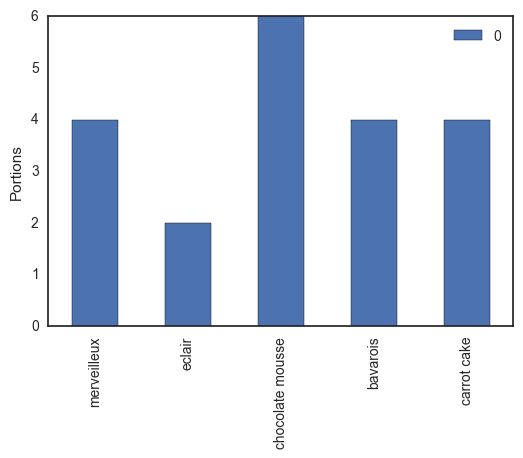
\includegraphics[scale=0.4]{chapters/assets/ot/desserts.png}
%     \caption{A distribution (histogram) of various sweets. If we mentally cut all these sweets into portions, we have twenty shares.}
%     \label{fig:ot-desserts}
% \end{figure}

\chapter{\ccclr{}: Additional Materials}\label{sec:ccclr-additional-mat}

This chapter deals with the justification of certain design choices made for \ccclr{} (\Cref{chap:c3lr-art}), that could not be covered in the original article due to space constraints.
The algorithm from the article is made available below for convenience.
\begin{algorithm}[ht]
    \caption{\scalebox{.9}{Class-Cognizant Contrastive Learning (\ccclr{})}}\label{alg:pclr-c}
    
    % \setstretch{.8}
    \SetAlgoSkip{}
    \SetKwInOut{Input}{input}
    \SetKwInOut{Output}{output}
    \SetKwInput{Require}{Require}
	\SetKwInput{Return}{Return}
	\SetKw{Let}{let}
	\SetKwRepeat{Do}{do}{while}
	
	\SetAlgoLined
	\LinesNumbered
	\DontPrintSemicolon
	\SetNoFillComment
    \Require{$L$, $Q$, $f_\phi$, $\mathcal{A}$, $\alpha$, $d[\cdot, \cdot]$}

    \While {not done}{
        Sample minibatch $\left\{\symbfit{x}_{i}\right\}_{i=1}^{L}$\;
        \ForAll{$i \in\{1, \ldots, L\}$} {
            \ForAll{$q \in\{1, \ldots, Q\}$}{
                $\tilde{\symbfit{x}}_{i, q}=\psi^{q}(\symbfit{x}_{i})$; $\psi^{q} \sim \mathcal{A}$.\;  
            }
        }
        $\symbf{R} = \texttt{ReRank}$\scalebox{.8}{$\left(\left[ f_{\phi }\left(\{\symbfit{x}_{i}\}_{i=1}^{L}\right) ,f_{\phi }\left(\left\{\tilde{\symbfit{x}}_{i,\ q}\right\}_{i=1,q=1}^{L,Q}\right)\right]\right)$}\; 
        
        
        $\mathcal{C} = \{\symbfit{C}_1 ,\symbfit{C}_2 ,\dotsc ,\symbfit{C}_{P}\} \gets \texttt{HDBSCAN}(\symbf{R})$\;
        
        
        $\mathcal{M} = \{{\symbf m}_{p}\}_{p = 1}^P;$ \hspace{0.1cm} ${\symbf m}_p = \frac{\sum _{x_{j} \in \symbfit{C}_{p}} x_{j}}{|\symbfit{C}_{p} |}$\;
        
        \vspace{0.15cm}
        \Let{\scalebox{.95}{$\mathscr{r} (i,q,p)=-\log\frac{\exp\left( -d\left[ f_\phi\left(\tilde{{\symbfit x}}_{i,q}\right) ,\symbf{m}_{p}\right]\right) }{\sum_{p=1}^{P}\exp\left( -d\left[ f_\phi\left(\tilde{\symbfit{x}}_{i,q}\right) ,\symbf{m}_{p}\right]\right)}$}}\;
        \vspace{+0.15cm}
        \Let{\scalebox{.95}{$\ell(i, q)=-\log \frac{\exp \left(-d\left[f_\phi\left(\tilde{{\symbfit x}}_{i, q}\right), f_\phi\left(\symbfit{x}_{i}\right)\right]\right)}{\sum_{k=1}^{L} \exp \left(-d\left[f_\phi\left(\tilde{{\symbfit x}}_{i, q}\right), f_\phi\left(\symbfit{x}_{k}\right)\right]\right)}$}}\;
        
        \vspace{+0.15cm}
        $\mathcal{L}_{1}=\frac{1}{L Q} \sum_{p=1}^{P} \sum_{i=1}^{L} \sum_{q=1}^{Q} \mathscr{r}(i, q, p)$\;
        $\mathcal{L}_{2}=\frac{1}{L Q} \sum_{i=1}^{L} \sum_{q=1}^{Q} \ell(i, q)$\;
        
        $\mathcal{L} = \mathcal{L}_{1} + \mathcal{L}_{2}$
        
        $\phi \gets \phi-\alpha \nabla_{\phi} \mathcal{L}$\;
    }
\end{algorithm}


\section{Choice of Clustering Algorithm}\label{sec:c3lr-clustering-algo}

As we can see from \Cref{alg:pclr-c} and \cref{chap:c3lr-art}, the re-ranking step and clustering are crucial to its functioning. The purpose of this section is to show why \texttt{HDBSCAN} \parencite{McInnes2017Hdbscan:Clustering} was chosen in combination with the $k$-reciprocal Jaccardian distance \parencite{ZhongRe-rankingEncoding}. To motivate our choices we shall refer to \cref{tab:c3lr-combos}.

\begin{table}[!ht]
    \centering
    {\tabcolsep=0pt\def\arraystretch{1.1}
    \begin{tabularx}{\textwidth}{l >{\centering\arraybackslash}p{90pt} *4{@{}Y} >{\centering\arraybackslash}p{80pt}}
    \toprule
        \textbf{Method} & Clustering Algorithm  & UMAP & UMAP $\mathbb{R}^{\symbf \cdot}$ & $L$ & $B$ & Avg Test Acc ($\%$)\\ 
        \midrule
        ProtoCLR & None & \xmark & -  & 50 & 200 & 60.66 \\
        ProtoCLR & None & \xmark & - & 200 & 800 & 62.32 \\
        % \ccclr{}         & None & Pairwise & \xmark & - & 50 & 200 & 58.42 \\ 
        % \ccclr{}         & None & Pairwise & \xmark & - & 50 & 200 & 46.06 \\
        % \ccclr{}         & None & Pairwise & \xmark & - & 50 & 400 & 57.22 \\
        % \ccclr{}         & None & Centroid & No & - & 10 & 5 & 50 & 200 & 54.05 \\ 
        % \ccclr{}         & None & Centroid & No & - & 10 & 10 & 100 & 400 & 63.24 \\
        % \ccclr{}         & None & Centroid & No & - & 20 & 5 & 100 & 400 & 58.36 \\ 
        % \ccclr{}         & None & Centroid & No & - & 5 & 20 & 100 & 400 & 60.73 \\ 
        % \ccclr{}         & None & Centroid & No & - & 10 & 20 & 200 & 800 & 65.34 \\ 
        \ccclr{} (Oracle)        & None & \xmark & - & 200 & 800 & \textbf{66.86} \\ 
        \ccclr{}         & $K$-means ($K=5$)    & \cmark & 3 & 200 & 800 & 62.14 \\ 
        \ccclr{}         & $K$-means ($K=5$)    & \xmark & -  & 200 & 800 & 62.19 \\
        \ccclr{}         & $K$-means ($K=10$)   & \xmark & -  & 200 & 800 & 61.69 \\
        \ccclr{}         & $K$-means ($K=25$)   & \cmark & 3 & 200 & 800 & 62.68 \\
        \ccclr{}         & $K$-means ($K=25$)   & \xmark & -  & 200 & 800 & 63.60 \\ 
        \ccclr{}         & HDBSCAN          & \cmark & 3  & 200 & 800 & 62.46 \\
        \ccclr{}         & HDBSCAN          & \xmark & -  & 200 & 800 & 62.44 \\
        \ccclr{}         & HDBSCAN + $k$-rJd & \cmark & 2  & 200 & 800 & 63.79 \\
        \ccclr{}         & HDBSCAN + $k$-rJd & \xmark & - & 200 & 800 & \underline{64.81} \\
        \bottomrule
    \end{tabularx}}
    \caption{Table comparing design choices for \ccclr{} though accuracy ($\%$) on (\nwks{5}{5}) classification tasks. Style: \textbf{best} and \underline{second best}.}
    \label{tab:c3lr-combos}
\end{table}

\cref{tab:c3lr-combos} shows the performance of \ccclr{} with $K$-means and \texttt{HDBSCAN} as clustering algorithms of choice. The best performing variant of \ccclr{} is the \textbf{oracle} variant, this variant of the model provided access to the true labels of the data. The true labels allowed the creation of the ideal cluster centres. To understand why this is, we shall elaborate on lines $9$ and $10$ in \cref{alg:pclr-c}. In line $9$, \texttt{HDBSCAN} processes the input data and groups them, when we say that an element belongs to cluster $\symbf{C}_p$ it also implies that $\symbf{C}_p$ functions as a predicted label for that element. 
Instead of using predicted labels, the oracle variant uses actual labels. Since we know the actual grouping of elements, we can calculate the ideal cluster centres on line $10$. 
The purpose of the oracle model is to gauge the potential maximum performance that could be achieved using the training algorithm in question if the model were given all available label information without changing any other aspects of the training algorithm. 
It gives us a theoretical maximum that we know the training regime is capable of reaching, and ideally we want non-oracle models to be as close as possible to the performance of the oracle variant.

From \cref{tab:c3lr-combos} we see that we have tried to use $K$-means with various values of $K$. We tried values of $K$ that seemed reasonable, however the results were not promising and were the same as that of ProtoCLR. The choice of $K$ was kept to at most $25$, because we wanted a cluster to have sufficient samples for the calculation of the loss $\mathcal{L}_1$.
Choosing the ideal value for $K$ is also an additional overhead; for example, a value of $K$ that works well with \miniImagenet{} may not work well for \tieredImagenet{}.
We were unable to test the combination of $K$-means with $k$-reciprocal Jaccardian distance ($k$-rJd) because the implementation of $K$-means in Scikit-learn does not take a distance matrix as input \parencite{scikit-learn}.

With the shortcomings of $K$-means in mind, we wanted to use a modern clustering algorithm that could take custom distance matrices and automatically discover the ideal number of clusters in a given batch. We decided to explore \texttt{HDBSCAN} as it can find clusters with variable densities and is also less prone to noise than DBSCAN \parencite{McInnes2017Hdbscan:Clustering}. 

Choosing \texttt{HDBSCAN} did not immediately pay off; however, we did notice that the performance of \ccclr{} was more stable with \texttt{HDBSCAN} since we no longer needed to determine the optimal number of clusters required by trial and error. 
The stability given to us by HDBSCAN gave us the confidence to investigate other changes in \ccclr{} that could improve performance. A natural thought was to refine the neighbourhood of each sample so that it is close to elements that are similar to itself, since this would allow HDBSCAN to discover better clusters. Therefore, we took inspiration from the method developed by \textcite{Ji2019UnsupervisedTraining} and utilised $k$-reciprocal Jaccardian distance based re-ranking of elements \parencite{ZhongRe-rankingEncoding}. $k$-rJd takes into account the reciprocal relationship between
data points and is therefore a stricter rule to measure whether two feature points match or not, thereby aiding \texttt{HDBSCAN} in finding better clusters.

It is well known that both $K$-means and \texttt{HDBSCAN} suffer from the curse of dimensionality \parencite{Kriegel09, McInnes2017Hdbscan:Clustering}; to mitigate the effects of dimensionality, we explored the use of UMAP \parencite{mcinnes2018umap} prior to the re-ranking and clustering steps on the lines $8-9$.
The idea was to apply UMAP to $f_\phi(\symbfit{x}) \in \mathbb{R}^{1600}$ and reduce the dimensionality to $\mathbb{R}^3$ or $\mathbb{R}^2$.
Unfortunately, we did not see significant performance improvements. The results of this are also given in \cref{tab:c3lr-combos}.



\section{Shortcomings of \ccclr{}}\label{sec:c3lr-shortcomes}

Although \ccclr{} is better than its competitors, it still has some shortcomings that we shall discuss in this section.

\subsection{Unstable Clusters}\label{ssec:unstable-clusters}

As discussed in \cref{sec:c3lr-clustering-algo}, we decided to use \texttt{HDBSCAN} as it provided a \textit{relatively} more stable performance than $K$-means. However, \texttt{HDBSCAN} frequently generated massive clusters, as there is no way to constrain how many elements can be placed in a cluster. This meant that members of certain clusters were not really similar. Moreover, running the HDBSCAN algorithm for every batch is a time consuming and computationally heavy process.

\begin{figure}[th]
     \centering
     \begin{subfigure}[b]{0.45\textwidth}
         \centering
         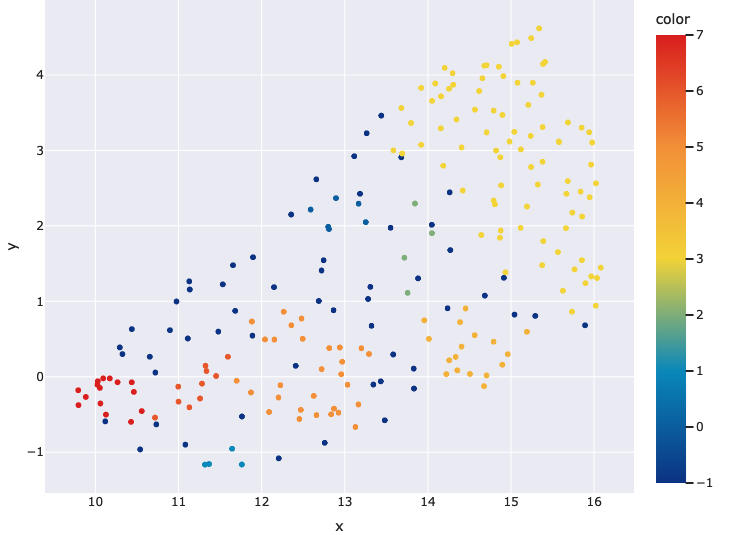
\includegraphics[width=\textwidth]{chapters/assets/c3lr_extra/c1.png}
     \end{subfigure}
     \hspace{1cm}
     \begin{subfigure}[b]{0.45\textwidth}
         \centering
         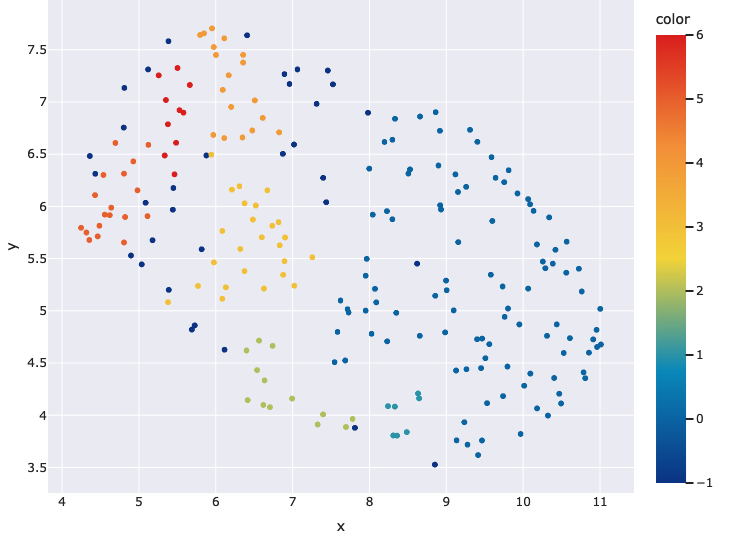
\includegraphics[width=\textwidth]{chapters/assets/c3lr_extra/c2.png}
     \end{subfigure}
     \label{fig:c3lr-hdbscan-results}
     \caption{Two plots showing the clusters generated by UMAP \parencite{mcinnes2018umap}. Notice the massive \textcolor{yellow}{yellow} and \textcolor{blue}{blue} clusters, it is unlikely all elements in them are truly similar. Unfortunately, due to the variable number of clusters generated by \texttt{HDBSCAN}, the legend is shown as a continuous colour scale to avoid repetition of colours. Cluster \textquote{$-1$} contains noisy points.}
\end{figure}


\subsection{Partial Compatibility with Gradient Based Learning}\label{ssec:c3lr-grad-based}

A major drawback of \ccclr{} is that the re-ranking and clustering steps are not compatible with gradient based learning. This means that any operations performed by these steps are not recorded in the computational graph tracked by PyTorch \parencite{pytorch2019}. A computational graph keeps track of all mathematical operations performed on a variable; during backpropagation this computational graph is used to calculate the gradients.
Due to this, information that is valuable to the model is lost between lines $8$ and $9$. The loss $\mathcal{L}_1$ is partially able to address this issue, however, it is far from ideal.

\chapter{\samptr{} Additional Materials}\label{sec:samptr-additional-mat}

This chapter covers the motivation for \samptr{}'s design choices as well as additional experiments with different types of graph neural networks.

Based on the discussion in \Cref{sec:ccclr-additional-mat}, there are three main issues with \ccclr{} that we have to address:
\begin{enumerate}
    \item There is no constraint on the amount of elements that can be placed within a cluster
    \item It is computationally heavy to compute new clusters in each training step 
    \item Partial compatibility with gradient-based learning hinders the network's learning ability (previous knowledge about re-ranking and clustering does not carry over).
\end{enumerate}

These problems with \ccclr{} formed the basis for certain design choices with respect to \samptr{}. In order to tackle problem (1), we do away with the clustering step and instead rely on self-attention based message passing to discover and refine features that belong to the same overarching class. In \ccclr{}, the clustering step was used to find similar data points in a batch. The same can be achieved by means of a self-attention message passing (SAMP) layer, because the SAMP layer can weigh the importance of each sample in its neighbourhood, it can also discover samples that are similar to each other.

For problem (2), we no longer need to use a heavy clustering and re-ranking steps. Both of these tasks can be handled by the self-attention message passing layer. Not only is it able to detect similar images in a batch (replaces clustering), it can also refine their features to bring them closer (replaces re-ranking).

For problem (3), as described in \cref{chap:gnn} graph neural networks are fully compatible with gradient based learning and optimisation. 


\section{Why SAMP?}\label{sec:why-samp}

\Cref{tab:gnn-types} shows the performance of three different types of GNNs. Before arriving on SAMP, we also tested the dynamic edge convolutions \parencite{wang2019dynamic} and LatentGNN \parencite{zhang2019latentgnn} layers.

\begin{table}[ht]
    \centering
    \begin{tabularx}{290pt}{Y Y Y}
    \toprule
        \textbf{Backbone} & \textbf{GNN Type} & \textbf{Accuracy} \\ 
        \midrule
        Conv4 & EdgeConv \citeyearpar{wang2019dynamic} & 57.76 $\pm$ 0.81 \\
        Conv4 & LatentGNN \citeyearpar{zhang2019latentgnn} & \underline{61.07} $\pm$ 0.66 \\
        Conv4 & SAMP  & \textbf{64.67} $\pm$ 2.65 \\
        \bottomrule
    \end{tabularx}
    \caption{Comparision between three types of GNN layers. Accuracy ($\%$ $\pm$ std.) values are for (\nwks{5}{5}) \miniImagenet{} classification tasks.}
    \label{tab:gnn-types}
\end{table}

We chose the EdgeConv layer because it has the ability to dynamically update the graph at every step. EdgeConv was originally developed to be used in processing 3D point cloud data, where it was meant to grasp the 3D structure of and relationships between the points of a scanned item.
We expected it to perform well with image feature vectors; however, due to the data changing too rapidly between training steps, it proved challenging for the EdgeConv layer to learn the similarities and relationships between images.

The next layer that we tested was the LatentGNN layer \parencite{zhang2019latentgnn}. It was developed for the express purpose of modelling non-local contextual relations between visual feature maps. The key idea is to introduce a latent space to reduce the complexity of the graph, which allows the use of a low-rank representation for the graph affinity matrix. \textcite{zhang2019latentgnn} insert this layer at intermediate points in a ResNet-$50$ and ResNet-$101$ \parencite{He2015}. The layer projects square feature maps to latent space as feature vectors and then applies message passing steps to refine the feature vectors and finally converts them back to square feature maps for further processing by convolution blocks.
Although this layer showed promising results, it requires a LatentGNN layer to be placed between convolutional layers, making a simple Conv$4$ unreasonably complex. However, the results were close enough to \ccclr{} and other competitors that it made natural sense to explore this direction further.

Ultimately, we arrive at a variant of the graph attention (GAT) layer \parencite{velic018graph} that we have coined as SAMP. SAMP has been formulated by \parencite{brody2021attentive,seidenschwarz2021learning}, among others. To the best of our knowledge, no one seems to have used it in the unsupervised few-shot learning context. It is simpler to use than LatentGNN and with minimal tuning the performance was within the margin of error of \ccclr{}.

\section{SAMP in Action}\label{sec:samp-in-action}

In \cref{fig:samp-training-emb-plots} the plot on the right shows image augmentations tightly grouped around the source image. From this we can infer that the SAMP layer is able to recognise similar images and refine their features so that they are closer in the representation space.
\begin{figure}[h]
     \centering
     \begin{subfigure}[b]{0.4\textwidth}
         \centering
         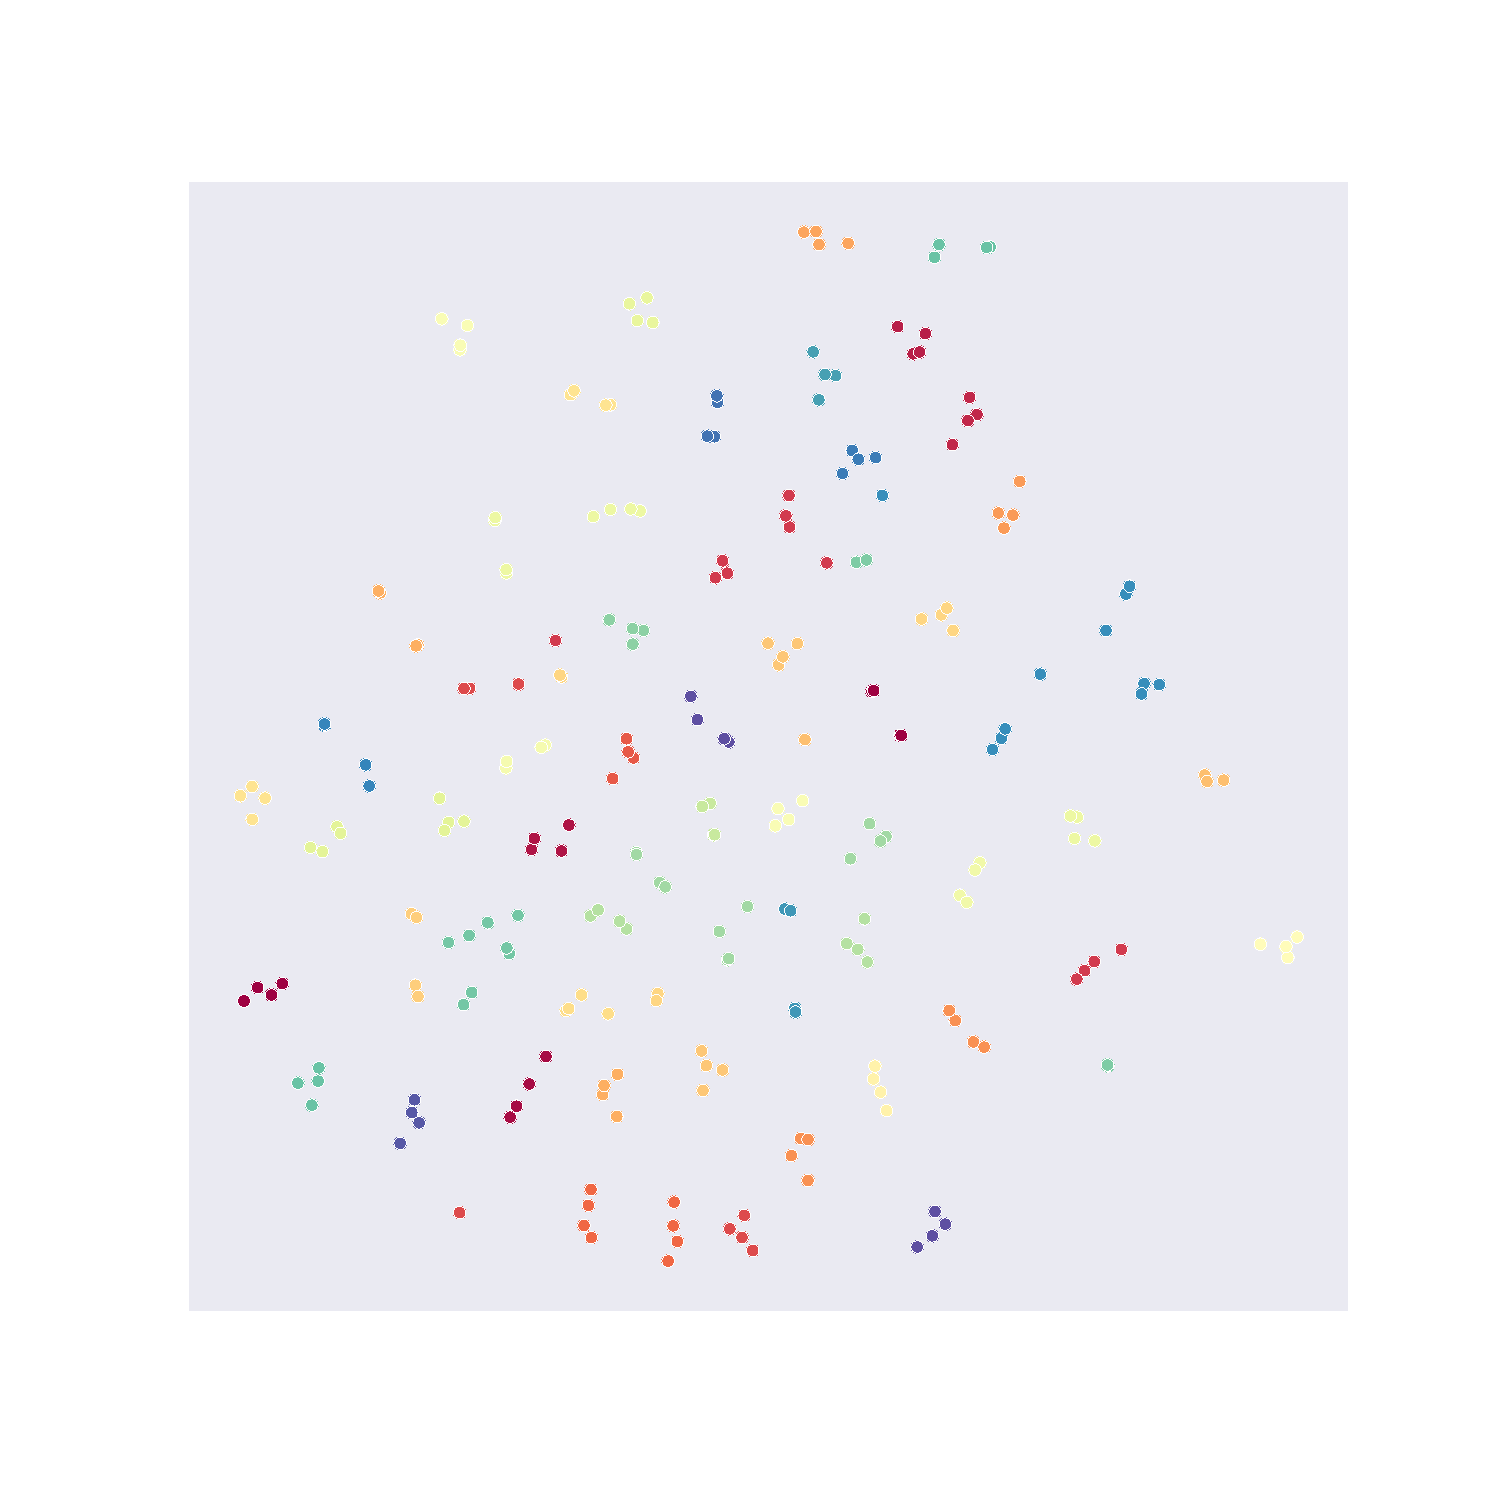
\includegraphics[width=\textwidth,trim=2.55cm 3cm 2.6cm 2.6cm, clip]{chapters/assets/samptr_extra/cnn_emb.pdf}
     \end{subfigure}
     \hspace{1cm}
     \begin{subfigure}[b]{0.4\textwidth}
         \centering
         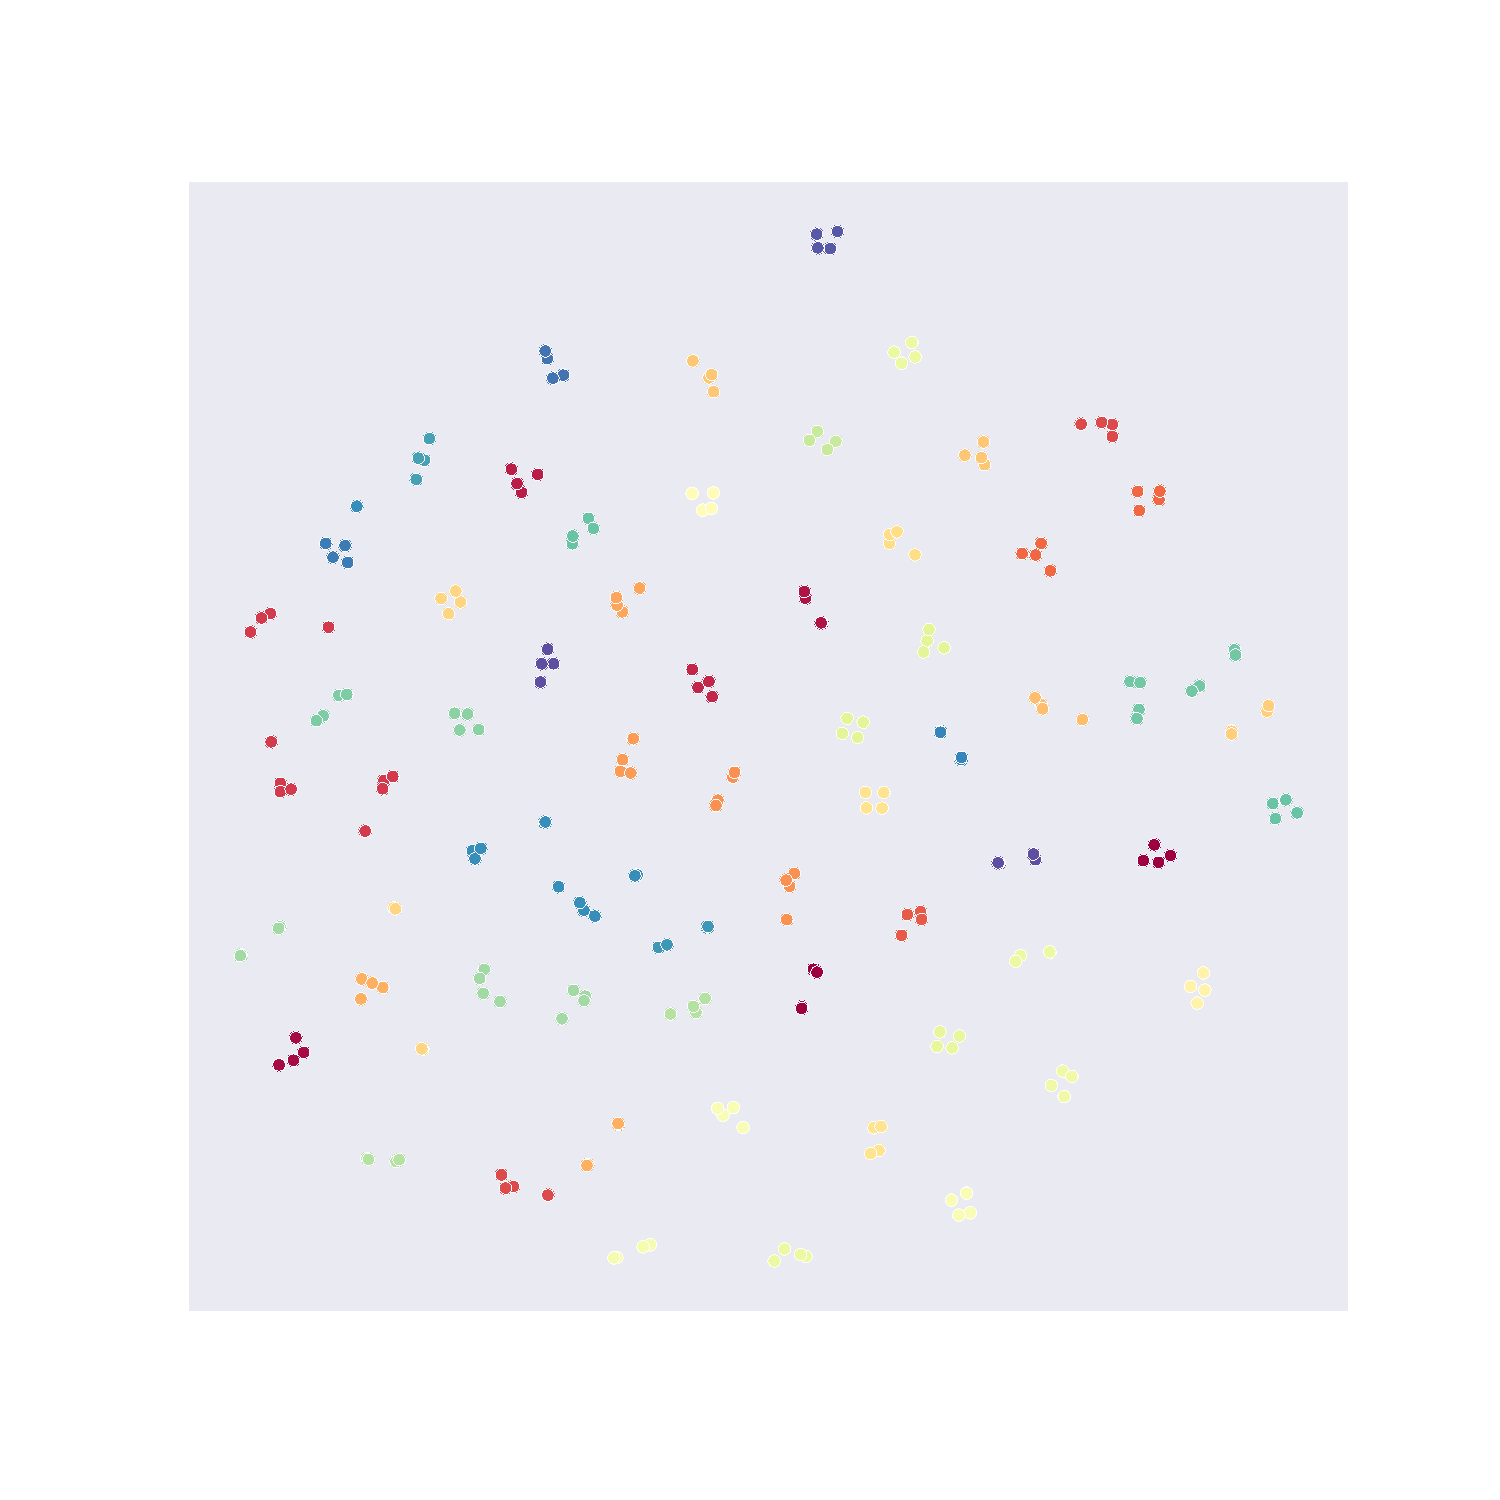
\includegraphics[width=\textwidth, trim=2.55cm 3cm 2.6cm 2.6cm, clip]{chapters/assets/samptr_extra/gnn_emb.pdf}
     \end{subfigure}
     \caption{ Each point is an image representation that has three neighbours which are its augmentations. The UMAP plot on the left shows features generated by the Conv$4$ backbone, the points are clearly more spread out. The flattened output of the Conv$4$ backbone are used as input to the SAMP layer. The UMAP plot on the right generated by using the SAMP layer outputs.
     }
     \label{fig:samp-training-emb-plots}
\end{figure}

Similar to \cref{fig:samp-training-emb-plots}, \cref{fig:samp-val-emb-plots} shows the embeddings of a support and query set in a (\nwks{2}{5}) task. We can see that the CNN features on the left aren't as separable, several \textcolor{orange}{orange} dots are in the are of the \textcolor{green}{green cluster}. However, when the CNN features are passed through a \texttt{SAMP} layer we can see that clusters form that are almost perfectly separable, indicating that the \texttt{SAMP} layer is working by looking beyond single instances and has learnt to refine features as required.

\begin{figure}[h]
     \centering
     \begin{subfigure}[b]{0.4\textwidth}
         \centering
         \includegraphics[width=\textwidth,trim=2.55cm 3cm 2.6cm 2.6cm, clip]{chapters/assets/samptr_extra/cnn_val_emb.pdf}
     \end{subfigure}
     \hspace{1cm}
     \begin{subfigure}[b]{0.4\textwidth}
         \centering
         \includegraphics[width=\textwidth, trim=2.55cm 3cm 2.6cm 2.6cm, clip]{chapters/assets/samptr_extra/gnn_val_emb.pdf}
     \end{subfigure}
     \caption{The figure on the left shows the CNN features of a support and query set from (\nwks{2}{5}) task drawn from the \miniImagenet{} validation set. The figure on the right shows the SAMP refined features where we can see two clearly separated clusters of points whereas on the right there are a few stray \textcolor{orange}{orange} points.}
     \label{fig:samp-val-emb-plots}
\end{figure}

\chapter{Conclusion and Future Work}\label{chap:future-work}

Inspired by the human mind's propensity to learn quickly and make new connections between known and unknown elements, this body of work introduces two novel ideas for self-supervised few-shot learning namely, \ccclr{} and \samptr{}.

%% Use letters for the chapter numbers of the appendices.
\appendix

%\input{appendix-a}

\printbibliography

\end{document}

